\documentclass[bachelor,lith,swedish]{liuthesis}
%% Settings go in settings.tex
\include{settings}
\usepackage{rotating}
\usepackage{color}
\usepackage{caption}
\usepackage{pgfplots}
\usepackage{pgf-pie}
\usepackage{float}

\department{Institutionen för datavetenskap}
\departmentenglish{Department of Computer Science}
\departmentshort{IDA}
% \externalsupervisor{Min företagshandledare}
\supervisor{Lena Buffoni}
\examiner{Kristian Sandahl}

\titleswedish{Visualisering av kontinuerlig integration}
% \subtitleswedish{}

\titleenglish{Visualization of continous integration}
% \subtitleenglish{}


\thesissubject{Datateknik}

\publicationyear{2017}
\currentyearthesisnumber{001}
\dateofpublication{2017-05-08}


%\author{\textttcc{\textbackslash author}}

% Two authors
\author{\parbox{\textwidth}{
    Joakim Argillander\\
    Victor Bodin \\
    Sebastian Callh\\
    Rebecca Lindblom \\
    Johan Nåtoft \\
    Johan Thornström \\
    Jonathan Wahlund\\
    Daniel Wassing}
}

\begin{document}

\chapterstyle{VZ43}
\renewcommand{\partname}{Del}
\pagestyle{plain}
\part{Gemensam del}
\chapter{Inledning}
\label{cha:inledning}
% the introduction should be divided into these two sections
Den här rapporten beskriver ett projektarbete i kursen TDDD96 Kandidatprojekt i mjukvaruutveckling. Arbetet utfördes under våren 2017 av en grupp bestående av åtta studenter från civilingenjörsprogrammen i datateknik och mjukvaruteknik vid Linköpings Universitet.
\\ \\
Rapporten innehåller dels beskrivning av uppgiften, hur den utfördes och vad resultatet blev. Efter detta diskuteras metoden och resultatet ur perspektivet av rapportens frågeställningar. Slutligen redovisas de  individuella utredningar som har utförts enskilt av alla gruppmedlemmar.

\section{Motivering}
\label{sec:motivering}
Kontinuerlig integration (KI) är en process för att integrera nya uppdateringar med befintlig version av en mjukvara. Varje ny uppdatering passerar genom ett flöde av tester, kompilering, granskningar med mera. Detta flöde genererar mycket information om hur väl den nya uppdateringen har presterat, men hur enkelt är det för intressenter i ett projekt att ta denna information till sig? En programmerare kanske främst vill veta hur väl hens uppdatering har klarat sig genom flödet, medan en person i högre chefsposition kan vara mer intresserad av att se helheten för utvecklingen. En chef kan till exempel vilja ha svar på följande frågor:
\begin{itemize}
\item Hur går utvecklingen? 
\item Hinner vi i tid till släpp av nästa version? 
\item Vilka moment tar mest tid?
\end{itemize}
\ \\
En chef utan teknisk spetskompetens kan dock ha svårt att ta till sig de stora mängden detaljerad information som kommer ur ett KI-flöde. Detta arbete gick ut på att utveckla en applikation som visualiserar denna data grafiskt och gör det lättare att tolka vad som sker i flödet.

%This is where the studied problem is described from a general
%point of view and put in a context which makes it clear that
%it is interesting and well worth studying. The aim is to make
%the reader interested in the work and create an urge to
%continue reading.

\section{Syfte}
\label{sec:purpose}
Med denna rapport avses att beskriva den arbetsmetodik som använts och hur ett system på ett lämpligt sätt kan visualisera data. Rapporten syftar också till att beskriva de tekniska resultat som erhållits i samband med genomförandet av detta projekt, samt redovisa de erfarenheter och förbättringsmöjligheter som framkommit under arbetet.

\section{Frågeställningar}
\label{sec:research-questions}

%This is where the research questions are described.
%Formulate these as explicit questions, terminated with a
%question mark. A report will usually contain several different
%research questions that are somehow thematically connected.
%There are usually 2-4 questions in total.

%Examples of common types of research questions (simplified
%and generalized):

\begin{enumerate}
\item Hur kan en webbapplikation för visualisering av kontinuerlig integration implementeras så att man skapar värde för kunden?
\item Vilka erfarenheter kan dokumenteras från programvaruprojekt "Visualisering av kontinuerlig
integration" som kan vara intressanta för framtida projekt?
\item Vilket stöd kan man få genom att skapa och följa upp en systemanatomi?
\item Hur kan man använda pappersprototyper för att underlätta kravinsamling? %beskriv vår process, så här kan man göra, BAM

%(Vad/vem/hur/vart är SEMAT Kernel BETA), kan nåtoft stava till SEMAT Kernel Alpha?

%\item How does technique X affect the possibility of achieving the
%  effect Y?

%\item How can a system (or a solution) for X be realized so
%  that the effect Y is achieved?

%\item What are the alternatives to
%  achieving X, and which alternative gives the best effect considering
%  Y and Z? (This research question is normally broken down in to 2
%  separate questions.)

\end{enumerate}


%Observe that a very specific research question almost always
%leads to a better thesis report than a general research question
%(it is simply much more difficult to make something good
%from a general research question.)

%The best way to achieve a really good and specific research
%question is to conduct a thorough literature review and get
%familiarized with related research and practice. This leads to
%ideas and terminology which allows one to express oneself
%with precision and also have something valuable to say in the
%discussion chapter. And once a detailed research question
%has been specified, it is much easier to establish a suitable
%method and thus carry out the actual thesis work much faster
%than when starting with a fairly general research question. In
%the end, it usually pays off to spend some extra time in the
%beginning working on the literature review. The thesis
%supervisor can be of assistance in deciding when the research
%question is sufficiently specific and well-grounded in related
%research.

\section{Avgränsningar}
\label{sec:delimitations}
%Rapporten kommer att behandla projektets utvecklingsfaser och slutprodukt
%vilket gör att specifika saker, som t.ex. implementations- och systemdetaljer,
%inte kommer nämnas.
%Målgruppen för rapporten är studenter, handledare och examinatorer vid kursen
%TDDD96: Kandidatprojekt i programvaruutveckling vid Linköpings universitet.

De avgränsningar som appliceras på applikationen täcker en rad områden. Applikationen är ett verktyg för visualisering och utför därför ingen databehandling. Den är anpassad för större skärmar och därmed inte optimal på mindre skärmar och handhållna enheter. Den är utvecklad med stöd för endast engelska.
\begin{table}[h!]
  \centering
  \caption{En tabell över utvecklingsplattformar.}
  \def\arraystretch{1.5}
  \begin{adjustbox}{max width=\textwidth}
    \begin{tabularx}{\textwidth}{ | l | X | }
      \hline
      \textbf{Operativsystem} & \textbf{Webbläsare} \\
      \hline
      Ubuntu 16.04 & Firefox 51.0.1 \\
      \hline
      macOS Sierra 10.12.3 & Chrome 55.0.2883.95 \\
      \hline
      Windows 8.1, 10 & Chrome 55.0.2883.95 \\
      \hline
    \end{tabularx}
  \end{adjustbox}
  \label{tab:utvecklingsplattformar}
\end{table}
\ \\
Utveckling och testning har skett på ett begränsat antal plattformar som kan ses i tabell \ref{tab:utvecklingsplattformar} vilket har lett till att applikationen inte är garanterad att fungera på andra plattformar. Utvecklingen av applikationen har utförts med hjälp av ramverket Meteor. Valet att utveckling skulle ske med hjälp av Meteor beslutades efter ett möte med kund, vilket gjorde att andra tänkbara ramverk för applikationer valdes bort.

%\nocite{scigen}
%We have included Paper \ref{art:scigen}


\chapter{Bakgrund}
\label{cha:background}
Även om KI-system implementeras för att hantera komplexitet, kan även de
bli komplexa och svåröverskådliga. Konsortiet Software Center arbetar tillsammans med
bland annat Linköpings Universitet för att studera storskaliga mjukvarumiljöer
för kontinuerlig integration och det var de som lade grunden för det här projektet.
\\ \\ 
Kunden för detta projekt var Kristian Sandahl och Ola Leifler ifrån Institutionen
för datateknik (IDA) på Linköpings Universitet som på Software Centers vägnar ville ha
en webbapplikation för att visualisera KI-system. Målet var att ge ett beslutsstöd
för intressenter utan teknisk kompetens genom att på ett lättöverskådligt
sätt kunna identifiera flaskhalsar och eventuella problem i KI-system.
\\ \\
Projektet utfördes som en del av kursen TDDD96 Kandidatprojekt i programvaruutveckling
av åtta studenter från civilingenjörsprogram i datateknik och mjukvaruteknik.
Tillsammans med projektdirektivet tillhandahölls även en tidigare utvecklad
prototyp av systemet.

%I samarbete med konsortiet Software center, med 10 företag och 5
%universitet, arbetar vi med att studera storskaliga miljöer för kontinuerlig integration (CI).
%Idag har dessa miljöer vuxit i komplexitet samtidigt som möjligheterna för att gå ännu
%längre – kontinuerlig leverans – blir lockande för företagen.

%%% lorem.tex --- 
%% 
%% Filename: lorem.tex
%% Description: 
%% Author: Ola Leifler
%% Maintainer: 
%% Created: Wed Nov 10 09:59:23 2010 (CET)
%% Version: $Id$
%% Version: 
%% Last-Updated: Tue Oct  4 11:58:17 2016 (+0200)
%%           By: Ola Leifler
%%     Update #: 7
%% URL: 
%% Keywords: 
%% Compatibility: 
%% 
%%%%%%%%%%%%%%%%%%%%%%%%%%%%%%%%%%%%%%%%%%%%%%%%%%%%%%%%%%%%%%%%%%%%%%
%% 
%%% Commentary: 
%% 
%% 
%% 
%%%%%%%%%%%%%%%%%%%%%%%%%%%%%%%%%%%%%%%%%%%%%%%%%%%%%%%%%%%%%%%%%%%%%%
%% 
%%% Change log:
%% 
%% 
%% RCS $Log$
%%%%%%%%%%%%%%%%%%%%%%%%%%%%%%%%%%%%%%%%%%%%%%%%%%%%%%%%%%%%%%%%%%%%%%
%% 
%%% Code:

\chapter{Teori}
\label{cha:theory}
De fakta som presenteras i denna rapport är hämtade från \textit{Documentation in System Development: A significant Criterion for Project Success} \cite{docsystemdev}, \textit{Collaborating with ShareLaTeX and git} \cite{website:sharelatex_with_git} samt \textit{How SciGit and other collaborative editing/version control services are different} \cite{website:scigit_blog}. \\
Fakta presenteras även från intervjuer som har skett under projektets gång.
\\ \\
Nedan presenteras ett flertal av de olika verktyg som tillfrågade personer från olika grupper har använt sig av. Dessa verktyg är de som kommer att behandlas i denna rapport.

\section{LaTeX}
\LaTeX (Lamport TeX) är ett s.k. \textit{märkspråk}\footnote{Märkspråk är mer känt som Markup Language på engelska} för att producera dokument, precis som \textit{HTML}\footnote{HTML är en förkortning av HyperText Markup Language} är ett märkspråk för webbprogrammering. \\
LaTeX skapades av \textbf{Leslie Lamport}. Den senaste versionen heter LaTeX2e och släpptes 1994, med mindre uppgraderingar som släpps ungefär varje halvår.
\\ \\
LaTeX bygger på typsättningssystemet \textit{TeX} som utvecklades av \textbf{Donald Knuth} under 1970 och 1980-talet \cite{the_tex_book}. Språkdefinitionen blev fastställd under 1985.
\\ \\
LaTeX används i dag främst i vetenskapliga kretsar, framför allt inom områdena matematik, fysik och datavetenskap. Det omfattar dokumentstilar för artiklar, böcker, brev, presentationer med mera samt stöd för referenser och automatisk numrering av avsnitt och ekvationer. LaTeX är förmodligen det vanligaste sättet att utnyttja grundprogrammet TeX då det finns väldigt mycket funktionalitet färdig från början, utan att man behöver importera och/eller använda annan mjukvara. LaTeX kan generera en mängd dokumentformat, den vanligaste är PDF.

\section{Git}
\label{sec:wassing-git}
\textit{Git} \cite{website:git} är ett versionshanteringsprogram \cite{website:git_version_control} som skapades 2005 av \textbf{Linus Torvalds} för att hantera källkod till Linuxkärnan\footnote{Linux är ett operativsystem som Linus Torvalds publicerade 1991}. Git kan jämföras med \textit{CVS} eller \textit{Subversion} som också är versionshanteringssystem. Till skillnad från de andra två är däremot Git de-centraliserat \cite{website:centralized_version_control}, vilket betyder att det inte finns ett mäster-arkiv som alltid har den senaste versionen av ändringar. CVS och Subversion tas ej upp här då ingen tillfrågad grupp har använt sig av de systemen.
\\ \\
Git är främst tänkt för filer med oformatterad text, men har på senare tid fått utökad support för binära filer såsom Microsoft Word dokument. Detta kräver dock plugins som ofta bara konverterar binära filer till oformatterad text. \cite{website:using_git_with_word} Användandet av olika plugins gör ofta att Git inte är ett alternativ när man jobbar med binära filer. Mer om det i avsnitt \ref{cha:wassing-discussion}.

\section{Google Drive}
\textit{Google Drive} \cite{website:googledrive}, även tidigare känt som \textit{Google Docs}, är en molntjänst som tillhandahålles konstnadsfritt av Google. Google Drive ses ofta som Googles motsvarighet till Microsofts Officepaket (som inkluderar bland annat Word). Genom Google Drives molntjänst så kan användare redigera i samma dokument samtidigt. Dessutom kan även andra filer laddas upp och delas. Google Drive kräver en internetanslutning för att användare ska kunna komma åt dokumenten, men är i övrigt helt oberoende av mjukvara. Det finns möjlighet att exportera dokument som skrivs i Google Drive till andra format, bland annat PDF.

\section{ShareLaTeX}
\textit{ShareLaTeX} \cite{website:sharelatex} kan liknas vid Google Drive, fast med att skriva dokument i LaTeX som huvudfunktion. ShareLaTeX  är likt Google Drive plattformsoberoende och exekverar direkt i webbläsaren. Det finns en enorm support för olika LaTeX och TeX bibliotek och plugins, vilka alla kan kallas på direkt i dokumenten när man skriver online utan att vidare arbete behöver utföras. ShareLaTeX har även ett begränsat stöd för att arbeta med Git sedan hösten 2015.
\\ \\
Likt LaTeX så används ShareLaTeX primärt för att skapa PDF-filer av hög kvalitet.

\section{Microsoft Office}
\textit{Microsoft Office} är en paketlösning från Microsoft som innehåller de populära prorammen Word, Excel och Powerpoint med flera. Officepaketet är en köpvara, men studenter på LIU kan få det gratis genom Lisam \cite{website:liu_office_package}. Word tillåter skapandet av högteknologiska dokument genom ett stort antal funktioner. Word har däremot ingen inbyggd delningsfunktion, vilket gör att inte mer än en person åt gången kan jobba med ett dokument.
\\ \\
I senare versioner av Office så finns det även möjligheten att exportera till andra filformat än de typiska som mjukvara i Office använder sig av (.doc, .xls och .ppt). Microsoft Office är fortfarande industriell standard. Det erbjuds fortfarande utbildning i Microsoft Office i elementära skolår och gymnasiet än i dag.

%The main purpose of this chapter is to make it obvious for
%the reader that the report authors have made an effort to read
%up on related research and other information of relevance for
%the research questions. It is a question of trust. Can I as a
%reader rely on what the authors are saying? If it is obvious
%that the authors know the topic area well and clearly present
%their lessons learned, it raises the perceived quality of the
%entire report.

%After having read the theory chapter it shall be obvious for
%the reader that the research questions are both well
%formulated and relevant.

%The chapter must contain theory of use for the intended
%study, both in terms of technique and method. If a final thesis
%project is about the development of a new search engine for
%a certain application domain, the theory must bring up related
%work on search algorithms and related techniques, but also
%methods for evaluating search engines, including
%performance measures such as precision, accuracy and
%recall.

%The chapter shall be structured thematically, not per author.
%A good approach to making a review of scientific literature
%is to use \emph{Google Scholar} (which also has the useful function
%\emph{Cite}). By iterating between searching for articles and reading
%abstracts to find new terms to guide further searches, it is
%fairly straight forward to locate good and relevant
%information, such as \cite{test}.

%Having found a relevant article one can use the function for
%viewing other articles that have cited this particular article,
%and also go through the article’s own reference list. Among
%these articles on can often find other interesting articles and
%thus proceed further.

%It can also be a good idea to consider which sources seem
%most relevant for the problem area at hand. Are there any
%special conference or journal that often occurs one can search
%in more detail in lists of published articles from these venues
%in particular. One can also search for the web sites of
%important authors and investigate what they have published
%in general.

%This chapter is called either \emph{Theory, Related Work}, or
%\emph{Related Research}. Check with your supervisor.


%%%%%%%%%%%%%%%%%%%%%%%%%%%%%%%%%%%%%%%%%%%%%%%%%%%%%%%%%%%%%%%%%%%%%%
%%% lorem.tex ends here

%%% Local Variables: 
%%% mode: latex
%%% TeX-master: "demothesis"
%%% End: 

%%%%%%%%% lorem.tex --- 
%% 
%% Filename: lorem.tex
%% Description: 
%% Author: Ola Leifler
%% Maintainer: 
%% Created: Wed Nov 10 09:59:23 2010 (CET)
%% Version: $Id$
%% Version: 
%% Last-Updated: Wed Nov 10 09:59:47 2010 (CET)
%%           By: Ola Leifler
%%     Update #: 2
%% URL: 
%% Keywords: 
%% Compatibility: 
%% 
%%%%%%%%%%%%%%%%%%%%%%%%%%%%%%%%%%%%%%%%%%%%%%%%%%%%%%%%%%%%%%%%%%%%%%
%% 
%%% Commentary: 
%% 
%% 
%% 
%%%%%%%%%%%%%%%%%%%%%%%%%%%%%%%%%%%%%%%%%%%%%%%%%%%%%%%%%%%%%%%%%%%%%%
%% 
%%% Change log:
%% 
%% 
%% RCS $Log$
%%%%%%%%%%%%%%%%%%%%%%%%%%%%%%%%%%%%%%%%%%%%%%%%%%%%%%%%%%%%%%%%%%%%%%
%% 
%%% Code:

\chapter{Metod}
\label{cha:method}

In this chapter, the method is described in a way which shows how the
work was actually carried out. The description must be precise and
well thought through. Consider the scientific term
replicability. Replicability means that someone reading a scientific
report should be able to follow the method description and then carry
out the same study and check whether the results obtained are
similar. Achieving replicability is not always relevant, but precision
and clarity is.

Sometimes the work is separated into different parts, e.g.  pre-study,
implementation and evaluation. In such cases it is recommended that
the method chapter is structured accordingly with suitable named
sub-headings.

\section{Förstudie}
\label{sec:pre-study}

Retrospective är ett välanvänt verktyg bland de team som använder sig av Scrum och många har t.o.m. forskat
kring metoderna med agilutveckling. Därför har den här studien använt sig mycket av publicerade artiklar om agil arbetsmetodik
samt ett par böcker om hur man främst jobbar tillsammans i grupp. Samtliga artiklar och böcker går att finna bland referenserna.
Då den här rapporten är resultatet av dels en litterär studie och en praktisk studie så behövdes ett praktiskt sammanhang att undersöka.
Rapporten är en del av kursen TDDD96: 'Kandidatprojekt i programvaruutveckling' så sammanhanget blev det projekt som grupp 2 fick att genomföra.
Som nämnt i Introduktionen så Retrospective en del av Scrum och något som ska göras i slutet av varje iteration.
Då arbetsgruppen aldrig använt sig av Scrum som agil arbetsmetod så beslutades det att samtliga delar av Scrum skulle implementeras och därmed
även Retrospective-utvärderingar.

\section{Implementation}
\label{sec:implementation}

Längden av varje iteration under gruppens arbete sattes till 2 veckor långa och gav därmed utvärderingstillfälle med 2 veckors mellanrum.
Det planerades in ett 2 timmar långt tillfälle då samtliga av gruppens medlemmar kunde närvara vid slutet av iterationen och sedan genomfördes utvärderingen med ledning av team-ledaren. 

\subsubsection{Retrospective}
Den här delen ska förklara lite mer utförligt vad Retrospective är och vilka delar som ingår i en utvärdering av den typen.\\ \\
\textbf{Datainsamling}\\
Den första delen är datainsamlingen. Datainsamlingen i sig är uppdelad i 4 delar där den första delen är 'Teamutvärdering'. 
Här så får alla gruppmedlemmarna ett papper med ett flertal uttryck som de ska rangordna från 1-5 beroende på hur mycket de håller med uttrycket \cite{Team-utvärderings-pappret}. 
Den andra delen av datainsamlingen är 'Nöjdhet', där gruppens medlemmar ska svara på frågan 'Hur nöjda är vi med vårt arbete?'. Även här ska man svara enligt en 5-gradig skala.
\begin{itemize}
\item 5 = Jag tycker att vi är det bästa teamet på planeten. Vi jobbar bra ihop!
\item 4	= Jag är glad att jag är en del av teamet och nöjd med hur vårt team arbetar tillsammans
\item 3	= Jag är ganska nöjd. Vi jobbar bra tillsammans för det mesta
\item 2	= Jag har några stunder av tillfredsställelse, men inte tillräckligt
\item 1	= Jag är olycklig och missnöjd med vår nivå av lagarbete
\end{itemize}

Den tredje delen av datainsamlingen är 'Sammanställning', där man först identifierar de uttrycken eller områden som fått 1 eller 2 poäng av vardera gruppmedlem. Sedan sammanställer man gruppmedlemmarnas svar och fokuserar då främst på de som angett 1 eller 2 poäng.
Den sista delen av datainsamlingen är 'Bra \& Bättre', där man jobbar med frågorna.
\begin{itemize}
\item Vad är vi bra på?
\item Vad kan vi bli bättre på?
\end{itemize}
Man gör detta genom att varje gruppmedlem får en bunt post-it lappar. På lapparna så skriver varje medlem ner något som gruppen då är bra på eller kan bli bättre på med en åsikt per lapp. Efter att alla fått ihop några lappar var så går man sedan igenom lapparna genom att varje gruppmedlem läser upp en lapp i taget och sedan går man laget runt tills det inte längre finns några lappar kvar att läsa upp.

Nästa del av utvärderingen är 'Insikter'. Den här delen fungerar ungefär precis som 'Bra \& Bättre' från datainsamlingen, alltså på det sättet att varje gruppmedlem får en bunt post-it lappar att skriva på för att man sedan går igenom dessa lappar laget runt. I det här fallet ska man dock skriva ner vilka förbättringsförslag man har till de eventuella problem som identifierades under 'Bra \& Bättre'.

Efter att alla fått presentera sina förbättringsförslag så sammanställs dessa under nästa del som är 'Åtgärder'. Här bestämmer gruppen gemensamt vilka förbättringsförslag gruppen ska anamma och jobba med under nästa iteration av arbetet.

Den sista delen av utvärderingen är en kort summering och återkoppling på det som gåtts igenom. Här lyfts de saker som gruppen valde att fokusera på fram så att det blir tydligt vad som ska fokuseras på som förbättring under nästa iteration.
Man avslutar med att identifiera 3 saker som gruppen gjorde bra under retrospektivet.


%%%%%%%%%%%%%%%%%%%%%%%%%%%%%%%%%%%%%%%%%%%%%%%%%%%%%%%%%%%%%%%%%%%%%%
%%% lorem.tex ends here

%%% Local Variables: 
%%% mode: latex
%%% TeX-master: "demothesis"
%%% End: 

\chapter{Resultat}
\label{cha:results}
I detta kapitel presenteras resultaten som projektet har genererat. Resultaten är bland annat den faktiska webbapplikation som producerats samt de erfarenheter som gruppen dragit på sig under projektets gång. Det ges även en kort översikt av de individuella fördjupningar som gruppens medlemmar genomfört.
\section{Testning}
Under projektets gång utvecklade gruppen en testmetodik för att kunna verifiera att applikationen möter de krav som etablerats i kravspecifikationen. Vid projektets start skapades en övergripande testplan som beskrev en förlaga till den testmetodik som utvecklades under projektet. Då gruppen såg framtagandet av testningsprocesser som ett kontinuerligt arbete så kunde dessa utvecklas inkrementellt utifrån gruppens erfarenheter, färdigheter och förväntningar från tidigare iterationer. Vartefter projektet fortlöpte tillkom testuppgifter, olika testverktyg utvärderades och metoder för att frambringa spårbarhet i testningsprocessen togs fram. Detta resulterade i ett ramverk för testning anpassat för mindre utvecklingsgrupper arbetandes efter agila principer.

\section{Prototyper}
\label{sec:result-prototypes}
De slutgiltiga övergripande prototyperna skapades i pappersform, och gjordes delvis interaktiva i verktyget InVision. 

\begin{figure}[H]
    \centering
    \includegraphics[scale=0.65]{prototype-aggregation}
    \caption{Prototyp för den aggregerade vyn och händelse vid placering av muspekaren på en nod.}
    \label{fig:prototype-aggregation}
\end{figure}
\ \\
Skiss för den aggregerade vyn syns i figur \ref{fig:prototype-aggregation}. 
I skissen finns en yta för en aggregerad graf, där grafens noder representerar en händelsetyp i KI-flödet. 
De flerfärgade noderna illustrerar grad av godkända körningar för den händelsetypen. Den översta noden i mitten visar en förstorad nod då muspekaren placeras på noden. 
Rutan innehåller mer detaljerad information om händelserna i noden. Vid klick på rutan navigerar applikationen till nästa vy. 
Grafens ruta inkluderar även en navigeringspanel med zoom-reglage, samt en ikon för hjälp. 
Under grafens ruta finns en tidslinje för att filtrera ut händelser från ett visst tidsspann. 

\begin{figure}[H]
    \centering
    \includegraphics[scale=0.5]{niva2}
    \caption{Prototyp för diagramläget samt tabelläget för den detaljerade vyn.}
    \label{fig:prototype-details}
\end{figure}
\ \\
I figur \ref{fig:prototype-details} visas prototypen för den detaljerade vyn, som innehåller detaljer om en specifik händelsetyp. 
Där kan användaren välja att visa ett tabelläge eller ett diagramläge. Tabelläget visar en rad för varje händelse i noden, och den kan sorteras baserat på alla kolumner. 
Vid växling till diagramläget visas olika data för noden över tid. 
På den horisontella axeln visas tid, och på den vertikala axeln kan användaren välja någon data genom att bläddra i rullistan. 

\begin{figure}[H]
    \centering
    \includegraphics[scale=0.5]{niva3}
    \caption{Prototyp för ett händelseflöde.}
    \label{fig:prototype-eventchain}
\end{figure}
\ \\
Den tredje vyn är en graf som visar ett enskilt händelseflöde, se figur \ref{fig:prototype-eventchain}. 
I denna graf är varje nod en specifik händelse. 
I den förstorade rutan vid placering av muspekare på en nod finns en länk för att öppna händelsen i programmet som genererade den.

\section{Systembeskrivning}
Denna del beskriver det system som gruppen har tagit fram och ger en överblick på hur systemet fungerar.
\label{sec:results-systemoverview}
\begin{figure}[h]
    \centering
    \includegraphics[scale=0.5]{Systemskiss}
    \caption{Översikt av systemet.}
    \label{fig:architectural_overview}
\end{figure}
\\
En översikt av systemet ges i figur.\ref{fig:architectural_overview} Systemet består av en klient och en server. Både klienten och servern har utvecklats i ramverket Meteor för JavaScript. Servern sköter all hämtning av data från databasen och levererar den till klienten. Klienten används för all visualisering av Eiffeldata. Den hämtar Eiffelhändelser från servern och visualiserar dom i webbläsaren. De Eiffelhändelserna sparas ner i en lokal databas med namnet Mini Mongo. Klienten är en \textit{Single-page application} vilket betyder att sidan bara behöver laddas en gång när den startas, så att de individuella delarna på sidan uppdateras dynamiskt utan att behöva ladda om sidan som leder till en bättre användarupplevelse.
\\ \\
Applikationens filstruktur följer Meteors rekommenderade standard.\cite{website:meteorstructure} Den följer även Meteors rekommenderade kodstil för hur kod till en applikation implementeras.\cite{website:meteorcodestyle} En tydlig struktur för projektet ger applikationen en enhetlig standard vilket ökar läsbarheten för utvecklaren.

\subsection{Systemanatomi}
\label{subsec:results_anatomy}
En systemanatomin togs fram baserat på de funktionella kraven från kravspecifikationen och användningsfall.
\begin{figure}[H]
    \centering
    \includegraphics[scale=0.35]{Systemanatomi}
    \caption{Systemets anatomi.}
    \label{fig:systemanatomi}
\end{figure}
\ \\I figur \ref{fig:systemanatomi} visas systemanatomin för applikationen. Där de primära användarfunktioner för systemanatomin är högst upp i figuren.

\subsection{Moduler}
\label{subsec:results-modules}
\begin{figure}[h]
    \centering
    \includegraphics[scale=0.5]{moduler}
    \caption{Översikt av klientens moduler.}
    \label{fig:module_overview}
\end{figure}
\ \\
I figur \ref{fig:module_overview} ges en översikt över de moduler som används i applikationen. Applikationens klient är uppdelad i fyra moduler som hanterar de olika typer av funktionalitet som används. I följande lista finns de modulerna och deras uppgift.
\begin{itemize}
  \item Aggregation.js - Innehåller de funktionsanrop som behövs i de aggregerade graferna.
  \item Eventchain.js - Innehåller de funktionsanrop som behövs när en nod från den aggregerade grafen visas i tabelläge eller diagramläge.
  \item Details.js - Innehåller funktionsanrop för händelseflöde och har precis som aggregation.js i uppgift att rendera grafer.
  \item Graph.js - Är modulen där all rendering av grafer för aggregering och händelseflöden sker. Graph.js använder sig av två externa bibliotek: Cytoscape.js för rendering av graferna och Dagre.js för dess layout.
\end{itemize}

\section{Användargränssnitt}
\label{sec:results-gui}
%\textbf{TODO:}
%\begin{itemize}
%\item Ändra färgers representation om dessa ändras i GUI:t
%\item Hjälprutans innehåll
%\end{itemize}
Systemet visar data i tre olika vyer. De tre vyerna är placerade under varandra och vid start presenteras den översta vyn. För att navigera mellan de olika vyerna finns dels funktionalitet i varje vy som beskrivs i följande avsnitt, men också en allmän navigationspanel på höger sida. Vid klick på knapparna för vyerna kommer det visade området att förflyttas till den valda vyn. Hela panelen följer med och syns alltid på skärmen oavsett vilken vy som visas.

\begin{figure}[H]
  \centering
  \includegraphics[scale=0.33]{gui_aggregation}
  \caption{Aggregeringsvyn med navigationspanelen till höger.}
  \label{fig:gui_aggregation}
\end{figure}
\ \\
Panelen innehåller även informationsknapp för att öppna en hjälpruta, samt en indikator för uppkoppling mot servern, vilket visas till höger i figur \ref{fig:gui_aggregation}.  

\begin{figure}[H]
  \centering
  \includegraphics[scale=0.33]{gui_helpmodal}
  \caption{Hjälprutan har öppnats ovanpå den aggregerade vyn.}
  \label{fig:gui_helpmodal}
\end{figure}
\ \\
Hjälprutan som visas i figur \ref{fig:gui_helpmodal} innehåller information om hur applikationen används.

\begin{figure}[H]
  \centering
  \includegraphics[scale=0.6]{gui_connection}
  \caption{Informationsruta som dyker upp om klienten tappar kontakten med servern.}
  \label{fig:gui_connection}
\end{figure}
\ \\
Indikatorn för uppkoppling mot server är grön då klienten är ansluten till servern. Vid tappad anslutning dyker en informationsruta upp som informerar om att anslutningen är bruten samt eventuell anledning, se figur \ref{fig:gui_connection}. Indikatorn blir då röd.

\begin{figure}[H]
  \centering
  \includegraphics[scale=0.8]{gui_loading}
  \caption{Symbol för att indikera att klienten väntar på svar från servern.}
  \label{fig:gui_loading}
\end{figure}
\ \\
I figur \ref{fig:gui_loading} syns symbolen som roterar över skärmen då klienten väntar på svar på ett anrop till servern.

\subsection{Aggregering}
Aggregeringen representeras av en riktad acyklisk graf, och visar Eiffel-händelser som skett i KI-flödet, se figur \ref{fig:gui_aggregation}. Varje nod i grafen är en typ av händelse, och innehåller i sin tur varje enskild händelse av den typen. Bågarna pekar på den föregående händelsen i flödet. Noderna har olika former baserat på dess händelsetyp.
\\ \\
Vissa noder är händelser som har en status, exempelvis av implementationen definierade aktiviteter, eller körningar av testfall och testsviter. Dessa noder har olika färgfyllningar beroende på dess status. En nod för testfall som har 70\% klarade fall kommer att visas som en ruta med 7/10 grönt och 3/10 rött. 

\begin{figure}[H]
  \centering
  \includegraphics[scale=0.8]{gui_aggregation_tooltip}
  \caption{En informationsruta öppnas vid klick på en nod.}
  \label{fig:gui_aggregation_tooltip}
\end{figure}
\ \\
Vid klick på en nod dyker en informationsruta upp, som är kopplad till noden, se figur \ref{fig:gui_aggregation_tooltip}. Rutan innehåller mer detaljerad information, som till exempel antal händelser i noden och mer detaljer om händelsernas eventuella status. Informationsrutan innehåller även en knapp för att öppna den detaljerade vyn för den valda händelsetypen.
\\ \\
Under grafen visas en tidslinje, där det är möjligt att filtrera vilka händelser som visas, se figur \ref{fig:gui_aggregation}. Användaren kan zooma in i tidslinjen genom att scrolla, och då kommer varje steg i tidslinjen representeras av en mindre enhet tid. Minsta möjliga enhet är 10 minuter. 
Det finns två flyttbara markörer, en för starttid och en för sluttid. Vid förflyttning av dessa skickas ett anrop till servern som returnerar en ny filtrering av händelser. Markörerna kan maximalt flyttas till de tidpunkter då den första respektive sista händelsen i databasen ägde rum. Användaren kan även välja start och sluttid genom att fylla i boxarna för start och sluttid under tidslinjen.

\subsection{Detaljerad vy över en händelsetyp}
Den detaljerade vyn visar all data för varje händelse. Denna vy har två olika lägen, ett tabelläge och ett diagramläge. 
\begin{figure}[H]
  \centering
  \includegraphics[scale=0.33]{gui_details}
  \caption{Den detaljerade vyns tabelläge.}
  \label{fig:gui_details}
\end{figure}
\ \\
I tabelläget som öppnas som standard visas varje enskild händelse som en rad i tabellen, se figur \ref{fig:gui_details}. Tabellen har kolumner som speglar varje händelsetyps datainnehåll, till exempel tidsstämpel eller teststatus. Det är möjligt att sortera tabellen i stigande eller fallande ordning med avseende på valfri data genom att klicka på kolumnens rubrik. Då dyker en symbol upp som visar i vilken ordning det är sorterat. Varje rad innehåller en knapp för att navigera till händelseflödet för den aktuella händelsen.
\begin{figure}[H]
  \centering
  \includegraphics[scale=0.33]{gui_details_plot}
  \caption{Den detaljerade vyns diagramläge.}
  \label{fig:gui_details_plot}
\end{figure}
\ \\
Reglaget ovanför tabellen används för att navigera till diagramläget, se figur \ref{fig:gui_details_plot}. I diagramläget visas en funktionskurva som visar förändringar över tid hos en viss data i händelsetypen.

\subsection{Händelseflöden}
Ett händelseflöde representeras av en liknande graf som i aggregeringen. Skillnaden är att denna vy inte är aggregerad, alltså är varje nod en enskild händelse. 
\begin{figure}[H]
  \centering
  \includegraphics[scale=0.33]{gui_eventchain_tooltip}
  \caption{Ett händelseflöde, med en öppnad informationsruta.}
  \label{fig:gui_eventchain_tooltip}
\end{figure}
\ \\
Varje händelseflöde inleds med en kodändring, men då alla kodändringar är länkade till varandra i ett cykliskt beroende kapas länkarna från dessa och skapar \textit{sekvenser} av de resterande händelserna fram till en förändring av pålitlighetsgrad.
En händelse tillhör exakt en sekvens, men kan ha kopplingar till händelser i separata sekvenser. Detta kopplingar är oföljda länkar och representeras i grafen med streckade bågar. Den närmast närliggande sekvensen ritas ut, men dess egna oföljda länkar visas inte. På så sätt innehåller varje händelseflöde en eller flera sekvenser, med en kodändring som initiering.
\\ \\
Denna graf visar händelsetyp för varje nod samt eventuell status precis som i den aggregerade grafen, men då noderna endast representerar en händelse är de enfärgade. Den händelse som valdes i den detaljerade vyn framhävs i grafen genom att omges av en gul skugga. Även dessa noder är klickbara och visar då en informationsruta, vilket visas i figur \ref{fig:gui_eventchain_tooltip}. Rutan innehåller detaljerad data om händelsen, samt en länk till programmet som genererade händelsen. %, till exempel Jenkins.
\\ \\
En händelsetyp som hanteras annorlunda i händelseflöden är testsviter. Sviter innehåller körningar av flera testfall, och körningarna av dessa testfall visualiseras genom att dess händelser visas i den detaljerade vyn.

\section{Gemensamma erfarenheter}
\label{sec:results-experiences}
Nedan redogörs för vilka tidigare erfarenheter projekgruppen hade vid projektets start, samt hur gruppen utvecklades till projektets slut.

\subsection{Tidigare erfarenheter}
Den här sektionen presenterar de erfarenheter som projektgruppen hade när projektet började och de erfarenheter som medlemmarna fått under projekttidens gång.
Alla utom en av projektgruppens medlemmar hade genomfört ett projekt av liknande magnitud tidigare. Då detta projekt delar många aspekter med den tidigare projektkursen så kunde många av gruppens medlemmar känna en viss kunskap kring vad som förväntades av projektet. Den kunskap som kändes mest relevant var den kring hur mycket dokumentation som krävdes för den här typen av projekt. Att vissa medlemmar visste hur gruppen skulle komma igång med dokumentationen underlättade mycket då det var en del dokumentation i början av projektet.

\subsection{Nya erfarenheter}
De erfarenheter som gruppen har fått i och med detta projekt är främst erfarenheter relaterade till att jobba med andra människor i grupp och gruppdynamik. Andra erfarenheter som erhållits är sådana relaterade till webbprogrammering såsom inom HTML och JavaScript, samt dokumentationsrelaterade såsom LaTeX. Den erfarenhet som gruppen har uppskattat mest är den om hur man jobbar tillsammans i grupp då denna erfarenhet har gett mest värde inför framtida arbeten.


\section{Överblick över individuella undersökningar}
\label{sec:result-individual}
Denna del avser att presentera de individuella fördjupningsområden som gruppens medlemmar valt att fördjupa sig inom.

\begin{itemize}
\item \textit{Anpassning av testmetoder för småskalig utveckling} av Joakim Argillander
\item \textit{Kodgranskning som en kvalitetsmetod} av Victor Bodin
\item \textit{Användandet av workshops för kompetensutveckling} av Sebastian Callh
\item \textit{Prototypers påverkan på utveckling av användargränssnitt} av Rebecca Lindblom
\item \textit{Retrospective - Hur det hjälper team att effektivisera sitt arbete} av Johan Nåtoft
\item \textit{Utveckling med Meteor} av Johan Thornström
\item \textit{Hur vi använt de verktyg vi valt för utveckling av mjukvara} av Jonathan Wahlund
\item \textit{Val av verktyg vid projektdokumentation} av Daniel Wassing
\end{itemize}

%(RESULTAT
%I detta kapitel ska resultaten presenteras. Notera att resultaten
%ska presenteras rent faktamässigt, och så objektivt det bara
%går. De ska inte analyseras, diskuteras eller värderas. Detta
%lämnas till diskussionskapitlet.
%- 3 -
%Om metodkapitlet delats in i underrubriker såsom förstudie,
%design, implementation och utvärdering, ska resultatkapitlet
%också ha dessa underrubriker. Detta ger en tydligare röd tråd
%och gör kapitlet lättare att skriva.
%I de fall resultat redovisas från en process (till exempel en
%design- eller implementationsprocess), ska de viktigaste
%besluten som fattats under processens gång tydligt redovisas
%och motiveras. I normalfallet ska alternativa angreppssätt,
%etc, redan ha beskrivits i teorikapitlet, så det ska gå att
%hänvisa till detta kapitel som en del i motiveringen. Beslut
%och motiveringar identifieras i den processdokumentation
%(t.ex. idélogg, annoterad skissbok eller forskningsdagbok)
%som förts under genomförandet.)







%This chapter presents the results. Note that the results are presented
%factually, striving for objectivity as far as possible.  The results
%shall not be analyzed, discussed or evaluated.  This is left for the
%discussion chapter.

%In case the method chapter has been divided into subheadings such as
%pre-study, implementation and evaluation, the result chapter should
%have the same sub-headings. This gives a clear structure and makes the
%chapter easier to write.

%In case results are presented from a process (e.g. an implementation
%process), the main decisions made during the process must be clearly
%presented and justified. Normally, alternative attempts, etc, have
%already been described in the theory chapter, making it possible to
%refer to it as part of the justification.

%%% lorem.tex --- 
%% 
%% Filename: lorem.tex
%% Description: 
%% Author: Ola Leifler
%% Maintainer: 
%% Created: Wed Nov 10 09:59:23 2010 (CET)
%% Version: $Id$
%% Version: 
%% Last-Updated: Wed Nov 10 09:59:47 2010 (CET)
%%           By: Ola Leifler
%%     Update #: 2
%% URL: 
%% Keywords: 
%% Compatibility: 
%% 
%%%%%%%%%%%%%%%%%%%%%%%%%%%%%%%%%%%%%%%%%%%%%%%%%%%%%%%%%%%%%%%%%%%%%%
%% 
%%% Commentary: 
%% 
%% 
%% 
%%%%%%%%%%%%%%%%%%%%%%%%%%%%%%%%%%%%%%%%%%%%%%%%%%%%%%%%%%%%%%%%%%%%%%
%% 
%%% Change log:
%% 
%% 
%% RCS $Log$
%%%%%%%%%%%%%%%%%%%%%%%%%%%%%%%%%%%%%%%%%%%%%%%%%%%%%%%%%%%%%%%%%%%%%%
%% 
%%% Code:

\chapter{Diskussion}
\label{cha:wassing-discussion}

%This chapter contains the following sub-headings.
I den här delen kommer kommer de resultat som presenterades i avsnitt \ref{cha:wassing-results} att diskuteras. Diskussionen kommer att presenteras i form av olika metoder att hantera dokumentationen. I varje metod kommer metodiken i sig samt metodens applicerbarhet diskuteras. Till sist kommer resultatets trovärdighet att utvärderas.

\section{Dokumentation enligt WYSIWYG}
\textit{What you see is what you get} är en paradigm som starkt påverkar valet av verktyg. I kursen TDDD96 så ställs grupper inför att jobba med främmande personer under en tidsperiod som kan anses vara kort, då väldigt mycket ska göras. Det ger ett behov att komma igång med att leverera färdiga dokument väldigt fort.\\ \\
WYSIWYG går ut på att man skriver det man får i slutändan rakt av. Dokument har färdiga mallar som man bara klistrar in och gör små ändringar i som passar gruppens behov. Inkörningssträckan är kort då de flesta redan har erfarenhet med typiska WYSIWYG mjukvaror. De är väldigt pedagogiska och lättlärda. Då någon form av WYSIWYG alltid har använts så tyder det på att tidsaspekten alltid har varit en bidragande faktor vid val av verktyg. Det visar sig att tid väger tyngre än kvalitativa dokument.
\\ \\
Typen av dokument är också väldigt avgörande för val av verktyg. Som nämnt i avsnitt \ref{subsec:wassing-googledrive-pros} så används WYSIWYG främst för icke-oficiella dokument där typsättning är mindre avgörande.

\section{Dokumentation med Typsättning och versionshantering}
Som nämnt i avsnitt \ref{sec:wassing-latex} så blir nyttan av typsättningssystem större ju längre in i ett projekt man rör sig.

\section{Dokumentation med Molntjänster}
%Google Drive och ShareLaTeX

%Are there anything in the results that stand out and need be
%analyzed and commented on? How do the results relate to the
%material covered in the theory chapter? What does the theory
%imply about the meaning of the results? For example, what
%does it mean that a certain system got a certain numeric value
%in a usability evaluation; how good or bad is it? Is there
%something in the results that is unexpected based on the
%literature review, or is everything as one would theoretically
%expect?

\section{Metod}
\label{sec:wassing-discussion-method}

%This is where the applied method is discussed and criticized.
%Taking a self-critical stance to the method used is an
%important part of the scientific approach.

%A study is rarely perfect. There are almost always things one
%could have done differently if the study could be repeated or
%with extra resources. Go through the most important
%limitations with your method and discuss potential
%consequences for the results. Connect back to the method
%theory presented in the theory chapter. Refer explicitly to
%relevant sources.

%The discussion shall also demonstrate an awareness of methodological
%concepts such as replicability, reliability, and validity. The concept
%of replicability has already been discussed in the Method chapter
%(\ref{cha:method}). Reliability is a term for whether one can expect
%to get the same results if a study is repeated with the same method. A
%study with a high degree of reliability has a large probability of
%leading to similar results if repeated. The concept of validity is,
%somewhat simplified, concerned with whether a performed measurement
%actually measures what one thinks is being measured. A study with a
%high degree of validity thus has a high level of credibility. A
%discussion of these concepts must be transferred to the actual context
%of the study.

%The method discussion shall also contain a paragraph of
%source criticism. This is where the authors’ point of view on
%the use and selection of sources is described.

%In certain contexts it may be the case that the most relevant
%information for the study is not to be found in scientific
%literature but rather with individual software developers and
%open source projects. It must then be clearly stated that
%efforts have been made to gain access to this information,
%e.g. by direct communication with developers and/or through
%discussion forums, etc. Efforts must also be made to indicate
%the lack of relevant research literature. The precise manner
%of such investigations must be clearly specified in a method
%section. The paragraph on source criticism must critically
%discuss these approaches.

%Usually however, there are always relevant related research.
%If not about the actual research questions, there is certainly
%important information about the domain under study.

\section{Arbetet i ett större omfång}
\label{sec:wassing-work-wider-context}

%There must be a section discussing ethical and societal
%aspects related to the work. This is important for the authors
%to demonstrate a professional maturity and also for achieving
%the education goals. If the work, for some reason, completely
%lacks a connection to ethical or societal aspects this must be
%explicitly stated and justified in the section Delimitations in
%the introduction chapter.

%In the discussion chapter, one must explicitly refer to sources
%relevant to the discussion.

%%%%%%%%%%%%%%%%%%%%%%%%%%%%%%%%%%%%%%%%%%%%%%%%%%%%%%%%%%%%%%%%%%%%%%
%%% lorem.tex ends here

%%% Local Variables: 
%%% mode: latex
%%% TeX-master: "demothesis"
%%% End: 

\chapter{Slutsatser}
\label{cha:conclusion}

\section{Hur kan en webbapplikation för visualisering av kontinuerlig integration implementeras så att man skapar värde för kunden?}
När teknik och ramverk bestäms av kund är det största valet
som återstår inom projektet vilken arbetsmetodik som ska följas.
Med en agil utvecklingsmetod väljer gruppmedlemmar arbetsuppgifter
på friare hand än om en projektledare hade delat ut dem, vilket
lägger större ansvar på individen att faktiskt se till att få
rätt saker gjorda. Något som kan uppstå är att gruppmedlemmar t.ex.
försummar dokumentation för att programmera, eller på annat
sätt prioriterar fel saker ur projektets synpunkt. Att alla
är transparenta inom gruppen är viktigt så att man gemensamt
kan undvika sådana problem och kan styra projektet i rätt riktning.
\\ \\
Något som alltid varit rätt att fokusera på i projektet
är användarvänlighet och utseende. När en väldigt
gränssnitts-orienterad applikation utvecklas är det viktigt att
arbeta för att slutprodukten ska vara grafiskt
tilltalande och lätt att använda. Det kan vara subjektiva termer
så det är också viktigt att det är kundens perspektiv som betraktas, och då
kan pappersprototyper vara mycket användbara.

\section{Hur kan man använda pappersprototyper för att underlätta kravinsamling?}
När prototyperna visas för kund ges denne en möjlighet att ge återkoppling på en grafisk representation. Detta ger i sin tur gruppen möjlighet att får svar på vad som är accepterat och vad som bör förändras. Det specificeras genom att förtydliga och lägga till krav i kravspecifikationen. På så sätt drar kravinsamlingen nytta av prototypernas utformning och detaljeringsgrad. Att använda prototyper underlättar därför kravinsamlingen, samtidigt som utvecklingen gynnas av det. Det är alltså ett enkelt sätt att undersöka om tolkningen av kraven motsvarar kundens förväntningar.
\\ \\
Trots att pappersprototyper ger en mycket tydlig bild kan missförstånd
uppstå, och tekniska begränsningar kan upptäckas under projektets gång.
Att kontinuerligt demonstrera applikationen för kund ger möjligheten att
diskutera problem och designmissar och ser till att kunden är involverad i
arbetet och att slutprodukten överensstämmer med förväntningar.

\section{Vilket stöd kan man få genom att skapa och följa upp en systemanatomi?}
När kundens förväntningar etablerats behöver de brytas ned i faktiska implementationsdetaljer. Då kan en systemanatomi användas. En fördel med att göra en systemanatomi är att man får en indikation på hur den slutgiltiga produkten förväntas vara. Den har ett fokus på systemets funktionalitet och hur de relaterar till varandra. Projektgruppen får därmed en gemensam översikt inför implementering om hur de olika delarna i systemet håller ihop. Det ger däremot bara en grov översikt och kan inte ge någon djupare information om hur de olika delarna kommunicerar med varandra.

\section{Vilka erfarenheter kan dokumenteras från programvaruprojektet "Visualisering av kontinuerlig integration" som kan vara intressanta för framtida projekt?}
Det finns flera lärdomar efter projektet som kan föras vidare till framtida
arbeten, där de flesta är processrelaterade. Värdet av en tydlig
arbetsprocess kan ej underskattas, då det krävs för att alla ska veta
vad som ska göras och vilken riktning projektet förs i. Det möjliggör även
att införa t.ex. kodgranskning, regelbunden testning och iterativt arbete
med prototyper som del av processen.
\\ \\
Att arbeta med prototyper har varit värdefullt, men metoden som följdes
kunde ha formaliserats bättre. Att ha en tydlig process för när man skapar prototyper,
demonstrerar dem för kund och uppdaterar kravspecifikationen utifrån det
gör det möjligt att skapa arbetsuppgifter som mycket väl korresponderar mot kundens
önskemål och minimerar mängden missförstånd som annars kan uppstå vid kravinsamling.
\\ \\
Slutligen har vikten av att säkerställa gruppens kompetensen gjort sig tydlig. Om
kompetensen ej är tillräcklig kommer motivationen för att arbeta minska, så det
är viktigt att arbeta för allas tillgång till de resurser de behöver för att
lära sig.

\part{Individuella delar}
\renewcommand{\thechapter}{\Alph{chapter}}
\chapter{Anpassning av testmetoder för småskalig utveckling av Joakim Argillander}
\section{Introduktion}
I detta avsnitt behandlas vilka frågeställningar som avhandlas, motivering och målsättning med avhandlingen.
\label{cha:joakim-introduction}

\subsection{Motivering}
\label{sec:joakim-motivation}
Att utveckla en produkt \emph{åt} en kund, till skillnad mot att utveckla åt sig själv innebär att garantier om produktens kvaliteter, såsom kravuppfyllnad, stabilitet och användbarhet måste kunna lämnas. En metod för att göra detta är mjukvarutestning. 

%This is where the studied problem is described from a general
%point of view and put in a context which makes it clear that
%it is interesting and well worth studying. The aim is to make
%the reader interested in the work and create an urge to
%continue reading.

\subsection{Målsättning}
\label{sec:joakim-aim}
Målsättningen med denna avhandling är att redogöra för- och nackdelar med agil testningsmetodik och hur man kan anpassa detta till småskalig mjukvaruutveckling. Avhandlingen syftar också till att undersöka hur man i en nystartad projektgrupp kan utveckla en testmetodik. 
%What is the underlying purpose of the thesis project?

\subsection{Frågeställningar}
\label{sec:joakim-research-questions}
%This is where the research questions are described.
%Formulate these as explicit questions, terminated with a
%question mark. A report will usually contain several different
%research questions that are somehow thematically connected.
%There are usually 2-4 questions in total.


%Examples of common types of research questions (simplified
%and generalized):
\begin{enumerate}
\item Hur kan garantier lämnas om ett mjukvarusystem av utvecklare utan tidigare erfarenhet av mjukvarutestning?
\item Hur genomförs testning så att belastningen på utvecklare blir minimal? 
\end{enumerate}

%Observe that a very specific research question almost always
%leads to a better thesis report than a general research question
%(it is simply much more difficult to make something good
%from a general research question.)

%The best way to achieve a really good and specific research
%question is to conduct a thorough literature review and get
%familiarized with related research and practice. This leads to
%ideas and terminology which allows one to express oneself
%with precision and also have something valuable to say in the
%discussion chapter. And once a detailed research question
%has been specified, it is much easier to establish a suitable
%method and thus carry out the actual thesis work much faster
%than when starting with a fairly general research question. In
%the end, it usually pays off to spend some extra time in the
%beginning working on the literature review. The thesis
%supervisor can be of assistance in deciding when the research
%question is sufficiently specific and well-grounded in related
%research.

\subsection{Avgränsningar}
\label{sec:joakim-delimitations}

Undersökningen baseras på det projektarbete som utförts som en del av kursen TDDD96 - Programutvecklingsmetodik under våren 2017.\\
\\
Verktyg och ramverk som används utgår från användandet av JavaScript-webramverket Meteor och är avgränsat till projekt baserat på nämnda ramverk.  

%This is where the main delimitations are described. For
%example, this could be that one has focused the study on a
%specific application domain or target user group. In the
%normal case, the delimitations need not be justified.

%\nocite{scigen}
%We have included Paper \ref{art:scigen}

%%%%%%%%%%%%%%%%%%%%%%%%%%%%%%%%%%%%%%%%%%%%%%%%%%%%%%%%%%%%%%%%%%%%%%
%%% Intro.tex ends here


%%% Local Variables: 
%%% mode: latex
%%% TeX-master: "demothesis"
%%% End: 


\section{Teori}
\label{cha:joakim-theory}

En metod att kvalitetssäkra mjukvara gentemot utvecklingsprojektets intressenter är mjukvarutestning. Mjukvarutestning innebär en objektiv utvärdering av en mjukvaras kvaliteter och undersökning huruvida produkten når uppställda krav på dessa.\cite{book:artoftesting} Genom en serie av olika tester, nämnda nedan, verifieras att produkten i form av mjukvaran fungerar på det sätt som utlovats i kravspecifikationen, i den användningsmiljö som den utformats att fungera i.

\begin{itemize}
\item \textbf{Enhetstester} - där individuella kodstycken testas utifrån dess ämmade funktionalitet. Dessa tester kan både vara automatiska och manuella, och testar det som kan anses vara en mjukvaras minsta testbara beståndsdel. Ingenjörssammanslutningen IEEE värderar både automatiska och manuella enhetstester likvärdigt. Vid testdriven utveckling konstrueras enhetstester först för hela funktionaliteten. Naturligt så misslyckas alla dessa tester initialt för att sedan inkrementellt lyckas vartefter utvecklingen fortskrider. Enhetstestet kan ses som ett strikt kontrakt som koden måste uppfylla, och bidrar genom detta till självdokumentation av källkoden.\cite{ieee1008}
\item \textbf{Integrationstester} - testning av sammansättning och integration av olika kodmoduler, vilka kan ses som de byggblock som utgör det kompletta systemet. Syftet är att undersöka att olika subsystem fungerar tillsammans med varandra i större aggregationer. Detta säkerställer att gränssnitten mellan moduler fungerar och bildar ett enhetligt system eller subsystem, beroende på abstraktionsnivå. Denna typ av testning görs vanligtvis efter enhetstester och funktionstester utförts.\cite{integration_testing}
\item \textbf{Funktionstester} - syftar till att testa en viss funktionalitet i ett mjukvarusystem. Med detta menas att varje utvecklad funktionalitet utvärderas och testas. Enligt ingenjörssammanslutningen IEEE rekommenderas inte att en given funktionalitet inte också testas av samma utvecklare som bidragit till att utveckla den. Detta för att kunna garantera ett objektivt testningsförfarande. 
\item \textbf{Användbarhetstest} - används för att utvärdera systemets tillsammans med dess tänkta användare. Denna typ av testning är ovärdelig för att få information om hur systemet fungerar i dess tänkta användningsmiljö. Vanligtvis låter man slutanvändare använda mjukvarusystemet genom scenarier och situationer där användaren löser ett problem och observatörer noterar om användarens interaktionssteg motsvarar de förväntade. Utifrån detta utvärderas systemets intuitivitet, användarvänlighet och användbarhet. 
\item \textbf{Regressionstest} - är en iterativ typ av test som används för att säkerställa att tidigare utvecklad kod och funktionalitet fortfarande fungerar. Denna typ av testning sker med jämna mellanrum och visar på om en funktionalitet som implementerats och klarat både enhetstest och funktionstest resulterar i att hela bygget havererar efter att den givna funktioanliteten implementerats.\cite{integration_testing}
\item \textbf{Installationstest} - testar huruvida systemet kan installeras, avinstalleras, och uppgraderas hos slutkunden. Detta kan vara en del av acceptanstestning och involverar testning av proceduerer för installation på slutkunds plattform.
\item \textbf{Acceptanstest} - testar om systemet uppfyller kravspecifikationen. Utförs ibland tillsammans med kund.
\end{itemize}
\ \\
Utöver de nämnda typer av test så finns det ett oräknerligt antal andra testtyper som alla betraktar olika mjukvarukvaliteter och ämmar till att testa dessa på ett objektivt, vetenskapligt sätt. Olika projekt använder sig av olika metoder för att genomföra mjukvarutestningen, då det finns praktiskt taget oändligt med kvaliteter att utvärdera. \\
\\
För att konkretisera testningsförfarandet formuleras ofta så kallade testfall som beskriver vad som testas, och det förväntade utfallet, samt de steg som testpersonen, eller ett automatiserat testramverk, ska utför för att utföra testet. I kapitlet \emph{Metod} behandlas hur testning kan utföras i ett småskaligt mjukvaruprojekt.

\subsection{Arbetsflöde}
För att det ska vara meningsfullt att diskutera testmetoder måste ett arbetsflöde defineras. Det arbetsflöde som använts är ett så kallat feature-branch-flöde där varje funktionalitet i en egen utvecklingsgren, avgrenad från den källkod som finns i huvudgrenen, benämnt \textit{development} i figur \ref{fig:git_workflow}.\cite{website:atlassian_git} Då kan funktionaliteten utvecklas parallellt i isolation från resterande utvecklingsarbete och integreras med huvudgrenen. Ur testhänsyn finns två intressanta tillfällen då officiell testning utförs. Innan utvecklingsgrenen ska integreras med huvudgrenen utförs enhetstestning, funktionstestning för att verifiera att funktionaliteten fungerar i isolation. När detta kan konstateras integreras huvudgrenen in i utvecklingsgrenen, och regressionstest utförs. Detta gör för att verifera att huvudgrenen fortfarande fungerar med den nya integrerade funktioanliteten och att ingen tidigare utvecklad funktionalitet har upphört att fungera i samband med sammanfogningen. Efter detta återintegreras utvecklingsgrenen (som nu innehåller huvudgrenens innehåll) med huvudgrenen.

\begin{figure}[h]
  \centering
  \includegraphics[scale=1]{git_workflow}
  \caption{Illustration över ett tänkt arbetsflöde}
  \label{fig:git_workflow}
\end{figure}
%The main purpose of this chapter is to make it obvious for
%the reader that the report authors have made an effort to read
%up on related research and other information of relevance for
%the research questions. It is a question of trust. Can I as a
%reader rely on what the authors are saying? If it is obvious
%that the authors know the topic area well and clearly present
%their lessons learned, it raises the perceived quality of the
%entire report.

%After having read the theory chapter it shall be obvious for
%the reader that the research questions are both well
%formulated and relevant.

%The chapter must contain theory of use for the intended
%study, both in terms of technique and method. If a final thesis
%project is about the development of a new search engine for
%a certain application domain, the theory must bring up related
%work on search algorithms and related techniques, but also
%methods for evaluating search engines, including
%performance measures such as precision, accuracy and
%recall.

%The chapter shall be structured thematically, not per author.
%A good approach to making a review of scientific literature
%is to use \emph{Google Scholar} (which also has the useful function
%\emph{Cite}). By iterating between searching for articles and reading
%abstracts to find new terms to guide further searches, it is
%fairly straight forward to locate good and relevant
%information, such as \cite{test}.

%Having found a relevant article one can use the function for
%viewing other articles that have cited this particular article,
%and also go through the article’s own reference list. Among
%these articles on can often find other interesting articles and%
%thus proceed further.

%It can also be a good idea to consider which sources seem
%most relevant for the problem area at hand. Are there any
%special conference or journal that often occurs one can search
%in more detail in lists of published articles from these venues
%in particular. One can also search for the web sites of
%important authors and investigate what they have published
%in general.

%This chapter is called either \emph{Theory, Related Work}, or
%\emph{Related Research}. Check with your supervisor.%


\section{Metod}
\label{cha:joakim-method}
Genom att iterativt arbeta fram en strategi för mjukvarutestning baserat på IEEE-standarder \emph{IEEE std 1008} samt \emph{ISO25010} under projektets gång har resultatet tagits fram.\cite{ieee1008}\cite{iso25010} Då projektarbetet genomgick flertalet iterationer gavs möjligheten att utveckla testarbetet till nästkommande iteration. Även vid skapande av testrapporter gavs tid för eftertanke och planering av nästkommande iterations testning, där det nuvarande testningsförfarandet utvärderades och sedemera även reviderades.

\section{Resultat}
\label{cha:joakim-results}
Att genomföra testning som lämnar garantier om mjukvarans kvaliteter genom heltäckande tester kan utföras på en mängd olika sätt. Här behandlas ett alternativ, där testning behandlas likvärdigt med andra utvecklingsuppgifter, samt hur etablerade standarder och riktlinjer kan anpassas för användning i ett småskaligt agilt mjukvaruprojekt. Efterforskningarna resulterade i ett färdigt ramverk för mjukvarutestning baserat på ISO/IEEE-standarder som inte kräver kännedom om dessa standarder, utan är färdigt applicerbart på ett godtyckligt valt mjukvaruutvecklingsprojekt.

\subsection{Enhetstest}
Enhetstester utförs med hjälp av enhetstestramverket Mocha, tillsammans med biblioteket Chai som ger tillgång till funktionalitet för att validera huruvida funktioners in-/utdata motsvarar förväntade värden.\cite{website:mocha}\cite{website:chai} Varje utvecklare är ansvarig för att belägga den incheckade koden med enhetstester. 

\subsection{Funktionstest}
Till varje utvecklad funktionalitet, buggfix eller kodunderhåll formuleras ett testfall. Detta testfall formuleras enligt överenskommet format för att undvika tvetydigheter som kan uppstå mellan testare och utvecklare. Testfallet utförs av en utvecklare som valts att testa den givna utvecklingsuppgiften, där enhetstest ingår i standardformuleringen för testfall. 

\subsubsection{Utformning av testfall}
Testfallen formuleras utifrån utvecklingsuppgiften, och hör samman som en bilaga till den. Under projektarbetets gång användes Trello, ett webbaserat projekthanteringssystem där varje utvecklingsuppgift gavs ett \emph{utvecklingskort} och varje testuppgift bifogades till utvecklingskortet.\cite{website:trello}

\subsection{Regressionstest}
Utvecklingsarbetet regressionstestas genom att tidigare utvecklingsuppgifters testfall utförs. Då verifieras att ingen tidigare utvecklad funktionalitet har brutits. Resultatet av regressionstestet förs in i en testlogg för att göra det möjligt att följa upp systemets status under utvecklingens gång. 

\subsection{Acceptanstest}
Ett internt acceptanstest utförs med marginal innan acceptanstest med kund. Tid planeras mellan de båda acceptanstesterna för att eventuella felaktigheter, både i kravuppfyllnad och funktionalitet, ska hinna åtgärdas innan acceptanstest med kund. Återigen planeras för att eventuella felaktigheter kan uppstå under acceptanstest med kund, sådant att dessa kan åtgärdas innan leverans. Acceptanstestet genomförs genom att presentera kravspecifikationen, samt vad som utvecklats i systemet för att uppnå dessa krav. Under acceptanstestet med kund bör också ett användbarhetstest att utföras.\cite{arvolaboken}.
%This chapter presents the results. Note that the results are presented
%factually, striving for objectivity as far as possible.  The results
%shall not be analyzed, discussed or evaluated.  This is left for the
%discussion chapter.

%In case results are presented from a process (e.g. an implementation
%process), the main decisions made during the process must be clearly
%presented and justified. Normally, alternative attempts, etc, have
%already been described in the theory chapter, making it possible to
%refer to it as part of the justification.

\section{Diskussion}
\label{cha:joakim-discussion}
Metoden för testning som utvecklats under projektets gång har visat sig vara en anpassning av agila testmetoder och andra standardmetoder som fungerat väl för ett mindre utvecklingsprojekt. Metoderna för de olika typerna av testning är enkla och belastar inte utvecklarna nämnvärt, utan planeras som en naturlig del av utvecklingen. Trots att mycket talar för att den föreslagna testningen bör att genomföra med utvecklare som inte tidigare använt sig av mjukvarutestning i utvecklingen så föranligger en risk med omfattande testmoment. Så länge utvecklare inte ser någon vinning i att kvalitetssäkra produkten genom mjukvarutestning så blir även den bästa testmetodiken verkningslös. Under projektets gång upplevdes det ibland att testningen förbisågs och bortprioriterades. Här kan föreslås att använda enskilda testare eller deltidsutvecklare med deltidsansvar för testning för att både avlasta utvecklare men ändå lämna testbara garantier. Ett annat alternativ är att skifta större fokus till regressionstestning och att istället för att utvärdera varje utvecklad funktionalitet direkt så genomförs rigorösa regressionstester veckovis. Detta eftersom utvecklingsuppgifterna ibland kan vara små, i synnerhet när det handlar om underhåll av systemet, varvid testmomentet kan ta större tid i anspråk än att lösa uppgiften. Detta hade avhjälpts av att endast funktionstesta större moduler och inte enskilda utvecklingsuppgifter, vilket är ytterligare ett alternativ. \\
\\
Den agila arbetssättet som användes under projektets gång tillät testmetoderna att iterativt utvecklas och anpassas till något som fungerade för den givna projektgruppen med dess förutsättningar.
Arbetsgången för att utveckla testprocessen är anpassad utifrån utvecklare som saknar tidigare erfarenhet av organiserad mjukvarutestning och innehåller därför många utvärderingsmoment. Utveckling av testmetoder har också setts som ett pågående arbete öppet för förbättringar även under iterationer. Initialt användes användes \emph{The Art of Software Testing} som utgångspunkt, vilken gav ett stort stöd i att konkretisera vilka olika typer av testning som kan tänkas nödvändiga i det utförda projektet.\cite{book:artoftesting}\\
\\
Ett annat angreppssätt hade varit att låta ett designerat testpar eller en testare utföra all mjukvarutestning. Det hade lett till att testaren får en övergripande bild av systemets status, vet var testerna fallerar och kan se vilken funktionalitet som kan påverka att någon annan del av mjukvaran havererar. Däremot hade detta lett till att antalet utvecklare minskat, och större utvecklingsbörda hade lagts på återstående utvecklare.
%This is where the applied method is discussed and criticized.
%Taking a self-critical stance to the method used is an
%important part of the scientific approach.

%A study is rarely perfect. There are almost always things one
%could have done differently if the study could be repeated or
%with extra resources. Go through the most important
%limitations with your method and discuss potential
%consequences for the results. Connect back to the method
%theory presented in the theory chapter. Refer explicitly to
%relevant sources.

%The discussion shall also demonstrate an awareness of methodological
%concepts such as replicability, reliability, and validity. The concept
%of replicability has already been discussed in the Method chapter
%(\ref{cha:method}). Reliability is a term for whether one can expect
%to get the same results if a study is repeated with the same method. A
%study with a high degree of reliability has a large probability of
%leading to similar results if repeated. The concept of validity is,
%somewhat simplified, concerned with whether a performed measurement
%actually measures what one thinks is being measured. A study with a
%high degree of validity thus has a high level of credibility. A
%discussion of these concepts must be transferred to the actual context
%of the study.

%The method discussion shall also contain a paragraph of
%source criticism. This is where the authors’ point of view on
%the use and selection of sources is described.

%In certain contexts it may be the case that the most relevant
%information for the study is not to be found in scientific
%literature but rather with individual software developers and
%open source projects. It must then be clearly stated that
%efforts have been made to gain access to this information,
%e.g. by direct communication with developers and/or through
%discussion forums, etc. Efforts must also be made to indicate
%the lack of relevant research literature. The precise manner
%of such investigations must be clearly specified in a method
%section. The paragraph on source criticism must critically
%discuss these approaches.

%Usually however, there are always relevant related research.
%If not about the actual research questions, there is certainly
%important information about the domain under study.

%There must be a section discussing ethical and societal
%aspects related to the work. This is important for the authors
%to demonstrate a professional maturity and also for achieving
%the education goals. If the work, for some reason, completely
%lacks a connection to ethical or societal aspects this must be
%explicitly stated and justified in the section Delimitations in
%the introduction chapter.

%In the discussion chapter, one must explicitly refer to sources
%relevant to the discussion.
\section{Slutsatser}
\label{cha:joakim-conclusion}
Därför föreslås att denna metod för testning kan vara lämplig att använda även i utbildningssyften, men för att använda den praktiskt krävs en förståelse för vinningen av att kontinuerligt utvärdera produktens kravuppfyllelse, funktionalitet och stabilitet. Detta motiveras genom att ha utvärderat användandet under projektets gång där testningen varit så pass täckande att garantier kan lämnas om kravuppfyllnad och genom att studera hur testloggar överensstämmer med kod som har återintegrerats in i projektets huvudgren. \\
\\
Att kontinuerligt dokumentera testning har visat sig viktigt och är också någonting som anses nödvändigt både för att upprätthålla en spårbarhet i arbetsflödet, men även för att kunna utvärdera och utveckla den testning som utförs. Med detta menas att kontinuerliga testrapporter med utvecklingsmöjligheter bör föras samt diskuteras med de berörda utvecklarna för att ha möjlighet att lyfta sådant som kan riskera att mjukvarutestningen förbises och bortprioriteras.
%This chapter contains a summarization of the purpose and the research
%questions. To what extent has the aim been achieved, and what are the
%answers to the research questions?

%The consequences for the target audience (and possibly for researchers
%and practitioners) must also be described. There should be a section
%on future work where ideas for continued work are described. If the
%conclusion chapter contains such a section, the ideas described
%therein must be concrete and well thought through.

\chapter{Kodgranskning som en kvalitetsmetod av Victor Bodin}
\section{Introduktion}
\label{sec:victor-introduction}
Många fel inom mjukvaruutveckling kan missas av test. Detta kan vara fel i syntax, minnesläckor eller helt enkelt att man skrivit en funktion eller dylikt som kunde ha lösts med mindre eller mer lättförståelig kod. Dessa fel eller omskrivningar kan lätt hittas eller korrigeras om man får en ny synvinkel av en annan kodare. Därför är det viktigt att en grupp som utvecklar ett mjukvaruprojekt har en klar och införstådd process för hur granskning av kod ska ske.

\subsection{Motivering}
\label{sec:victor-motivation}

Förutom att granskningen kan hitta fel eller se till att all kod är enhetligt skriven ger det granskaren förståelse för koden. Därmed kan även granskaren ha lärt sig något nytt och fått ett bättre helhetsperspektiv över mjukvaran. Det finns mycket olika data som visar vad kodgranskning har för påverkan på och under ett mjukvaruprojekt. Men den stora majoriteten av datan pekar på att i ett projekt som använder sig av kodgranskning minskar behovet av buggfix i ett senare skede, samt ökar applikationens kvalitet.\cite{review_expectations}\cite{review_foureyes}

\subsection{Målsättning}
\label{sec:victor-aim}

Målsättningen är att genom att testa olika processer för kodgranskning få en överblick vilken process som är bäst anpassad för en projektgrupp där den som granskar oftast inte befinner sig på samma plats som personen som skrivit koden och feedback sker över internet. Denna processen ska användas för att säkerställa den slutgiltiga produktens kvalitet och underhållbarhet, samtidigt som den tidigt minskar antalet defekter.  

\subsection{Frågeställningar}
\label{sec:victor-research-questions}

De frågeställningar som den här rapporten behandlar är:
\begin{enumerate}
\item Är kodgranskning en effektiv användning av projektgruppens tid?
\item Hur kommer man fram till en kodgranskningsprocess i en nystartad projektgrupp?
\item Vilken påverkan har kodgranskning på gruppens samarbete?
\end{enumerate}

\subsection{Avgränsningar}
\label{sec:victor-delimitations}

Studien kommer endast baseras på kandidatarbetet som utförs av
grupp två i kursen TDDD96 på Linköpings universitet våren 2017. 

\section{Teori}
\label{sec:victor-theory}
Här presenteras den teori som behövdes för framtagning av kodgranskningsprocessen.
\subsection{Parprogrammering}
Vid parprogrammering arbetar utvecklar två personer vid en dator. Den ena personen i paret är den som skriver koden, medan den andra personen diskuterar det som skrivs eller ska skrivas.\cite{website:smartbear} Parprogrammering var en hörnsten i projektgruppens utvecklingsprocess. Förutom de fördelar det medför ur utvecklingssynpunkt är det även en process som integrerar granskningsmomentet då den utvecklare som inte sitter vid tangentbordet just då kan koncentrera sig på att se till att det som utvecklas följer standarder som satts upp av gruppen. 
\\ \\
För att hjälpa projektmedlemmarna att arbeta utefter olika förutsättningar och för att arbeta i olika konstellationer togs beslutet att paren i parprogrammeringen skulle slumpas fram inför varje sprint. Detta för att två personer inte skulle arbeta tillsammans under flera sprinter. Mer om hur arbetet delades upp i sprinter finns att läsa om i avsnitt \ref{sec:scrum} om Scrum och avsnitt \ref{sec:scrum-work-methodology} om gruppens anpassning av Scrum.
\subsection{Fjärrgranskning}
Då gruppen oftast inte befann sig på samma plats under utvecklingen, förutom med den som de parprogrammerade tillsammans med, var fjärrgranskning ett självklart val. Enligt Smartbear görs en fjärrgranskning genom att ett e-mail med den kod som ska granskas skickas till den person som blivit uppskriven som granskare.\cite{website:smartbear} Eftersom att projektgruppen hade integrerat Trello med Slack som en kommunikationsväg, gör detta så att när en kodändring ändrar status från \textit{Pågående} till \textit{Behöver granskas} kommer en notis om det upp i Slack.\cite{website:slack}\cite{website:trello} När den notisen kommer är det öppet för en projektmedlem som har tid att granska den kodändringen. Projektgruppen valde att anpassa fjärrgranskningen på det sättet, eftersom att det redan fanns bestämda kommunikationsvägar på plats. Det går att läsa mer om gruppens användning av Slack och Trello i avsnitt\ref{sec:internal_communication}.

\section{Metod}
\label{cha:victor-method}
För att ta fram kodgranskningsprocessen behövdes en metod för själva framtagningen. Det behövdes även data i form av enkäter och data från Trello och GitLab för att utvärdera metoden. Eftersom att utvecklingen under projektets gång sker enligt den agila utvecklingsmetoden Scrum, med vissa begränsningar och anpassningar där testning sker regelbundet, kommer kodgranskningen att göras i samband med att utvecklingen fortgår.
\subsection{Metod för framtagning av arbetsflöde}
Det finns tre olika metoder att granska kod enligt \textit{Best kept secrets of peer code review}\cite{website:smartbear} :
\begin{itemize}
\item \textit{Systematisk genomgång} - Granskaren går systematiskt igenom kodändringen.
\item \textit{Punktlista} - Granskaren använder sig av en standardiserad punktlista som tagits fram med hjälp av erfarenhet från \textit{systematisk genomgång}.
\item \textit{Användningsfall} - Granskaren får ett antal förutbestämda sätt som koden ska användas till och utvärderar koden utifrån dem.
\end{itemize}
Eftersom att koden testades med hjälp av testfall som skrevs på ett sätt som var snarlikt användarfall valdes den tekniken bort och kodgranskningsprocessen bestod av systematisk genomgång och en punktlista. 
\subsection{Enkäter}
För att se hur arbetet hade gått under sprinterna behövdes en utvärdering göras efter varje sprint. Ett sätt att utvärdera detta arbetet utifrån mjuka faktorer, den metod som användes för att ta reda på dem var med hjälp av enkäter. De mjuka faktorer som utvärderades i enkäterna var om kodgranskningen hade uppfattats som givande, att det var väl spenderad tid, hur feedbacken från granskningen hade framförts och om utvecklarna i projektet kände att det var något som fattades i processen. Enkäterna tog även upp hårdare faktorer som hur lång tid de har lagt på granskning. De frågor som ställdes på den första enkäten var:
\begin{itemize}
\item 1. Har du granskat någon kod under sprint X?
\item 2. Hur mycket tid skulle du uppskatta att du lagt på kodgranskning?
\item 3. Känner du att den tiden är väl spenderad? Om nej. Varför?
\item 4. Om du har gett feedback/hittat fel i den kod du granskat, hur tog du upp det med den som skrivit den?
\item 5. Känner du att det är något moment som fattas i granskning eller som skulle kunna förbättras?
\end{itemize}
\subsection{GitLab- och Trellodata}
För att få mer data för att kunna utvärdera kodgranskningen användes data från GitLab och Trello för att se om en begäran om sammanfogning nekats på grund av något som hittats under granskningen. Från Trello kan man även se vilken feedback och kommentarer på koden som givits av granskaren.
\section{Resultat}
\label{sec:victor-results}
Resulaten av granskningen från de olika sprinterna presenteras här. 
\subsection{Sprint ett}
Under sprint ett hade inte någon direkt process för hur granskningen av kod skulle gå till tagits fram. De flesta delar som behövdes för att skapa en granskningsprocess fanns att tillgå men de hade inte slagits ihop till en checklista som kunde följas då en granskning skulle genomföras, detta ledde till att granskningen skedde i blandad utsträckning.
\subsection{Sprint två}
Inför sprint två togs det upp att projektgruppen behövde en bestämd process och checklista för hur granskningar skulle gå till. I samarbete med utvecklingsledare och konfigurationsansvarig togs ett arbetsflöde fram och användes under sprint två.
\\ \\
Efter sprint två gjordes en enkät för att utvärdera granskningsarbetet och granskningsprocessen. Svaren från den enkäten finns att läsa i tabell \ref{tab:enkat_victor}. De mest framstående resultaten från enkäten var att bättre information om hur det skulle gå till behövdes, att inte alla deltagit i kodgranskningen och de som deltagit i granskningen hade spenderat olika mycket tid på att granska kod. Deltagandet sträckte sig från cirka 15 minuter till 2 timmar.
\\ \\
Resultaten från kommentarer i Trello delades upp i tre olika grupperingar; \textit{godkänd direkt}, \textit{funktionellt avslag} eller \textit{grafiskt avslag}. Dessa grupperingar berodde på hur de blivit bedömda då \textit{funktionellt avslag} betyder att kodändringen inte har den funktionalitet som var specificerad och \textit{visuellt avslag} betyder att kodändringen inte ser ut som prototyper eller tidigare diskussioner har specificerat. Under sprint två avklarades nio stycken Trello-kort som implementerade funktionalitet. Resultaten var:
\begin{itemize}
\item \textit{Godkända direkt} - 44\%
\item \textit{Visuellt avslag} - 12\%
\item \textit{Funktionellt avslag} - 44\%
\end{itemize}
\begin{table}[h!]
  \centering
  \caption{Svar från enkät om kodgranskning efter sprint två.}
  \def\arraystretch{1.25}
  \begin{adjustbox}{max width=\textwidth}
    \begin{tabularx}{\textwidth}{ | l | X | }
      \hline
      \textbf{Frågenummer} & \textbf{Svar} \\
      \hline
      1 & $\bullet$ Ja - \textit{57\%} \\
        & $\bullet$ Nej - \textit{43\%} \\
      \hline
      2 & $\bullet$ 2 timmar \\
        & $\bullet$ 30 minuter \\
        & $\bullet$ Väldigt lite(ca 15 minuter) \\
        & $\bullet$ 1,5-2 timmar \\
      \hline
      3 & $\bullet$ Ja - \textit{75\%}\\
        & $\bullet$ Nej - \textit{25\%}\\
        & Det finns ingen process för återkoppling och förbättring baserat på granskningen.\\
      \hline
      4 & $\bullet$ Jag tog upp det på slack men det slutade med att jag fixade det själv. \\
      	& $\bullet$ Skrev som kommentar i trellokortet \textit{(två identiska svar)} \\
      \hline
      5 & $\bullet$ Främst en process för hur förbättring ska ske baserat på granskningen. \\
        & $\bullet$ Att det ska budgeteras för det så att det blir av. Räcker med nån timme. \\
        & $\bullet$ Nej. \\
        & $\bullet$ Behöver ha bättre info om hur granskning ska gå till. \\
        & $\bullet$ Vi hade kunnat ha en workshop för att man skulle känna sig bättre till mods i utförandet. \\
        & $\bullet$ Mer strikt med att det ska göras. \\
      \hline
    \end{tabularx}
  \end{adjustbox}
  \label{tab:enkat_victor}
\end{table}
\
\subsection{Sprint tre}
Sprint tre var en kort sprint eftersom att flertalet medlemmar i gruppen var antingen bortresta eller fokuserade sin tid på att klara av gamla tentor och att skriva på projektets dokumentation. Det utvecklingsarbete som genomfördes under denna sprint var istället begränsat till att finslipa den funktionalitet som redan fanns eller uppdatera det grafiska så att det överensstämde med de prototyper som gjorts. Granskningen i den här sprinten behövdes därför endast göras visuellt och inga avslag på de ändringar som gjordes uppkom.
\subsection{Sprint fyra}
Från enkäten i sprint två framkom det att en striktare och mer formell metod för granskningen behövdes eftersom att deltagandet var så spritt. Under sprint fyra togs det därför kontakt med de som inte hade granskat någon kod tidigare eller visste hur granskningsprocessen skulle gå till. Tillsammans med dem gicks granskningsprocessen igenom. 
\\ \\
Under sprint fyra gjordes tolv stycken Trello-kort som implementerade funktionalitet. Resultaten från de här korten var:
\begin{itemize}
\item \textit{Godkända direkt} -  50\%
\item \textit{Visuellt avslag} - 17\%
\item \textit{Funktionellt avslag} - 33\%
\end{itemize}
Efter sprint fyra gjordes ingen enkät eftersom att det var den sista officiella sprinten som gruppen genomförde. Men från Trello bekräftades det att alla i gruppen hade granskat kod.

\section{Diskussion}
\label{sec:victor-discussion}
Här diskuteras de resultat som studien kommit fram till och metoden som använts. Det tas i hänsyn både hur kodgranskningsprocessen fungerat för gruppen samt hur den kunde ha förbättrats.
\subsection{Resultat}
I ett framtida projekt kan en workshop eller en genomgång för hela gruppen vara en bra aktivitet att ha. Det går att se från enkätsvaren eftersom flera önskade en genomgång om hur kodgranskningen skulle gå till. En annan aktivitet som kan tas till vara på är att införa schemalagda timmar eller sätta ett krav på timmar per vecka, detta så att alla i gruppen deltar i granskningsprocessen.
\\ \\
Eftersom det framkom i enkäten att Slack hade använts för att ta upp feedback kan vissa avslag ha missats i resultaten. Därför kan inte resultatet från den använda metoden täcka all feedback som givits.
\subsection{Metod}
Enkäten var en bra metod för att utvärdera hur gruppen använt sig av granskningsprocessen och hur mycket timmar de lagt, även om svaren är subjektiva så ger det ett sätt att forma arbetsflödet så att det passar gruppmedlemmarna. Enkäten kompletteras bra av objektiv data från Trello-korten eftersom där ser man vem som granskat vad och vilken feedback som givits.
\section{Slutsatser}
\label{cha:victor-conclusion}
Då flertalet avslag gavs under granskningarna kan man dra slutsatsen att kodgranskningen är en effektiv användning av projektgruppens tid. Den funktionalitet som avslaget gjordes på hade i bästa fall hittats i ett senare skede i utvecklingen eller i värsta fall inte hittats överhuvudtaget. Ett fel som hittas i ett senare skede hade inneburit ett större antal arbetstimmar att lösa än om det hittats i ett tidigare skede, så även om tid har behövts avsättas för granskning har det sparat in tid senare under utvecklingen då felet med största sannolikhet hade legat djupare inbakat i applikationen.
\\ \\
För att komma fram till en fungerande kodgranskningsprocess behöver en nystartad grupp göra vissa misstag, men det viktiga är att ta erfarenhet från de här misstagen och inkludera den erfarenheten i sin kodgranskningsprocess. Att tidigt ta fram ett arbetsflöde för kodgranskning, även om flödet är enkelt, är ett bra steg för en nystartad grupp. Det ger tidigt något att arbeta utifrån och bygga på. En checklista är ett bra och enkelt verktyg att använda eftersom det ger granskaren en sorts mall att följa under granskningstillfället.
\\ \\
Samarbetet ökar genom kodgranskning genom att om något i koden inte stämmer överens med de satta standarderna kräver det att en diskussion måste inledas mellan granskaren den personen eller de personerna som skrivit koden. Det leder till att gruppmedlemmarna lärde sig diskutera kod med varandra och således ökar samarbetet mellan dem. Även parprogrammering ökar samarbetet mellan gruppmedlemmar eftersom det kräver att två personer arbetar tillsammans och lär sig varandras styrkor och svagheter.
\chapter{Användning av workshops för kompetensutveckling
  av Sebastian Callh}

\section{Introduktion}
\label{cha:seba-introduction}
När mjukvaruutveckling sker i grupp är det viktigt att gruppmedlemmarna innehar tillräcklig kompetens,
och det finns flertalet sätt att se till att så är fallet. Ett sätt att utbilda en grupp
är att hålla i en \textit{workshop}, där gruppen arbetar tillsammans för att lära sig relevant
teori och utföra en eller flera uppgifter för att få praktisk erfarenhet.

\subsection{Syfte}
\label{sec:seba-aim}
Syftet med den här rapporten är att redogöra för hur en workshop kan användas
för att hjälpa en grupp med skilda kompetenser att förbättra sin produktivitet i ett
mjukvaruutvecklingsprojekt, främst i aspekterna vilket innehåll och vilka verktyg som lämpar sig.

\subsection{Frågeställningar}
\label{sec:seba-research-questions}

\begin{enumerate}
\item Kan en workshop för en grupp där individerna har skilda förkunskaper höja deras effektivitet?

\item Hur bör man välja vilka ämnen som ska tas upp i en workshop?

\item Hur bra är PowerPoint för att förmedla kunskap inom mjukvaruutveckling på en workshop?

\item Hur bra är Live-kodning för att förmedla kunskap inom mjukvaruutveckling på en workshop? 
\end{enumerate}

\subsection{Avgränsningar}
\label{sec:seba-delimitations}
Studien baserades endast på kandidatarbetet som utfördes av
grupp två i kursen TDDD96 på Linköpings universitet våren 2017.

\section{Bakgrund}
När grupp två sattes samman för att utföra sitt kandidatarbete vårterminen 2017 hade gruppens
medlemmar mycket skilda kompetenser. För att gruppen skulle kunna bli produktiv 
så snabbt som möjligt var det viktigt att alla medlemmar fick tillräckligt med förkunskaper för
att kunna förstå och utföra deras uppdrag samt kommunicera med kund och varandra med ett
gemensamt vokabulär. Gruppens utvecklingsledare tog på sig uppdraget att tillgodose
kompetensbehovet och beslutade om att hålla en workshop med de verktyg som projektet
omfattade.

\section{Teori}
\label{cha:seba-theory}
I det här kapitlet förklaras centrala begrepp för studien.

\subsection{Workshop}
En workshop är en metod för att låta en grupp arbeta tillsammans för att åstadkomma ett gemensamt mål.
Vanligtvis bearbetas problem relaterade till ens arbetsplats eller yrke. \cite{facilitation_made_easy}
Den vaga definitionen gör att termen workshop dyker upp
inom många områden, men i den här rapportens kontext används en workshop 
för kompetensutveckling och kan betraktas som ett tillfälle för en grupp att ta
till sig ny teoretisk kunskap inom mjukvaruutveckling och tillämpa den praktiskt.
Det kan vara ett effektivt sätt att kompetensutbilda en grupp, så länge den utförs på ett bra sätt.
Viktiga aspekter som påverkar workshoppens framgång är vilket innehåll den har och vilket
medium som används för att presentera innehållet. 
\\ \\
Ett av de första momenten att betänka när man utför en workshop är vilket
ämne som den ska behandlas. \cite{facilitation_made_easy} För att finna ett bra ämne
bör frågan "Vilka behov av kompetensutveckling har gruppen?" besvaras \cite{facilitation_made_easy},
samtidigt som det är viktigt att ha i åtanke att en workshop ger mest värde om dess innehåll är
relevant för både ens organisation och för de som deltar i den.\cite{training_basics}
Deltagarnas intressen och åsikter om innehållet påverkar alltså hur lyckad en workshop blir.
\\ \\
Om man tar en hel grupps åsikter i åtanke när man planerar en workshop
kan den bli mycket bred i innehåll för att så många som möjligt ska uppskatta den.
En av de viktigaste aspekterna när man planerar en workshop är dock att
ha ett tydligt syfte \cite{facilitation_made_easy}, så ett mer fokuserat
upplägg är att föredra.

\subsection{Live-kodning}
Att live-koda innebär att skriva kod inför folk och är både ett underhållningsmedium och ett
pedagogiskt verktyg. Det har tidigare benämnts som det rekommenderade sättet att lära ut
mjukvaruutveckling. \cite{computer_science_teaching}

\section{Metod}
\label{cha:seba-method}
För att bestämma ett lämpligt ämne för en workshop utfördes en förstudie under vilken gruppen
observerades under arbete och diskussion för att försöka identifiera områden med potential
för kompetensutveckling. Gruppen fick även svara på ett frågeformulär med frågor relaterade
till de observationer som gjordes och deras kompetensnivåer.
\\ \\
Observationerna pågick en arbetsvecka varpå frågeformuläret distribuerades till gruppen.
Av observationerna kunde det konstateras att gruppens förståelse för hur automatiserad testning
gick till och dess fördelar var bristande. Detta bekräftades av svaren på frågeformuläret
som återges i \ref{tab:workshop_undersokning}.
\\ \\
Gruppen hade innan studien uttryckt ett missnöje med att
mycket tid spenderades i möten så ett internetfomulär valdes som metod för
att utföra studien. Internetformulär erbjuder flexibilitet och bekvämlighet i
när svarspersonerna svarar jämfört med metoder så som ansikte-mot-ansikte eller per telefon,
men har även nackdelar. Till exempel kan missförstånd lättare uppstå. \cite{questionnaire_design}
\\ \\
För att minimera mängden missförstånd följdes frågeformuläret upp i person under
ett möte med svarspersonerna då svaren diskuterades. På så sätt kunde det säkerställas att båda
parter tolkat svaren på samma sätt, och feltolkningar av frågor och svar kunde korrigeras.
Baserat på resultaten av undersökningen kunde det konstateras att en
workshop om Meteor och de ramverk och verktyg det bygger på skulle höja gruppens effektivitet,
varpå en litteraturstudie inom det påbörjades. Studien gick i huvudsak ut på att läsa dokumentation
på Internet om de olika teknikerna som använts i projektet.
\begin{table}[h!]
  \centering
  \caption{En tabell över områden lämpade för kompetensutveckling.}
  \def\arraystretch{1.5}
  \begin{adjustbox}{max width=\textwidth}
    \begin{tabularx}{\textwidth}{ | X | }
      \hline
      \textbf{Område} \\
      \hline
      Ramverket Meteor \\
      \hline
      JavaScript-exekveringsmiljön NodeJS \\
      \hline 
      NodeJS pakethanterare NPM \\
      \hline
      Meteor-paket \\
      \hline
      Enhetstester i Meteor med ramverket Chai \\
      \hline
    \end{tabularx}
  \end{adjustbox}
  \label{tab:workshop_kompetensutveckling}
\end{table}
\ \\
Efter några dagar avslutades litteraturstudien och områden som lämpade sig för kompetensutveckling
sammanfattades. Sammanfattningen återges i tabell \ref{tab:workshop_kompetensutveckling}.
För att hålla en fokuserad workshop bestämdes först ett scenario som deltagarna skulle få arbeta med.
Deras uppgift var att bygga ett system till regeringen för låtsaslandet \textit{Donaldknuthia}
enligt en mindre kravspecifikation som de fick tilldelade. Kravspecifikationen återfinnes i
 \ref{sec:workshop_kravspec_architecture}.
\ \\
Workshoppen delades upp i en teoretisk del och en praktisk del, och schemalades under två timmar.
Den teoretiska delen utgjordes av en presentation där materialet i tabell
\ref{tab:workshop_kompetensutveckling} bearbetades.
I undersökningen av vilka medium som lämpar sig bäst till att förmedla kunskap i en workshop
fokuserades det främst på PowerPoint och live-kodning som båda två visades på en projektor.
PowerPoint valdes för familjaritet från presentatören och för att anpassa mediet till
målgruppen då alla i gruppen var vana vid att det användes,
och live-kodning valdes eftersom det har visats ge positiv respons och underlätta
förståelse hos personer som har kunskap om programmering \cite{live_coding_for_all}.
Vid de tillfällen frågor dök upp som ej kunde besvaras med förberett material
improviserades kodexempel som visades på projektorn.
\\ \\
Svårighetsgraden som eftersträvades på workshoppen var låg. Eftersom deltagarna hade olika
kompetensnivåer gjordes en kompromiss där svårighetsgraden lades så pass låg att alla skulle kunna
följa med, men tempot höjdes någorlunda vid de enklare teoridelarna för att ge mer
tid åt svårare koncept.
\\ \\
Under den praktiska delen delades gruppen upp i par och uppmanades att implementera systemet de fått
beskrivet för sig. Frågor besvarades under tiden men deltagarna uppmuntrades att arbeta självständigt.
\\ \\
Efter workshoppen fick deltagarna fylla i ett frågeformulär där de olika
medierna utvärderades tillsammans med workshoppen upplevda relevans och kunskapsnivå.
Se \ref{tab:workshop_efter_formular} för frågeformuläret. Efter att den återstående
utvecklingsperioden i projektet passerat distribuerades ytterligare ett frågeformulär
för att ta reda på om produktiviteten förbättrats, vilka moment som faktiskt varit
användbara och vilka som saknades på workshoppen.

\section{Resultat}
\label{cha:seba-results}
Utifrån förstudien kunde det konstateras att det är viktigt att innehållet i en workshop bidrar
med värde till både ens organisation och deltagarna, samt att dess innehåll är fokuserat kring ett
centralt koncept. Man bör således försöka hitta innehåll kring samma koncept som är relevant
både för individen och för företaget när man planerar en workshop.
\\ \\
Svaren på utvärderingen efter workshoppen bekräftade att förstudien givit en korrekt bild av
gruppens kompetens då samtliga deltagare ansåg att innehållet var relevant för projektet.
Utvärderingen återges i \ref{tab:workshop_efter_formular}.
Utöver det fick användningen av PowerPoint 22 av 35 möjliga poäng och live-kodning 31 av 35
möjliga poäng där högre är bättre, vilket stödjer uttalandet om att live-kodning är ett bra
pedagogiskt verktyg för mjukvaruutveckling. Detta trots att vissa deltagare ansåg att personen
som höll i den gick för fort framåt. Det framgick även av utvärderingen att innehållet i
PowerPoint-presentationen inte upplevdes tillräckligt, vilket fick det att se tafatt ut.
\begin{figure}[ht!]
\centering
\includegraphics[width=\textwidth]{gitlab-graf}
\caption{En funktionskurva över mängden kodändringar i
  gruppens versionshanteringssystem med workshoppen utmärkt. \label{img:gitlab-graf}}
\end{figure}
\\ \\
Av den slutgiltiga utvärderingen som gjordes efter utvecklingsperioden kunde det konstateras
att 85,7\% av gruppen ansåg att workshoppen höjt deras effektivitet. Utvärderingen återges i
 \ref{tab:workshop_formular_efter_utveckling}. Det reflekterades också i
antal Trello-kort avklarade per dag som höjts från 0,45 till 0,6. I figur \ref{img:gitlab-graf}
ses dock gruppens kodändringar innan och efter workshoppen, där det inte går att se
märkbar skillnad.

\section{Diskussion}
\label{cha:seba-discussion}
I det här kapitlet diskuteras resultat och metod utifrån ett kritiskt synsätt.

\subsection{Resultat}
\label{sec:seba-discussion-results}
Resultaten av undersökningen av PowerPoint och live-kodning bör betraktas som subjektiva
eftersom de påverkas mycket av hur workshopledaren presterade.
Skulle personen till exempel tycka om att stå inför folk och ämnet hen presenterar ger det
en positiv påverkan av workshoppens resultat. 
\\ \\
14,3\% svarade att deras effektivitet ej förbättrats som följd
av workshoppen och att de gärna haft fler praktiska uppgifter.
Troligtvis beror det på att workshoppen var för enkel för dem,
vilket var förväntat eftersom den planerades med en svårighetsgrad
som skulle matcha den lägsta i gruppen.
\\ \\
Om den kvantitativa mätdata som fanns att tillgå betraktas så ser 
det ut som att workshoppen bidragit till förbättrad produktivitet.
Antal Trello-kort per dag ökade, men inte med stor
marginal, och produktivitet i projekt kan mycket väl
öka närmre deadlines av sig själv. Det var alltså svårt att säkert mäta någon förbättring
direkt kopplad till workshoppen vilket bekräftades av mätningen på antal kodändringar 
i gruppens versionshanteringssystem där det inte går att utläsa något direkt mönster.

\subsection{Metod}
\label{sec:seba-discussion-method}
I och med att studien endast omfattade åtta individer så är de slutsatser som dragits
högst subjektiva. En markant större testgrupp skulle behövas för att kunna dra några
allmänna slutsatser. Av samma anledning är det svårt att med säkerhet kunna återskapa
studien, då det är mycket beroende av vilka individer som ingår i gruppen. Som nämns
i \ref{sec:seba-discussion-results} så påverkar vem som håller i en workshop även
dess mottagande, så några säkra slutsatser om innehållet kan inte dras.
\\ \\
Under undersökningen gjordes inga jämförelser med hur gruppen skulle lärt sig
utan en workshop, vilket hade givit mycket god insikt. Tyvärr
är det omöjligt att undersöka då gruppmedlemmarna redan lärt sig workshoppens
material och ej kan glömma det. Med en större testgrupp skulle den dock kunna
delats in i två delar där en deltog i en workshop och den andra inte gjorde det,
varpå deras olika lärdomar skulle kunna jämföras.
\subsection{Arbetet i ett större perspektiv}
\label{sec:seba-work-wider-context}
En workshop är som mycket annat ett verktyg, och är
som koncept helt oberoende av vilket ämne som tas upp.
Det är fullt möjligt att använda en workshop till att
till exempel främja rasistiska åsikter, men även för att lära
ut hur man ger hjärt-och-lung-räddning. Studien
bryter dock ingen ny mark och kommer inte påverka
området märkbart.

\section{Slutsatser}
\label{cha:seba-conclusion}
En workshop har visat sig kunna höja en grupps effektivitet, så länge
den utförs på ett bra sätt. För att hitta ett bra ämne bör det 
undersökas vad deltagarna anser relevant, då deras attityd mot
workshoppens ämne i stor utsträckning påverkar hur väl de kommer lära sig.
Det är också viktigt att hålla en fokuserad workshop med ett centralt koncept
i kontrast till att ha en som tar upp många koncept väldigt ytligt.
\\ \\
Vad gäller pedagogiska verktyg är både live-kodning och PowerPoint användbara.
Live-kodning fungerar mycket bra för att förmedla programmeringskunskap, men
kräver att den som utför det är tydlig och inte går för fort framåt så att
åskådarna hinner med i resonemangen. PowerPoint är användbart
så länge det finns faktiskt material att visa upp, annars riskerar
det att se tafatt ut.
\chapter{Prototypers påverkan på utveckling av användargränssnitt av Rebecca Lindblom}
\section{Introduktion}
\label{cha:rebecca-introduction}
Att skapa prototyper kan i vissa människors ögon vara ett tidskrävande och onödigt moment som hindrar utvecklingen i ett mjukvaruprojekt från att komma igång. Men prototyper är också ett kraftfullt verktyg för att få fram information och hitta snabbare vägar som annars inte hade upptäckts i ett projekt. 

\subsection{Syfte}
\label{sec:rebecca-purpose}
Syftet med denna studie är att undersöka skillnaderna mellan att ha och att inte ha prototyper som underlag för utvecklingen av användargränssnitt. Studien undersöker hur en grupp har upplevt arbetet med och utan prototyper, och om dessa prototyper har underlättat utvecklingsarbetet, samt gruppens förmåga att komma överens i designbeslut.

\subsection{Frågeställningar}
\label{sec:rebecca-research-questions}
De frågeställningar som undersöks är:
\begin{enumerate}
	\item Hur kan prototyper förenkla utvecklingsarbetet för en grupp?
	\item Hur kan prototyper underlätta för gruppen att komma överens?
	\item Kan prototyper spara tid i utvecklingsarbetet?
\end{enumerate}

\subsection{Avgränsningar}
\label{sec:rebecca-delimitations}
Studien kommer endast baseras på detta kandidatarbete som utförs i kursen TDDD96 på Linköpings universitet våren 2017. 
\\ \\
Prototyperna i studien avser endast grafiska representationer av användargränssnitt och tar därför inte prototyper för andra delar av system i beaktande. Studien undersöker även endast hur de befintliga prototyperna har påverkat arbetet och gör ingen skillnad i olika typer av prototyper och dess olika påverkan.

\section{Teori}
\label{cha:rebecca-theory}
Utformning av ett användargränssnitt är en väsentlig del av mjukvaruutveckling. Men denna del kan också skapa meningsskiljaktigheter då en textbaserad beskrivning, från till exempel en kravspecifikation, tenderar att skapa en mental bild hos varje person i arbetsgruppen. Därmed står projektet med lika många versioner av designen som det finns medlemmar i gruppen. \cite{prototyping-guide} %ok
\\ \\
Prototyper har använts långt tillbaka i historien, och använts till många olika saker inom teknisk utveckling. Då definitionen av en prototyp är en mall eller en originalmodell att basera en större tillverkning på, har prototyper följt med den tekniska utvecklingen. Från att ha använts av Leonardo da Vinci när han utforskade vilka av hans idéer som var möjliga att bygga, fram till dagens produktion av digitala verktyg och program. \cite{effective-prototyping} %ok
Denna studie undersöker prototyper för utveckling av användargränssnitt. Grundläggande teori om prototyper finns i avsnitt \ref{sec:prototypes-theory}.

\subsection{Designprocessen}
Designprocessen består av tre faser, konceptfasen, bearbetningsfasen och detaljeringsfasen. %ok
Under konceptfasen görs undersökningar och insamlingar av information för att ta reda på vad de olika aktörerna i projektet tycker är viktigt. Idéer och förslag tas fram utefter den insamlade informationen. %ok
Efter detta går projektet in i bearbetningsfasen där skisser och planering görs för att bestämma hur systemet ska se ut och implementeras. Idéer anpassas för att fungera med den tekniska lösningen. %ok
Detaljer och finslipning sker i detaljeringsfasen, där systemet specificeras noggrant. % ok
\cite{arvolaboken} %ok
\\
\begin{figure}[!htb]
  \centering
  \includegraphics[scale=0.6]{design_process}
  \caption[Illustration över hur designprocessen minskar osäkerheten i ett projekt.]{Illustration över hur designprocessen minskar osäkerheten i ett projekt, fritt efter Arvola \protect\cite{arvolaboken}, s. 8}
  \label{fig:design_process}
\end{figure}
\ \\
Enligt Arvola \cite{arvolaboken} är designprocessen på så sätt en process för att minska osäkerheten i ett projekt. I figur \ref{fig:design_process} representeras de olika faserna i designprocessen av de tre pilarna. Osäkerheten minskar efter varje steg.  %ok

\subsection{Prototyper inom mjukvaruutveckling}
Att arbeta med prototyper kan ske under alla delar av designprocessen, med mer detaljerade sådana desto längre in i processen man kommer. Prototyper med mindre detaljer kallas för LoFi och prototyper med mer detaljer kallas för HiFi. Prototyper kan också ha en blandad detaljeringsgrad och kan då vara mer som skisser för vissa delar av det avbildade systemet och ha mer funktionalitet för andra delar. Prototyper kan ha olika användningsområden i olika delar av ett utvecklingprojekt. \cite{effective-prototyping} %ok
Utvärdering av prototyperna kan ske av arbetsgruppen i samråd med kund, eller genom ett användbarhetstest, och sker genom hela processen, se avsnitt \ref{sec:usability-tests}.
\\ \\
En kravspecifikation kan bli ett väldigt detaljerat och stort dokument desto större ett mjukvaruprojekt blir. Genom att använda prototyper får alla inblandade en mer påtaglig bild över vad det är som faktiskt ska byggas. Prototyperna ger också en bättre helhetsbild till skillnad från endast en kravspecifikation där informationen ges en del i taget per rad. Prototyper visar vad som ska göras istället för att berätta. \cite{prototyping-guide} %ok
Enligt Warfei \cite{prototyping-guide} %ok
gick dennes företag från en kravbaserad process till en prototypbaserad process, och detta ökade överenskommelsen gällande tolkningarna av systemet från 60-80 procent upp till 90 procent. Överenskommelsen leder i sin tur till att mindre arbete behöver göras om, och fel upptäcks tidigt i processen. Detta minimerar i sin tur användningen av resurser och tillhörande risker med ett projekt. \cite{prototyping-guide} %ok
För en utvecklare som arbetat i två veckor med en del av ett system kan det kännas både onödigt och irriterande att behöva kasta bort sitt arbete för att det inte stämde överens med någon annans bild av hur det skulle fungera eller se ut. Känslan av ägande blir mindre desto mindre tid som har lagts på att utvecka ett delsystem. Snabba prototyper blir ett hjälpmedel för utvecklingsteamet att tidigt kasta bort idéer innan en större mängd tid hinner läggas på dem, så att andra bättre idéer istället kan hamna i fokus. \cite{paper-prototyping} %ok

\section{Metod}
\label{cha:rebecca-method}
Som beskrivet i avsnitt \ref{sec:prototypes} togs prototyper fram och användes under projektets gång. Som avsnittet även nämner fanns det för vissa delar av användargränssnittet inte några prototyper som grund för utseendet vid utvecklingen. Vid utveckling av en funktionalitet med en prototyp arbetade utvecklarna för att resultatet så väl som möjligt skulle matcha prototypen. Då det inte fanns en prototyp fanns det inget heller som begränsade utvecklarna i utformningen, och de kunde på så sätt själva välja hur de ville forma funktionaliteten i fråga. Eftersom utvecklarna själva skrev testfallen för testningen av funktionaliteten fanns inte heller där någon spärr för att neka eller acceptera en utvecklad funktionalitet. Först när en testare gick igenom testfallen och såg funktionalitetens utformning kunde denne jämföra resultatet med sin egen interna bild. Därefter handlade det endast om tycke och smak, och det fanns ingen organiserad metod för utvecklarna att få svar på hur resten av gruppen tänkte och ville att funktionaliteten skulle se ut. I vissa fall ritades en pappersprototyp, och i vissa fall valde utvecklarna en helt egen ny design, och processen började på detta sätt om och om igen tills en majoritet av gruppen tyckte att resultatet var bra och på så sätt godkände resultatet.
\\ \\
\begin{table}[h!]
	\caption{Datum för versioner av utvalda delar för jämförelse.}
  \def\arraystretch{1.5}
  \begin{adjustbox}{max width=\textwidth}
    \begin{tabularx}{\textwidth}{ | X | r | r |}
      \hline
      \textbf{Del} & \textbf{Version} & \textbf{Datum} \\
      \hline
      Hjälpruta & 1 & 2017-03-30 \\
      \hline
      Hjälpruta & 2 & 2017-04-03 \\
      \hline 
      Hjälpruta & 3 & 2017-04-18 \\
      \hline 
      Tabell & Prototyp & 2017-03-02 \\
      \hline
      Tabell & 1 & 2017-04-03 \\
      \hline
      Tabell & 2 & 2017-04-18 \\
      \hline 
    \end{tabularx}
  \end{adjustbox}
  \label{tab:prototypes-versions-date}
\end{table}
\ \\
För jämförelsen valdes två delar av användargränssnittet ut, där den ena har föregåtts av en prototyp och den andra inte har. För delen utan prototyp valdes hjälpknappen och dess tillhörande hjälpruta, och för delen med prototyp valdes tabellen i detaljvyn. Vid detta tillfälle var tabellen färdigutvecklad men inte hjälpknappen eller hjälprutan. För hjälpknapp och hjälpruta valdes tre olika versioner, två som producerats genom iterationer i projektet där gruppen gemensamt inte varit nöjd, och en version med ett förslag som nämnts muntligt men inte presenterats för gruppen ännu. För tabellen fanns två versioner som båda producerats genom projektets iterationer. Alla versioner finns att se i \ref{cha:prototyper_enkat}, och datumen då versionerna sparades i versionshanteringssystemet ses i tabell \ref{tab:prototypes-versions-date}.

\subsection{Datainsamling}
Som första steg fick alla gruppmedlemmar en uppgift att rita en egen prototyp. Som bas användes en bakgrundsbild, vilket bestod av en skärmdump av applikationens dåvarande utseende vid startläget, se figur \ref{fig:skissbas}. Basen saknade utseende och funktionalitet för en hjälpruta att öppnas och visas.
\\ \\
Som andra steg skulle varje gruppmedlem fylla i en enkät, vilken visas i  \ref{cha:prototyper_enkat}. Enkäten bestod av tre delar. Den första delen visade tre olika bilder på hjälpknappen och hjälprutan under olika tillfällen utvecklingen. Där fick deltagarna fylla i hur väl dessa bilder motsvarade deras prototyp som de ritade i första uppgiften. 
Den andra delen visade först den av gruppen gemensamt accepterade prototypen för tabellens utformning. Deltagarna fick svara på hur väl denna prototyp matchade deras egen initiala bild av tabellen, samt hur nöjda de var med prototypen. Efter detta följde bilder på tabellen under två olika tillfällen i utvecklingen. På samma sätt som för hjälpknapp och hjälpruta fick deltagarna nu svara på hur väl dessa bilder motsvarade gruppens gemensamma prototyp.
\\ \\
Den tredje och avslutande delen innehåll frågor om deltagarnas upplevelse av att arbeta med och utan prototyper. 

\section{Resultat}
\label{cha:rebecca-results}
Både uppgiften att rita en egen prototyp och att fylla i enkäten utfördes av samtliga sju resterande medlemmar i gruppen. Förklaring av applikationens övergripande utseende finns i avsnitt \ref{sec:results-gui}.
\\
\begin{table}[h!] 
\caption{Datum för händelser i utvecklingsarbetet av utvalda delar för jämförelse.} 
\def\arraystretch{1.5} 
\begin{adjustbox}{max width=\textwidth} 
\begin{tabularx}{\textwidth}{| l | X |} 
\hline 
\textbf{Datum} & \textbf{Händelse i utvecklingsgrenen} \\ 
\hline 
2017-03-02 & Första kodändringen \\ 
\hline 
2017-03-27 & Första kodändringen för arbete på hjälpknapp\\ 
\hline 
2017-03-30 & Första kodändring för arbete på tabell \\ 
\hline 
\end{tabularx} 
\end{adjustbox} 
\label{tab:prototypes-events-date} 
\end{table}
\ \\
Datum för olika händelser i utvecklingen kan ses i tabell \ref{tab:prototypes-events-date}. Detta ger att den totala utvecklingstiden för hjälpknapp och hjälpruta är 22 dagar och för tabellen 19 dagar.

\subsection{Gruppmedlemmarnas prototyper}
De sju prototyperna som gruppmedlemmarna lämnade in skiljde sig en del åt. Samtliga kan ses i \ref{cha:gruppens_skisser}. Gällande hjälpknappen hade två personer placerat den inuti rutan för grafen i den aggregerade vyn, fyra personer hade placerat knappen ute till höger i samma panel som navigeringsknapparna, men av dessa fyra var det en som hade lagt knappen längst ner till höger och de resterande tre högst upp under de andra knapparna. En prototyp saknade en hjälpknapp. Formen på knappen skiljde sig åt i fyra olika utföranden, tre stycken frågetecken, en med utropstecken, en med ett kugghjul och en med ordet \textit{HELP}. 
\\
\begin{figure}[H]
  \centering
  \includegraphics[scale=0.55]{pt_help_sebastian}
  \caption{En av prototyperna gjord av en gruppmedlem enligt uppgiften.}
  \label{fig:pt_help_prototype_example}
\end{figure}
\ \\
Själva rutan hade fem personer valt att göra den relativt stor så att den täckte större delen av grafen. Ett exempel kan ses i figur \ref{fig:pt_help_prototype_example}. De andra två hade gjort en mindre ruta där den ena låg ute i kanten under menyknapparna och den andra låg i grafen. Den sistnämnda var en aning tvetydig då rutan innehöll en beskrivning om att den skulle ligga i mitten av bilden, men den ändå var placerad lite till vänster i den undre halvan av bilden, se figur \ref{fig:pt_help_daniel}. Fyra prototyper beskrev att bakgrunden görs otydlig på olika sätt när hjälprutan dyker upp, till exempel genom att göra bakgrunden mörkare, oskarp, eller dimmig. Två av hjälprutorna var svagt transparenta, medan de resterande fem var täckande.
\\ \\
För stängningen av rutan hade fyra personer valt att placera ett kryss uppe i högra hörnet av rutan, vilket kan tolkas som en möjlighet att stänga rutan. Däremot hade ingen av dem explicit beskrivit om rutan kan stängas på något sätt. En av prototypernas hjälpruta stängs genom att klicka utanför rutan. Två prototyper saknar helt information om hur rutan stängs.
\\ \\
Endast en prototyp hade funktionalitet att rutan förändrar sitt innehåll beroende på vilken vy som användaren befinner sig i när hjälpknappen trycks. Ingen prototyp beskrev vad som händer om användaren byter vy medan hjälprutan är öppen. 

\subsection{Svar från enkät}
Svar på alla frågor finns att läsa i sin helhet i \ref{cha:prototyper_enkat_resultat}. När deltagarna fick jämföra sin egen prototyp mot de olika versionerna av hjälpknappen och hjälprutan tyckte de flesta att den tredje och sista versionen var mest lik deras egen prototyp. Det var också flest som var nöjda med den sista versionen. 

\begin{table}[H]
	\caption{Medelvärdet för överensstämmelse och nöjdhet över de olika versionerna av hjälpruta.}
  \def\arraystretch{1.5}
  \begin{adjustbox}{max width=\textwidth}
    \begin{tabularx}{\textwidth}{ | X | r | r |}
      \hline
      \textbf{Version} & \textbf{Överensstämmelse} & \textbf{Nöjdhet} \\
      \hline
      1 & 2 & 2,4 \\
      \hline
      2 & 2,7 & 3 \\
      \hline 
      3 & 4,1 & 4,1 \\
      \hline 
    \end{tabularx}
  \end{adjustbox}
  \label{tab:medelvarde_hjalp}
\end{table}
\ \\
Både överensstämmelsen och nöjdheten ökade för varje version, vilket kan ses i tabell \ref{tab:medelvarde_hjalp}. I svaren för både överenskommelse och nöjdhet kan man dock se att spridningen av val gick från att de flesta gav ett lågt värde på första versionen, andra versionen fick en större spridning på svaren, och tredje versionen hade flest svar på de högsta alternativen.
\\ \\
Gällande tabellen verkade de flesta i gruppen vara överens om att prototypen stämde ganska bra med deras initiala bild av den. De flesta verkade också nöjda med prototypens utseende. På samma sätt för hjälprutan var det också hög överensstämmelse och nöjdhet för den sista versionen av tabellen.

\begin{table}[h!]
	\caption{Medelvärdet för överensstämmelse och nöjdhet över de olika versionerna av tabell.}
  \def\arraystretch{1.5}
  \begin{adjustbox}{max width=\textwidth}
    \begin{tabularx}{\textwidth}{ | X | r | r |}
      \hline
      \textbf{Version} & \textbf{Överensstämmelse} & \textbf{Nöjdhet} \\
      \hline
      Prototyp & 3,7 & 4 \\
      \hline
      1 & 3,2 & 2,7 \\
      \hline 
      2 & 4,1 & 4,6 \\
      \hline 
    \end{tabularx}
  \end{adjustbox}
  \label{tab:medelvarde_tabell}
\end{table}
\ \\
Även här ökade både överensstämmelse och nöjdhet från första till andra version, vilket visas i tabell \ref{tab:medelvarde_tabell}. Däremot var medelvärdena högre för prototypen än för version ett, men bäst värden hade version två. För version ett var spridningen mellan svaren störst för både överensstämmelse och nöjdhet. Minst spridning hade version två. 
\\ \\
Tre personer i gruppen uppgav att de har fått göra om delar i gränssnittet på grund av att andra i gruppen inte har haft samma bild av slutresultatet. Alla tyckte att det har underlättat utvecklingen att ha prototyper att jobba efter, tre personer angav betyg 4 av 5 och fyra personer gav högsta betyg.
Förklaringar för hur det har underlättat att ha prototyper angavs som att det finns en bild av målet som hela gruppen kan enas kring, och att man vet när man är klar. Det angavs också att det blir en kortare utvecklingstid om det finns en målbild. Förutom det tyckte en person också att en prototyp kan agera diskussionsunderlag till fortsatt prototypande. 
\\ \\
De flesta tyckte att tiden som spenderats på att ta fram prototyper har varit väl spenderad tid. Majoriteten av gruppen tyckte också att gruppen skulle ha tagit fram prototyper för fler delar av användargränssnittet. Endast en person tyckte att prototyperna skulle utvecklats mer, resten av gruppen tyckte att detaljeringsgraden har varit lagom. Ingen tyckte att gruppen skulle tagit fram färre eller mindre utvecklade prototyper. 
\\ \\
Övriga kommentarer innehöll två svar, där deltagarna tyckte att prototyper är ett bra verktyg för att få en gemensam målbild, och också bra för att få fram andras åsikter så att fler perspektiv kan tas i beaktande.

\section{Diskussion}
\label{cha:rebecca-discussion}
I detta avsnitt diskuteras metod och resultat samt kring hur studien hade kunnat göras annorlunda. 
\subsection{Resultat}
\label{sec:rebecca-discussion-results}
Enligt Warfei \cite{prototyping-guide}, riskerar medlemmar i en utvecklingsgrupp att skapa varsin mental bild av ett system vid en textbaserad beskrivning. Detta stämmer bra överens med resultatet från den första uppgiften. Gruppmedlemmarna fick endast den textbaserade beskrivningen i  \ref{cha:gruppens_skisser}, och enligt resultatet skiljer sig alla prototyper åt. Gruppen fick uppgiften strax innan hjälprutan färdigställdes, och trots att uppgiften beskrev att prototypen skulle ritas med så lite påverkan från andra som möjligt riskerar gruppmedlemmarna ändå att ha påverkats omedvetet. Trots detta är resultaten väldigt olika, och tyder på att gruppen ännu inte hade funnit en gemensam bild, trots att en längre period av utveckling pågått.
\\ \\
Att studiens resultat stämmer överens med kunskap från teoriavsnittet syns på flera olika sätt. Svaren på fråga sju från enkäten visar på att alla gruppmedlemmar tyckte att utvecklingsarbetet förenklades av att ha prototyper att utgå från. Det faktum att hjälpknappen och hjälprutan tog tre försök för att få ett resultat där gruppen blev nöjd, jämfört med tabellens två försök tyder på att mindre arbete behövde kastas bort då en prototyp användes. Dessutom har första versionen av tabellen ett högre värde på överensstämmelse än både version ett och två av hjälprutan. Detta kan tyda på att gruppen snabbare nådde konsensus över tabellen än över hjälprutan.
\\ \\
De tre personer som har angett att de har varit tvungna att göra om delar av gränssnittet på grund av andra gruppmedlemmars åsikt har inte fått ange vilken eller vilka delar som de omarbetade. Därför kan inga slutsatser dras exakt från dessa svar. Däremot är det rimligt att åtminstone några personer bör ha fått göra om sitt arbete under projektets gång. Detta eftersom det fanns delar av användargränssnittet som saknade prototyper att utgå från, och att det enligt teoriavsnittet är större chans att en grupp saknar en gemensam bild om prototyper inte har använts. Dessutom anges även i avsnitt \ref{sec:discussion-prototyping} att en bra tidsplanering saknats, och att det har sinkat skapandet och användandet av prototyper i utvecklingen.

\subsection{Metod}
\label{sec:rebecca-discussion-method}
Studien är utförd på ett mycket litet antal personer, och kan därför göra att den är mindre trovärdig. För att få ett trovärdigt resultat hade en betydligt större undersökningsgrupp krävts. Dessutom skulle studien vara svår att återskapa exakt, då stor del av resultatet beror på individers upplevelser och tolkningar. Däremot skulle möjligen liknande resultat i avseendet skillnader på gruppmedlemmarnas prototyper kunna fås, då alla människor skapar olika mentala bilder av saker. 
\\ \\
Valet av de delar av användargränssnittet som jämfördes i studien hade kunnat göras tidigt i projektet.
Det hade gett bättre möjligheter att få mer data från de utvalda delarna, till exempel genom att isolera dem i separata utvecklingsgrenar som sedan behållits. 
Då hade kodändringarna för varje del kunnat mätas och jämföras.
Möjligheten hade också funnits att välja delar av applikationen som var mer lika varandra för att få en mer rättvis jämförelse. 
De flesta är bekanta med tabeller och vet hur de burkar se ut och hanteras. Det finns många fler sätt att utforma en hjälpruta, vilket kan ha påverkat i hur deltagarna besvarade enkäten.

\section{Slutsatser}
\label{cha:rebecca-conclusion}

\subsection{Frågeställning 1}
\textbf{Hur kan prototyper förenkla utvecklingsarbetet för en grupp?}
\\
De slutsatser som kan dras från denna studie är att prototyper kan förenkla utvecklingsarbetet för en grupp genom att finnas som en grund att utgå från. Om denna grund finns kommer gruppen uppleva arbetet som överenskommet och enklare. Prototyper minskar också risken för att arbete behöver göras om. 
\subsection{Frågeställning 2}
\textbf{Hur kan prototyper underlätta för gruppen att komma överens?}
\\
Prototyper kan också hjälpa en grupp att komma överens genom att användas som ett verktyg för att ta fram allas grafiska tolkningar av en textbaserad beskrivning. Genom att gruppen utför prototypningsarbetet tillsammans kan en gemensam bild av målet skapas som hela gruppen är nöjd med.
\subsection{Frågeställning 3}
\textbf{Kan prototyper spara tid i utvecklingsarbetet?}
\\
Om prototyper saknas riskerar en grupp att spendera mer tid än nödvändigt på att ta fram flera versioner av ett användargränssnitt. Gruppen riskerar att slösa bort sina resurser genom att behöva kassera arbete som inte motsvarar förväntningarna hos en majoritet av gruppmedlemmarna.
\\ \\
Däremot är det svårt att från denna studie dra en slutsats om prototyper kan spara tid i utvecklingsarbetet. Då väldigt lite tid skiljde utvecklingen av de olika delarna åt kan inte denna fråga besvaras med säkerhet. Denna tid är dessutom endast beräknad för utvecklingstiden och har inte tagit prototypningstid i beaktande. En förändring av metoden så som nämnts i avsnitt \ref{sec:rebecca-discussion-method} hade möjligen kunnat leda till att en slutsats hade kunnat dras. 

 \chapter{\textit{Retrospektiv} - hur det hjälper team att effektivisera sitt arbete av Johan Nåtoft}

%%%%%%%%%%%%%%%% INTRODUKTION %%%%%%%%%%%%%%%%

\section{Introduktion}
\label{cha:johan_n-introduction}
Mjukvaruutveckling idag är oftast en laginsats och man pratar mycket om att jobba i grupper eller så kallade team.
Att jobba tillsammans är en vetenskap i sig och det krävs en del arbete från samtliga medlemmar i en grupp för att det gemensamma arbetet ska fungera bra.
Ett av sätten som olika team brukar jobba på är agilt, vilket i sin tur har flera olika metoder som man kan följa för att jobba just agilt.
En av de här metoderna är Scrum, en agil arbetsmetod som används av många team runtom i världen.
Scrum liksom de flesta agila arbetsmetoderna karaktäriseras av tidsbegränsade iterationer och möjligheten att kunna hantera förändring i
projektet på ett effektivt och dynamiskt sätt. Efter varje iteration så ska varje team, enligt Scrums metodik, utvärdera teamets arbete och hur teamet arbetar tillsammans i ett så kallat \textit{Retrospektiv}. Denna rapport kommer att prata mer om denna utvärderingsmetod och om hur den påverkar ett teams effektivitet. Den tar även upp hur beslut som tas i och med en sådan utvärdering förstärks på grund av denna utvärderingsmetod.

\subsection{Motivering}
\label{sec:johan_n-motivation}
Retrospektiv är en välanvänd metod för utvärderingar inom Scrum. Det finns dock de som prioriterar bort dessa utvärderingar då de inte känner att de får ut något av dom. Att analysera Retrospektiv som utvärderingsmetod i ett applicerbart sammanhang och hur mycket vinning som faktiskt kan fås ur att genomföra dessa kan motivera andra att ge det ett ordentligt försök. Retrospektiv är till för att kontinuerligt förbättra hur en grupp människor arbetar tillsammans, så att inte ge metoden ett försök kan ses som en ovilja att samarbeta överhuvudtaget.


\subsection{Målsättning}
\label{sec:johan_n-aim}
Målet med denna rapport är att ta reda på hur Retrospektiv som utvärderingsverktyg
påverkar arbetsgruppens sätt att arbeta tillsammans på ett effektivt sätt. 


\subsection{Frågeställningar}
\label{sec:johan_n-research-questions}

Att prata om hur arbetet man utför som en grupp kan effektiviseras är en sak men kan bli en
helt annan när det kommer till att faktiskt implementera eventuella förändringar.
Vissa förändringar behöver inte alltid vara särskilt konkreta utan kan även innefatta t.ex. hur man 
kommunicerar med varandra inom arbetsgruppen. Dessa förändringar är dock minst lika viktiga för hur
väl arbetet inom gruppen kommer att fungera och därför är rapportens frågeställning:

%Examples of common types of research questions (simplified
%and generalized):
\begin{itemize}
\item Till vilken grad hjälper Retrospektiv arbetsgruppen att fullfölja beslut som effektiviserar gruppens arbete samt förbättrar gruppens samarbete?
\end{itemize}


\subsection{Avgränsningar}
\label{sec:johan_n-delimitations}

Den praktiska studien kommer endast baseras på kandidatarbetet som utförs av
grupp 2 i kursen TDDD96 våren 2017. Detta kan begränsa resultatet då en studie av flera grupper hade kunnat ge annorlunda data.


%%%%%%%%%%%%%%%% TEORI %%%%%%%%%%%%%%%%

\section{Teori}
\label{cha:johan_n-theory}

Retrospektiv är ett välanvänt verktyg bland de team som använder sig av Scrum och många har forskat
kring metoderna med agil utveckling. Därför har den här studien använt sig mycket av publicerade artiklar om agil arbetsmetodik
samt ett par böcker om hur man främst jobbar tillsammans i grupp. De artiklar och böcker som denna studie använt sig av går att finna bland referenserna. I denna del presenteras utvärderingsverktyget \textit{Retrospektiv} utförligare och det ges en klar uppfattning om hur man använder sig av det. Det presenteras även insikter ifrån diverse artiklar som har behandlat ämnen som involverar Retrospektiv och grupparbete inom agil utveckling.

\subsection{Retrospektiv}
Den här delen förklarar lite mer utförligt vad Retrospektiv är och vilka delar som ingår i en utvärdering av den typen. De olika stegen är hämtade från boken \textit{Agile retrospectives: Making good teams great}.\cite{agile_retrospectives} (s.19)\\\\
\textbf{Datainsamling}\\
Den första delen är datainsamlingen. Datainsamlingen i sig är uppdelad i fyra delar där den första delen är \textbf{Teamutvärdering}. 
Här så får alla gruppmedlemmarna ett papper med ett flertal uttryck som de ska rangordna från 1-5 beroende på hur mycket de håller med uttrycket.\ref{cha:team_utvardering} Den andra delen av datainsamlingen är \textbf{Nöjdhet}, där gruppens medlemmar ska svara på frågan \textit{'Hur nöjda är vi med vårt arbete?'}. Även här ska man svara enligt en 5-gradig skala.
\begin{itemize}
\item 5 = Jag tycker att vi är det bästa teamet på planeten. Vi jobbar bra ihop!
\item 4	= Jag är glad att jag är en del av teamet och nöjd med hur vårt team arbetar tillsammans
\item 3	= Jag är ganska nöjd. Vi jobbar bra tillsammans för det mesta
\item 2	= Jag har några stunder av tillfredsställelse, men inte tillräckligt
\item 1	= Jag är olycklig och missnöjd med vår nivå av lagarbete
\end{itemize}

Den tredje delen av datainsamlingen är \textbf{Sammanställning}, där man först identifierar de uttrycken eller områden som fått ett eller två poäng av vardera gruppmedlem. Sedan sammanställer man gruppmedlemmarnas svar och fokuserar då främst på de som angett 1 eller 2 poäng.
Den sista delen av datainsamlingen är \textbf{Bra \& Bättre}, där man jobbar med frågorna.
\begin{itemize}
\item Vad är vi bra på?
\item Vad kan vi bli bättre på?
\end{itemize}
Man gör detta genom att varje gruppmedlem får en bunt post-it lappar. På lapparna så skriver varje medlem ner något som gruppen då är bra på eller kan bli bättre på med en åsikt per lapp. Efter att alla fått ihop några lappar var så går man sedan igenom lapparna genom att varje gruppmedlem läser upp en lapp i taget och sedan går man laget runt tills det inte längre finns några lappar kvar att läsa upp.\\\\
\textbf{Insikter}\\
Nästa del av utvärderingen är \textbf{Insikter}. Den här delen fungerar ungefär som \textbf{Bra \& Bättre} från datainsamlingen, alltså på det sättet att varje gruppmedlem får en bunt post-it lappar att skriva på för att man sedan går igenom dessa lappar laget runt. I det här fallet ska man dock skriva ner vilka förbättringsförslag man har till de eventuella problem som identifierades under \textbf{Bra \& Bättre}.\\\\
\textbf{Åtgärder}\\
Efter att alla fått presentera sina förbättringsförslag så sammanställs dessa under nästa del som är \textbf{Åtgärder}. Här bestämmer gruppen gemensamt vilka förbättringsförslag gruppen ska anamma och jobba med under nästa iteration av arbetet.\\\\
\textbf{Summering och avslut}\\
Den sista delen av utvärderingen är en kort summering och återkoppling på det som gåtts igenom. Här lyfts de saker som gruppen valde att fokusera på fram så att det blir tydligt vad som ska fokuseras på som förbättring under nästa iteration.
Man avslutar med att identifiera tre saker som gruppen gjorde bra under retrospektivet.

\subsection{Erfarenheter från andra studier}

Det finns många artiklar och även böcker om hur man genomför ett Retrospektiv på bästa sätt. Många av dessa pratar dock ofta om väldigt grundläggande principer och tips för att genomföra ett bra Retrospektiv, inte något revolutionerande att tillägga om genomförandena egentligen.
Det finns dock insikter från männsikor som arbetat med Retrospektiv som ett verktyg i sina team och de som använt sig av verktyget på ett, vad som anses vara, korrekt vis har funnit att de som team utvecklats enormt.\cite{wow_team} Av de team som tagit till sig de agila principerna helhjärtat så har dessa visat stor förbättring inom sättet de arbetar på och även inom sättet de arbetar tillsammans.\cite{wow_team} 

%The main purpose of this chapter is to make it obvious for
%the reader that the report authors have made an effort to read
%up on related research and other information of relevance for
%the research questions. It is a question of trust. Can I as a
%reader rely on what the authors are saying? If it is obvious
%that the authors know the topic area well and clearly present
%their lessons learned, it raises the perceived quality of the
%entire report.

%After having read the theory chapter it shall be obvious for
%the reader that the research questions are both well
%formulated and relevant.

%The chapter must contain theory of use for the intended
%study, both in terms of technique and method. If a final thesis
%project is about the development of a new search engine for
%a certain application domain, the theory must bring up related
%work on search algorithms and related techniques, but also
%methods for evaluating search engines, including
%performance measures such as precision, accuracy and
%recall.

%The chapter shall be structured thematically, not per author.
%A good approach to making a review of scientific literature
%is to use \emph{Google Scholar} (which also has the useful function
%\emph{Cite}). By iterating between searching for articles and reading
%abstracts to find new terms to guide further searches, it is
%fairly straight forward to locate good and relevant
%information, such as \cite{test}.

%Having found a relevant article one can use the function for
%viewing other articles that have cited this particular article,
%and also go through the article’s own reference list. Among
%these articles on can often find other interesting articles and%
%thus proceed further.

%It can also be a good idea to consider which sources seem
%most relevant for the problem area at hand. Are there any
%special conference or journal that often occurs one can search
%in more detail in lists of published articles from these venues
%in particular. One can also search for the web sites of
%important authors and investigate what they have published
%in general.

%This chapter is called either \emph{Theory, Related Work}, or
%\emph{Related Research}. Check with your supervisor.%


%%%%%%%%%%%%%%%% METOD %%%%%%%%%%%%%%%%

\section{Metod}
\label{cha:johan_n-method}

Då den här rapporten är resultatet av dels en litterär studie men även en praktisk studie så behövdes ett praktiskt sammanhang att undersöka.
Rapporten är en del av kursen TDDD96: 'Kandidatprojekt i programvaruutveckling' så sammanhanget blev det projekt som grupp 2 fick att genomföra.
Som nämnt i introduktionen så är Retrospektiv en del av Scrum och något som ska göras i slutet av varje iteration.
Då arbetsgruppen aldrig använt sig av Scrum som agil arbetsmetod men nu valt att testa på det så beslutades det att samtliga delar av Scrum skulle implementeras och därmed även Retrospektiv-utvärderingar.

\subsection{Implementation}
\label{sec:johan_n-implementation}

Längden av varje iteration under gruppens arbete sattes till två veckor och gav därmed utvärderingstillfälle med två veckors mellanrum. Vid det första tillfället planerades det in ett två timmar långt tillfälle då samtliga av gruppens medlemmar kunde närvara vid slutet av iterationen och sedan genomfördes utvärderingen med ledning av team-ledaren. Vid det första tillfället som en sådan här utvärdering hölls så förklarades syftet med genomförandet och de olika momenten presenterades i tur och ordning. Gruppen accepterade förutsättningarna för utvärderingen och sedan genomfördes momentet på ett övertydligt och pedagogiskt vis, åtminstone som avsikt. Kommande Retrospektiv utfördes på ett mer effektivt sätt där gruppen snabbare kunde färdigställa datainsamlingen samt komma till beslut om åtgärder inför nästa iteration. Diskussionerna som uppstod i samband med \textit{Sammanställningen} utvecklades även till det bättre allteftersom Retrospektiven fortskred. All data som framställdes under dessa tillfällen samlades in av team-ledaren efter sessionen och analyserades senare. Detta inkluderade själva teamutvärderings-formulären som samtliga medlemmar fyllde i och även de små lapparna med förbättringsförlag och hyllningar som gruppen producerat.\ref{cha:team_utvardering} 

\subsection{Utvärdering av Retrospektiven}
\label{sec:johan_n-evaluation-of-retrospectives}

Efter att samtliga Retrospektiv genomförts så skickades det ut ett formulär till arbetsgruppen där medlemmarna fick utvärdera Retrospektiv som utvärderingsverktyg och hur det har påverkat gruppens arbete.\ref{cha:retrospektiv_eval_form} Där ställdes 5 frågor till medlemmarna, vilket var följande:
\begin{itemize}
\item Visste du vad Retrospektiv var innan projektets start och hade du provat på det?
\item Hur användbart har du känt att Retrospektiv varit för gruppens arbete och samarbete?
\item Finns det någon specifik del av Retrospektiv som du tycker har hjälpt gruppen extra mycket?
\item Har gruppen tagit till sig de beslut som tagits på Retrospektiv-mötena och därmed förbättrat sig?
\item Finns det något kring Retrospektiv-metoden som kunde ha gjorts bättre?
\end{itemize}

%%%%%%%%%%%%%%%% RESULTAT %%%%%%%%%%%%%%%%

\section{Resultat}
\label{cha:johan_n-results}

Denna del presenterar dels resultat i form av en sammanställning av den data som samlades in efter respektive Retrospektiv samt resultat som genererades från utvärderingsformuläret där medlemmarna fick utvärdera Retrospektiv som utvärderingsmetod.

\subsection{Sammanställning av data}
\label{sec:johan_n-res-data}
Här presenteras en sammanställning av all data som samlats in i och med retrospektiven. Sammanställningen har utförts genom att räkna ut en snittsiffra för var och en av uttrycken per tema i Team-utvärderingsformuläret som svarades på under retrospektiven.\ref{cha:team_utvardering} Denna siffra har sedan utvecklats med tiden allteftersom retrospektiven utförst och redovisas i de horisontellt intilliggande kolumnerna namngivna efter datum i sammanställnings-dokumentet.\ref{cha:sammanstallning_av_data} De celler till höger om tematiteln för varje del innehåller en sammanfattning som skrevs i samband med retrospektiven och som representerade de delar som vissa i gruppen tyckte att gruppen borde jobba på.\\ I kolumnen \textbf{Tolkning av resultat} så har utvecklingen analyserats kort för att ge understöd till diskussionen. I botten av sammanställningen redovisas antalet områden som enligt gruppen antingen förbättrades, försämrades eller inte hade någon förändring.\\På bladet 'Bra \& Bättre' visas en sammanställning av de punkter som gruppens medlemmar tyckte att gruppen antingen var bra på eller kunde bli bättre på. Plustecknena ('+') följande vardera punkt i cellerna representerar antelet medlemmar som hade liknande om inte samma åsikt.


\subsection{Utvärderingsformuläret}
\label{sec:johan_n-res-form}
Här presenteras resultaten från utvärderingsformuläret för varje fråga där resultaten vid möjlighet har sammanställts.\ref{cha:retrospektiv_eval_form} Vid sådana möjligheter så har svaren upplevts som väldigt lika om inte identiska.
\begin{itemize}
\item Visste du vad Retrospektiv var innan projektets start och hade du provat på det?
\end{itemize}
Endast två av projektgruppens medlemmar visste vad Retrospektiv var innan projektets början. Dock hade ingen av dessa två testat på metoden.

\begin{itemize}
\item Hur användbart har du känt att Retrospektiv varit för gruppens arbete och samarbete?
\end{itemize}
Denna fråga ställdes med ett förväntat svar på en skala från 1-10.
Resultatet från samtliga medlemmar blev ett snitt på 8,1 med en median på 8 och inga svar lägre än 7.

\begin{itemize}
\item Finns det någon specifik del av Retrospektiv som du tycker har hjälpt gruppen extra mycket?
\end{itemize}
Här svarade gruppen väldigt lika förutom några avvikelser. Det fanns en tydlig enighet inom gruppen om att sessionerna hade varit en bra plats att lyfta problem de kände inom gruppen och att det gav folk chansen att klaga. Ett svar framförde värdet av att kontinuerligt applicera nya förbättringar inom gruppen genom projektets gång. 

\begin{itemize}
\item Har gruppen tagit till sig de beslut som tagits på Retrospektiv-mötena och därmed förbättrat sig?\\
Denna fråga hade fyra svarsalternativ, vilket var:
\begin{itemize}
\item Ja, till 100\%
\item Till stor del åtminstone
\item Inte direkt, men den är väl lite bättre
\item Nej, ingen förbättring har gjorts
\end{itemize}
7 av 8 gruppmedlemmar svarade \textit{"Till stor del åtminstone"} medans en medlem svarade \textit{"Inte direkt, men den är väl lite bättre"}.
\end{itemize}


\begin{itemize}
\item Finns det något kring Retrospektiv-metoden som kunde ha gjorts bättre?\\
Tre gruppmedlemmar valde att svara på denna fråga då denna var den enda frågan som inte var obligatorisk i formuläret.
De förslag på förbättring som gavs var:
\begin{itemize}
\item Applicera en teknik för att få med samtliga medlemmar i diskussionerna.
\item Nöjdhetsskalan kunde varit mellan 1-10 istället för 1-5. Sen fanns det en osäkerhet om hurvida denna skala bör vara inkluderad överhuvudtaget.
\item Det bör ha funnits uppföljning på tidigare Retrospektiv.
\end{itemize}
\end{itemize}

%%%%%%%%%%%%%%%% DISKUSSION %%%%%%%%%%%%%%%%

\section{Diskussion}
\label{cha:johan_n-discussion}
I denna del kommer metoden och resultatet att diskuteras. Resultatet kommer att diskuteras utifrån de underrubriker som presenterades där samt analyseras med stöd av den litterära studie som gjordes i teori-kapitlet.\ref{cha:johan_n-theory}

%This chapter contains the following sub-headings.

\subsection{Metod}
\label{sec:johan_n-discussion-method}
När det kommer tillgenomförandet av retrospektiven så är tillvägagångssättet inte något som uppvisar några större svårigheter. Det var första gången som någon i projektgruppen genomfört ett retrospektiv och det märktes att retrospektiv som utvärderingsmetod är något som man behöver genomföra ett par gånger för att en grupp ska bli bekväm med det. Det som kan vara svårt är att gruppmedlemmarna måste vara bekväma med att öppna upp sig för varandra. Detta är ett kriterie för god transparans och diskussion, vilket leder till klargöranden av de potentiella problem som gruppen kan ha. Om medlemmarna är bekanta och även bekväma med att öppna upp sig för varandra så underlättar detta förbättringsarbetet inom gruppen då många problem kan grunda sig i bristande kommunikation. \\ \\
Då gruppen schemalade retrospektiven i början av iterationen men aldrig innan iterationsplaneringen kan detta varit en bidragande faktor till att visst förbättringsarbete kunde ta mer plats. Hade insikterna och besluten som togs på retrospektivet funnits på bordet då iterationen planerades kan arbete ha sett annorlunda ut.
Faktumet att gruppens rollfördelning inte riktigt motsvarar den hos en projektgrupp inom näringslivet bidrar nog till stor del för hur olika arbetsgrupper lyckas implementera förändringar på arbetsplatser. Som de beskriver i \textit{Agile Retrospectives: Making Good Teams Great} så underlättar förändring om den kan understödjas av en styrande faktor, såsom en chef eller liknande.\cite{agile_retrospectives} Då denna projektgrupp består av en samling studenter så är det svårt att efterlikna den styrande makt som kan finnas inom näringslivet hos en chef eller annan ledare. 

\subsection{Resultat}
\label{sec:johan_n-discussion-results}
Denna del kommer att diskutera de två delarna av resultatet separat och sedan avsluta med en övergripande analys.

\subsubsection{Sammanställning av data}
\label{sec:johan_n-discussion-results-data}
Sammanställningen visar att 11 av 26 områden, eller påståenden, har förbättrats över tiden som gruppen har genomfört retrospektiven. Att retrospektiven ska ha en förbättrande effekt på gruppens samarbete kunde vi se bl.a. från artikeln \textit{From team to wow-team}.\cite{wow_team} Deras grupp såg till att genomföra ordentliga retrospektiv som en konsekvens av striktare implementering av en agil arbetsmetodik och därmed förbättra deras samarbete avsevärt. 11 av 26 områden är dock inte ens hälften vilket kan ifrågasätta retrospektiv som metod för förbättring. \\\\
Som Esther Derby och Diana Larsen skriver i \textit{Agile Retrospectives: Making Good Teams Great} att även om retrospektiv är en bra metod för att belysa en grupps styrkor och svagheter så måste det även finnas en metod för att genomföra förändringen.\cite{agile_retrospectives}(sid. 142) Den aktuella projektgruppen har haft en vilja att förändras och idéer för förbättring. Det som har saknats är dock tydliga metoder för att genomföra dessa förbättringar. Först och främst måste de förbättringar som man bestämts sig för ha stöd från gruppen. Detta gäller främst i början av dess implementation då detta är den perioden då det även är lättast att glömma bort de saker som ska leda till en förbättring. Hälften av de områden som utvärderades har inte nått någon signifikant förändring eller varierat minimalt. Detta kan också vara bekräftande för faktumet att gruppen inte haft någon klar metod för att implementera sina förbättringar. Då ingen metod finns att tillgå är det väldigt svårt att förändra gruppens beteende.\\\\
De två områden som sett en försämring är hur gruppen berömde de individuella bedrifterna och hur individuella medlemmar tog övergripande ansvar. Att gruppen inte berömde varandra kan kopplas till hur samhörigheten verkar brustit i någon större utveckling. Angående det övergripande ansvaret från gruppens medlemmar kan det endast spekuleras att något sådant möjligtvis bottnar i medlemmarnas skilda ambitionsnivåer. I delen 'Bra \& Bättre' kan man utläsa hur gruppen har haft en vilja att bli bättre på att uppmuntra och berömma varandra.\ref{cha:sammanstallning_av_data} Man kan även se hur gruppen har efterfrågat fler gruppaktiviteter för att stärka sammanhållningen. Då man kan anta att den bristande sammanhållningen varit bidragande till den dåliga vanan att inte berömma individuella bidrag, så förstärks även här antagandet att det existerat brister i själva utförandet av potentiella förbättringar av gruppen samarbete. Vad som däremot motsäger detta är hur vissa medlemmar tydligt påpekat under 'Bra \& Bättre' i det sista genomförda retrospektivet att gruppen blivit bättre på att uppskatta andra medlemmars arbete. Detta visar på hur olika uppfattningar gruppens medlemmar har haft om den visade uppskattningen inom gruppen. Man kan fråga sig om uppskattningen endast riktats mot vissa specifika medlemmar i gruppen och om även detta kan ha något att göra med sammanhållningen i gruppen. \\\\
I 'Bra \& Bättre' kan vi även se tydliga förbättringar som gruppen har lyckats genomföra. Så som bl.a. hur möten effektiviserats mellan iterationer samt hur gruppen sett ett behov av att sitta tillsammans under arbetstid och sedan genomfört denna förbättring. Att sitta tillsammans kan vara en av de förbättringar som gynnat uppvisandet av uppskattning inom gruppen då individuella bidrag lättare kan berömmas om gruppen är samlad på ett och samma ställe.


\subsubsection{Formulär}
\label{sec:johan_n-discussion-results-form}
Även om 75\% av gruppen inte kände till retrospektiv innan projektets början så såg definitivt 100\% av gruppen nyttan i att använda det. Att många ansåg att retrospektiven var ett bra tillfälle att lyfta problem inom gruppen vittnar om att ett sådant forum var behövligt. Att arbeta i grupp är sällan enkelt, och man behöver ge gruppen möjlighet att utvecklas när den behöver det. När gruppen blev tillfrågad hur väl implementeringen av bestämda förbättringar gått så svarade de flesta att gruppen tagit till sig det mesta, men inte allt. Även här visas bristen på metodik och näring till de beslut som gruppen tog i och med retrospektiven för att förbättra sitt arbete och samarbete. Även om det bara brister till en mindre del så kan det finnas en chans att de förbättringar som faktiskt lyckades leta sig in i gruppen gjorde detta genom ren viljestyrka istället för en genomtänkt implementation. 

%Are there anything in the results that stand out and need be
%%analyzed and commented on? How do the results relate to the
%material covered in the theory chapter? What does the theory
%imply about the meaning of the results? For example, what
%does it mean that a certain system got a certain numeric value
%in a usability evaluation; how good or bad is it? Is there
%something in the results that is unexpected based on the
%literature review, or is everything as one would theoretically
%expect?


%This is where the applied method is discussed and criticized.
%Taking a self-critical stance to the method used is an
%important part of the scientific approach.

%A study is rarely perfect. There are almost always things one
%could have done differently if the study could be repeated or
%with extra resources. Go through the most important
%limitations with your method and discuss potential
%consequences for the results. Connect back to the method
%theory presented in the theory chapter. Refer explicitly to
%relevant sources.

%The discussion shall also demonstrate an awareness of methodological
%concepts such as replicability, reliability, and validity. The concept
%of replicability has already been discussed in the Method chapter
%(\ref{cha:method}). Reliability is a term for whether one can expect
%to get the same results if a study is repeated with the same method. A
%study with a high degree of reliability has a large probability of
%leading to similar results if repeated. The concept of validity is,
%somewhat simplified, concerned with whether a performed measurement
%actually measures what one thinks is being measured. A study with a
%high degree of validity thus has a high level of credibility. A
%discussion of these concepts must be transferred to the actual context
%of the study.

%The method discussion shall also contain a paragraph of
%source criticism. This is where the authors’ point of view on
%the use and selection of sources is described.

%In certain contexts it may be the case that the most relevant
%information for the study is not to be found in scientific
%literature but rather with individual software developers and
%open source projects. It must then be clearly stated that
%efforts have been made to gain access to this information,
%e.g. by direct communication with developers and/or through
%discussion forums, etc. Efforts must also be made to indicate
%the lack of relevant research literature. The precise manner
%of such investigations must be clearly specified in a method
%section. The paragraph on source criticism must critically
%discuss these approaches.

%Usually however, there are always relevant related research.
%If not about the actual research questions, there is certainly
%important information about the domain under study.

%There must be a section discussing ethical and societal
%aspects related to the work. This is important for the authors
%to demonstrate a professional maturity and also for achieving
%the education goals. If the work, for some reason, completely
%lacks a connection to ethical or societal aspects this must be
%explicitly stated and justified in the section Delimitations in
%the introduction chapter.

%In the discussion chapter, one must explicitly refer to sources
%relevant to the discussion.



\section{Slutsatser}
\label{cha:johan_n-conclusion}
Retrospektiv är ett väldigt bra sätt för projektgrupper att synliggöra brister och problem inom gruppen. Om medlemmarna i gruppen är öppna mot varandra så blir det lättare att identifiera källan till problemen. Med färre problem inom gruppen så ökar även chansen att sammanhållningen blir bättre. Om gruppen känner en starkare sammanhållning så kommer samarbetet att gynnas vilket i sin tur kan öka produktiviteten. För att lösa problem inom gruppen eller förbättra vissa aspekter av samarbetet så krävs tydliga tillvägagångssätt. Likt som alla förändringar så kommer dessa att ta tid och därför behövs det näring och tålamod för att gruppen ska ta till sig dom. Om gruppen inte jobbar tillsammans och aktivt för att förbättringarna ska implementeras ordentligt kan det resultera i att vissa förbättringar glöms bort. \\
\subsection{Till vilken grad hjälper då Retrospektiv arbetsgruppen att fullfölja beslut som effektiviserar gruppens arbete samt förbättrar gruppens samarbete?}
Retrospektiven i sig hjälper inte gruppen till stor del att genomföra dessa beslut, utan snarare endast att fatta dom. Det blir tydligt vad som ska göras men om ingen tydlig plan sätts upp så blir gruppen väldigt beroende på individuella insatser för att någon förändring ska synas. Därmed kan olika delar av gruppen ha väldigt olika uppfattning av hur gruppen fungerar tillsammans om det inte finns ett tydligt kollektivt samarbete kring potentiela förbättringar.

%This chapter contains a summarization of the purpose and the research
%questions. To what extent has the aim been achieved, and what are the
%answers to the research questions?

%The consequences for the target audience (and possibly for researchers
%and practitioners) must also be described. There should be a section
%on future work where ideas for continued work are described. If the
%conclusion chapter contains such a section, the ideas described
%therein must be concrete and well thought through.

\chapter{Utveckling med Meteor av Johan Thornström}
\section{Introduktion}
\label{sec:johan_t-introduction}
Mjukvaruutveckling med hjälp av ramverk är något som kan spara tid i ett projekt. När en utvecklare i ett pågående projekt ska börja vidareutveckla den existerande kodbasen, behöver denna person sätta sig in i de mjukvarubibliotek som används. Utvecklaren behöver kunna förstå dessa bibliotek och hur de används inom kodbasen. Den tid som personen kräver för att sätta sig in i koden kan ta en längre tid än vad projektets tidsramar tillåter. Tanken med ett ramverk är att packetera de olika bibliotek som kan används tillsammans. Det innebär att ramverket gör att utvecklaren inte behöver oroa sig över vissa delar av funktionalitet och integration. Det går naturligtvis också att inte använda sig av ett ramverk. I vissa fall är det mer lämpligt då utvecklaren får mer kontroll och frihet. Man kan utveckla en mer robust applikation än vad ett ramverk tillåter. Kostnaden kan dock vara att det tar mer tid att utveckla om man inte är tidigare insatt i de miljöer som används. 
\subsection{Syfte}
\label{sec:johan_t-syfte}
Rapporten behandlar de utmaningar som finns gällande utveckling av applikationer i ett projekt med flera deltagare. Jämföra deltagarnas tidigare erfarenheter av utveckling i programmering mot webbapplikationer och de ramverk som används. Det är tänkt att man ska få en överblick hur det går att arbeta med ett tidigare okänt ramverk. Även hur ramverket påverkar gruppens möjlighet att skapa slutvärde för kund.
\subsection{Frågeställning}
\label{sec:johan_t-frågeställning}
I det här projektet har medlemmarna från grupp 2 i kursen TDDD96 använt sig av Meteor som är ett ramverk för utveckling av applikationer i JavaScript under våren 2017. Målet med denna undersökning är dels att undersöka användningen av ramverket Meteor för projektgruppen. Dessutom om hur det går att använda externa bibliotek när arbetet utförs under en kort tidsram. Frågeställningarna blir därmed.
\newpage
\begin{enumerate}
\item Vilka fördelar och nackdelar har ramverket Meteor för vårt kandidatprojekt?
\item Hur kan användning av externa bibliotek ha för inverkan på vårt kandidatprojekt?
\end{enumerate}
\section{Bakgrund}
\label{sec:johan_t-bakgrund}
När ett projekt ska utföras inom en tidsram så kan det finnas en risk att alla de krav från kravspecifikationen inte hinner uppfyllas. Detta kan bero på att projektgruppen inte har tidigare erfarenher men samtidigt vill komma igång så fort som möjligt och att implementeringstiden ska bli så kort som möjligt. Om den projektgruppen har varierande erfarenhet av utveckling finns risken att det blir stor variation i hur mycket varje medlem i projektgruppen bidrar. Då bör man ha en tydlig dokumentation och klara riktlinjer, så att hela projektgruppen snabbt kan börja bidra. Ett ramverk som Meteor bidrar med bra riktlinjer för hur implementering kan ske, så att en utvecklare med bristande tidigare kunskap snabbt kan komma igång med utvecklingen. Detta gör att utvecklaren snabbt kan börja bidra till projektet så tidigt som möjligt. 
\\ \\ 
I det här projektets fall så har gruppen utgått från ett givet ramverk som ingen hade tidigare erfarenhet av. Endast några hade över huvudtaget någon erfarenhet av utveckling av webbapplikationer. Dessutom så har kursens ett fokus på dokumentation vilket begränsar den tid som kan läggas på utveckling ännu mer. Den inlärningstid som krävs blir lång oavsett hur mycket tid som varje projektmedlem förväntas lägga. I vårt fall betyder det att den tid projektmedlemmarna spenderar på utveckling helst ska bli så pass effektiv som möjligt om man ska kunna uppfylla så många krav från kravspecifikationen som möjligt.
\section{Teori}
\label{sec:johan_t-teori}
I denna del kommer teori relaterat till Meteor och Node.js att behandlas. Mer utförlig bakgrundsinformation finns om Meteor vid kapitel \ref{subsec:meteor} och till Node.js vid \ref{subsec:node}. Den information som behandlas här är hämtat från respektive systems hemsidor.
\subsection{Meteor}
\label{sec:johan_t-meteor}
Meteor är utvecklat av Meteor Development Group och släpptes för allmänheten 2012 och har varit under ständigt förändring sedan dess. Ett av de mål Meteor hade från början var att man snabbt skulle kunna installera Meteor och producera en fungerande prototyp inom loppet av en helg. Nedan presenteras de sju principer Meteor Development Group använde sig av när de introducerade Meteor i slutet av 2011.\cite{website:oldmeteor}
\begin{enumerate}
\item Istället för att skicka HTML-kod över nätverket, skicka data och låt klienten avgöra hur det ska visas.
\item Ett språk. Skriv kod för både klient och server i samma utvecklignsmiljö för JavaScript
\item Databas överallt. Använd samma transparenta API för att få tillgång till din databas från klient eller server.
\item Fördröjningskompensation. På klienten, använd förhämtning och modellsimulering för att det ska se ut som det inte är fördröjning att anropa databasen.
\item Reaktiv helhetslösning. Uppdaterar i realtil, klint till databas ska ha en händelsedrivet gränssnitt tillgängligt.
\item Ett ekosystem. Meteor har öppen källkod och intregerar, istället för att ersätta existerande verktyg och ramverk.
\item Enkelhet motsvarar produktivitet. Att få något att se enkelt ut är att faktiskt göra det enkelt med hjälp av ett enkelt API.
\end{enumerate}
\subsection{Node Package Manager}
\label{subsec:johan_t-npm}
Meteors server är baserat på Node.js som är en exekveringsmiljö där Node Package Manager(npm) är dess pakethanteringssystem. Det pakethanteringssystemet uppfyller två funktioner. Ett är att förvara paket och moduler till Node.js som finns i en sökbar databas på deras hemsida. Där kan användarna själva ladda upp eller ladda ner paket och moduler. Det andra är att via terminalkommandon kunna ladda ner och installera moduler eller paket i sitt lokala program för Node.js.
\section{Metod}
\label{sec:johan_t-metod}
För att kunna få fram ett svar på frågeställningen om Meteors fördelar och nackdelar kommer de erfarenheter som gruppen har varit med om vara i åtanke. Under våren har gruppen fått sätta sig in i applikationen som är utvecklat i ramverket Meteor för att senare vidareutveckla det. Under projektets gång har diskussioner om fördelar och nackdelar dykt upp inom gruppen. Dessa diskussioner har projektgruppen haft under möten, i konversationer via vår interna Slack-grupp eller intern dokumentation. 
\\ \\
Angående användandet av externa bibliotek kommer främst att baseras på de erfarenheter projektgruppen har upplevt under projektets gång. Projektgruppen har suttit och utvecklat främst genom parprogrammering eller självständigt. Vid slutet av projektets tid var det runt 30 filer med över tre tusen rader kod som tagits fram.
\section{Resultat}
\label{sec:johan_t-resultat}
I detta kapitel presenteras resultatet på de frågställningar som har tagits fram. Eftersom båda frågeställningarna har två delfrågor så presenteras de separat. 
\subsection{Meteors fördelar}
I denna del presenteras de fördelar med Meteor som kommit fram under projektets gång.
\label{subsec:johan_t-meteor_fördelar}
\begin{figure}[h]
    \centering
    \includegraphics[scale=0.25]{Meteorexempelkod}
    \caption{Syntax för klient och server i Meteor.}
    \label{fig:meteor_syntax}
\end{figure}
\\
Om man så skulle vilja så kan man sköta all form av tänkbara beräkningar i både klient och server i samma js-fil. Hur man skiljer på en server och klient i Meteor kan man se i figur \ref{fig:meteor_syntax}. Man behöver inte skriva någon synkroniseringskod mellan server och klient. Första raden i dokumentet initieras en databas till projektet. Man kan alltså från klienten lägga till eller hämta data från databasen.
\\ \\
Eftersom Meteor använder sig av Node.js så kan man använda dess pakethanterare npm. En stor fördel med att ha tillgång till den pakethanteraren är att man enkelt kan hämta ner och installera externa bibliotek från Nodes hemsida. En stor fördel med att servern använder sig av JavaScript gör att man endast behöver ett språk för utveckling av klient och server. Tiden det skulle ta för en utvecklare att sätta sig in i flera språk istället för ett minskar inlärningstiden avsevärt.
\\ \\
I  projektet ska projektgruppen visualisera stora mängder Eiffelhändelser. De Eiffelhändelser som ska visualiseras har formatet JSON och det finns en stor mängd av olika typer av data. De datatyperna har även olika innerhåll vilket skulle försvåra förvaringen i en relationsdatabas. MongoDB som är Meteors databaslösning är en dokumentdatabas och sparar data i  BSON-format som betyder binary JSON. Skillnaden mellan JSON och BSON är att sökhastighet och lagringstorlek blir effektivare. Eftersom Eiffelhändelserna har ett likt format som databasen gör att prestandan ökar, dessutom att databasen endast behöver göra ett anrop för att hämta en specifik Eiffelhändelse när en relationsdatabas behöver flera. 
\subsection{Meteors nackdelar}
\label{subsec:johan_t-meteor_nackdelar}
Meteor sköter som nämnt i avsnitt \ref{subsec:johan_t-meteor_fördelar} synkroniseringen mellan klient och server. Den kod projektgruppen har tog fram körs alltså via Meteors egna syntax för JavaScript. Fördelen med att snabbt komma igång med utveckling skapar nackdelen att man förlorar kontrollen över hur applikationen körs. 
\\ \\
Att använda samma programmeringsspråk på både klient och server kan skapa abstraktionsproblem. Som man kan se i figur \ref{fig:meteor_syntax} så går det att inom samma fil göra beräkningar på både klient och server. Det går dessutom att anropa databasen utan att gå igenom servern vilket kan försvåra för en utvecklare att se förhållanden mellan olika moduler. 
\\ \\
Eftersom Meteor kommer med en specifik exekveringsmiljö och databas blir man låst till dessa. Skulle man utveckla en applikation som till exempel använder relationsbaserad data blir MongoDB ett suboptimal lösning. Eftersom Node.js kör JavaScript som är enkeltrådad så har man även problemet med skalbarhet. 
\subsection{Användning av externa bibliotek}
\label{subsec:johan_t-bibliotek}
Den stora vinsten med att använda sig av externa bibliotek är den den tid som sparades genom inte behöva implementera tidskrävande funktionalitet från grunden. Tack vare pakethanteraren går processen att ladda ner och installera de biblioteken fort. De externa biblioteken kan vara väldigt ambitiösa projekt vilket gör att man enkelt kan få en väldigt snygg lösning på funktionalitet i sin egna applikation.
\\ \\
Om man använder sig av ett externt bibliotek som har den funktionalitet som man vill ha fast med ett undantag kan man stå inför valet att förlora funktionalitet för att vinna tid.
\section{Diskussion}
\label{sec:johan_t-diskussion}
Projektgruppen skulle utveckla en prototyp där det var fokus på många olika funktionaliteter. När det är stor variation på funktionalitet som ska implementeras blir användandet av externa bibliotek ett bra verktyg då det kan finnas ett som uppfyller de funktioner som en funktion förväntas göra. Dessutom slipper utvecklaren att göra all funktionalitet från grunden.
\\ \\
Om man tittar på listan av principer som Meteor följde vid starten som kan ses vid avsnitt \ref{sec:johan_t-meteor} så sammanfattar punkt sju målet med Meteor väl. Enkelhet motsvarar produktivitet. Man ska snabbt kunna komma igång och producera en prototyp under kort tid. Det är möjligt tack vare att ramverket sköter många av de vitala delarna en applikation. På deras hemsida är bland det första man ser följande citat.\cite{website:meteor}
\begin{itemize}
\item Få ut mer av mindre kod - Utför med 10 rader kod vad annars skulle ta 1000, tack vare en integrerad JavaScript-stack som sträcker sig från databasen till användarens skärm
\end{itemize}
Ramverket sköter kommunikationen mellan klient och server så utvecklaren inte behöver tänka på det. Robustheten går att ifrågasätta om man skulle arbete i ett störra projekt under en längre tid om man låter ramverket sköta vitala delar åt en. Eftersom ramverket sköter väsentliga delar av funktionaliteten kan man inte garantera att koden uppfyller de krav man kan ställa. Sedan är Node.js relativt nytt och det finns inga tydliga riktlinjer för arkitektur eller implementering.\cite{review_node} Att designa specifika system blir därmed lätt komplext och svårt att underhålla. Vid saknad av riktlinjer blir tid för till och med installation av arbetsmiljön ett problem. Sedan när Meteor är byggt som ett lager ovanpå Node.js så blir det ytterligare ett lager av komplexitet vid hantering av exekveringsmiljön.
\\ \\
En nackdel med att jobba med ett ramverk som Meteor blir att man blir begränsad att jobba inom det ramverket. I vårt fall som jobbar under kort tid med implementering och har en databas med JSON-objekt blir Metoer ett bra val då databaslösnignen är väl lämpad för den typen av data. Sen att Meteor sköter all hantering av synkronisering mellan klient, server och databas minskar tiden att förstå fundamentala principer med Node.js. Skulle projektgruppens medlemmar börja jobba med Node.js eller MongoDB efter projektet men utan Meteor så skulle det blir en ny upplärningsprocess då Meteor har sitt egna syntax på hur en utvecklare anropar klient eller server.
\\ \\
Att använda samma programmeringsspråk på både klient och server kan skapa förvirring. När kod hos klienten kan göra anrop till databasen utan att behöva gå igenom servern uppstår abstraktionsproblem. I vårt fall så är det ett stort fokus på visualisering av data vilket gör att man skulle vilja ha en tydlig separation av klient och server så man enkelt kan lägga funktionalitet för rending på klienten.
\\ \\
I en kurs som den här, ett kandidatarbete där fokuset är på dokumentation blir ett ramverk som Meteor en bra lösning. Eftersom ramverket ger en bra grund för en utvecklare utan tidigare erfarenheter att snabbt kunna skapa något som kommer att ge värde till kund. Nackdelen är att man blir låst i hur Meteor och när det är ett ramverk som ständigt är under utveckling och ett api som förändras ofta får man begränsad kunskap om webbprogrammering. Men eftersom det är inte det huvudsakliga syftet med kursen är det ett överkomligt problem.
\section{Slutsats}
\label{subsec:johan_t-slutsats}
Att använda ramverket Meteor i vårt syfte var ett bra val. Meteor gjorde att vi snabbt kunde komma igång och utveckla applikationen. Användning av externa bibliotek gjorde att vi inte behövde lägga ner mycket tid på funktionalitet som redan fanns tillgängligt Eftersom målet med projektet främst var att visa upp olika funktionalitet som finns inom visualisering av kontinuerlig integration. På grund av den tidsbegränsning vi haft för implementering gjorde att användning av ramverk och externa bibliotek ett utmärkt val.
\chapter{Hur projektgruppen använt de verktyg som valts för utveckling av mjukvara av Jonathan Wahlund}
\section{Inledning}
\label{cha:jonathan-introduction}
Den livsstil människan har idag skulle troligen inte vara möjlig om man inte hade verktyg för att konstant förbättra befintliga och utveckla nya saker. Alla ingenjörsrelaterade utvecklingsprojekt i vår tid kräver i sin tur välutvecklade verktyg för att få själva utvecklingsprocesserna att fungera bra och effektivt.
\\\\
Människan har därför länge utvecklat verktyg också för att förbättra och förenkla utvecklingsprocesserna. Detta har lett till att uppgifter kan utföras bättre och man kan nå högre resultat i de saker som görs. Dåliga verktyg som inte fungerar på ett sätt som påverkar ett projekts utveckling negativt kan vara förödande. De kan sakta ner själva utvecklingen och kanske till och med sätta stopp för den. Valet av verktyg i utvecklingsprocessen är därför mycket viktigt. 
\\\\
För att kontinuerligt förbättra utvecklingsprocessen är det därför viktigt att fortlöpande utvärdera de verktyg man använder – verktyg för att kommunicera och följa vad var och en i ett utvecklingsteam ska göra, vad som ska testas när och hur, samt ha en väl strukturerad versionshantering. Det är viktigt att systematiskt ta fram vad som gått bra och vad som gått dåligt och utifrån detta byta verktyg eller förbättra de man använt.

\subsection{Syfte}
\label{sec:jonathan-aim}
Studien i sin helhet handlar om kandidatarbetet som utförs av grupp två i kursen TDDD96 våren 2017. Syftet med denna studie är att berätta vilka verktyg projektgruppen använt sig av i utvecklingen av mjukvaran i detta projekt, analysera hur dessa verktyg har fungerat i och hur de bidragit till projektgruppens utvecklingsprocess samt föreslå hur verktygen och utvecklingsprocessen kan förbättras. 

\subsection{Frågeställningar}
\label{sec:jonathan-research-questions}
För att uppfylla syftet så ställs följande frågeställningar:

\begin{enumerate}
\item \textit{Vilka verktyg har projektgruppen använt sig av och hur har de fungerat i projektgruppens utvecklingsprocess?}
\item \textit{Hur skulle verktygen och utvecklingsprocessen kunna förbättras?}
\end{enumerate}

\subsection{Avgränsningar}
\label{sec:jonathan-delimitations}
Studien handlar om kandidatarbetet som utförs av grupp två i kursen TDDD96 våren 2017 och analyserna avgränsas till utvecklingsprocessen och de verktyg som använts i detta arbete.

\section{Bakgrund}
\label{cha:jonathan-bakgrund}
Kandidatarbetet handlade om att för en extern kund producera en slutprodukt i form av en webbapplikation. Webbapplikationen skulle skrivas i JavaScript och Meteor. Gruppen behövde ta beslut om vilka verktyg som skulle användas och det är detta som denna rapport fokuserar på.

\section{Teori, metod och källor}
\label{cha:jonathan-theory}
För att samla in information och fakta om verktygen som projektgruppen använt har framför allt verktygsproducenternas egna hemsidor använts.
\\\\
För att analysera hur verktygen fungerat i projektgruppens utvecklingsprocess har gruppmedlemmarnas erfarenheter av, åsikter om och synpunkter på verktygen och användningen av dem i utvecklingsprocessen undersökts. Svaren jämfördes med simpel statistik uthämtat från verktygen för att kunna bedöma om svaren är rimliga.
\\\\
Enkäten innehöll frågor om hur de verktyg man använt har fungerat över lag och hur man upplever att varje enskilt verktyg påverkat utvecklingen av mjukvaran inom projektet. Där fanns även frågor angående specifika fördelar och nackdelar med verktygen. Utöver enkäten tas allmänna problem som projektgruppen stötte på och hur de löste, eller inte löste dessa upp.
\\\\
Som stöd i diskussionen om förbättringar hämtades information från Donald A Normans bok \textit{The Design of Everyday Things} från 2013 \cite{book:the-design-of-everyday-things} där han diskuterar problemet med dåligt designade varor och även berör vikten av användarvänliga gränssnitt i programmeringsverktyg. Information hämtades även från boken \textit{Interaktionsdesign och UX: om att skapa en god användarupplevelse}, av Mattias Arvola, utgiven 2014  \cite{arvolaboken}

\subsection{Valda verktyg i utvecklingsprocessen}
Denna del listar och beskriver de verktyg som projektgruppen valde att använda.
\begin{itemize}
  \item Trello, se avsnitt \ref{sec:theory-trello}.
  \item Git, se avsnitt \ref{sec:theory-git}. Det var tänkt att varje Trello-kort skulle få sin egen funktionalitetsgren i Git utifrån projektgruppens huvudkod. Senare, när kortet väl blivit godkänt skulle det föras tillbaka in i utvecklingsgrenen. Detta var den generella tanken med relationen mellan Trello och Git.
  \item Slack, se avsnitt \ref{sec:theory-slack}. Slack är den plattform projektgruppen valde att använda för skriftlig kommunikation när de inte är fysiskt närvarande.
  \item WebStorm är ett textredigeringsprogram för att koda JavaScript och utföra allmän webbutveckling och är utvecklad av JetBrains. \cite{website:webstorm} WebStorm är kompatibelt med Meteor och man kan starta Meteor-servern via textredigeringsprogrammet. WebStorm har även inbyggd funktionalitet för Git.
\end{itemize}

\section{Resultat och analys}
\label{cha:jonathan-results}
Här ges en bild av hur verktygen fungerat i projektgruppens utvecklingsprocess och det förklaras hur de olika verktygen hänger ihop. Git - som anses ha haft extra stor betydelse i utvecklingsprocessen kommer gås igenom något mer utförligt.

\subsection{Redogörelse för använda verktyg i utvecklingsprocessen}
Eftersom alla i projektgruppen är relativt unga och har olika mycket erfarenhet av datautveckling så var det inte så mycket diskussion om valen av verktyg. De mer erfarnas åsikter vägde av naturliga skäl tyngre. Detta betyder inte att valen de gjorde var optimala eller att verktygen alltid användes på rätt sätt.

\subsubsection{Trello}
Projektgruppen har använt Trello för att hålla reda på vad som ska utvecklas, av vem och i vilken ordning. Varje uppgift har fått sitt eget Trello-kort och detta kort har markerats med etiketter motsvarande problemets typ och relevant krav. På ett Trello-kort taggas personer som ska utföra uppgiften. Där skrivs också kommentarer in med information om kortet som behöver kommuniceras till de övriga utvecklarna i gruppen.
\\\\
När en uppgift anses vara utförd placeras kortet i en granskningslista där man anger vilka tester resultatet behöver passera för att anses vara slutförd och godkänd. När kortet testats av en testare anses den nya koden fungera.
\\\\
Projektgruppen valde Trello eftersom ett verktyg önskades där projektgruppen kunde styra och ha kontroll över utvecklingsprocessen och då gruppen inte hade så många alternativ att jämföra med. Dessutom rekommenderades Trello från kurshemsidan.

\subsubsection{Git}
Projektgruppen valde att använda sig av GitLab som är en webbapplikation där man kan hantera versionshanteringsarkiv. Projektgruppen använde sig av ett versionshanteringsarkiv som universitetet tillhandahåller via GitLab.
\\\\
Projektgruppen använde sig av terminalen som klientprogram vilket betyder att kommandon skrivs in i kommandotolken.

\subsubsection{Slack}
Det som gjorde Slack attraktivt var möjligheten att koppla det till GitLab och Trello för att kommunicera uppdateringar om de andra utvecklarnas arbete till en chattkanal i Slack. Den separerar också det seriösa projektarbetet ifrån sociala medier som annars skulle kunna tänkas användas för kommunikation. Slack möjliggjorde att projektgruppen i olika kanaler kunde koncentrera kommunikationen inom utvecklingen.

\subsubsection{WebStorm}
Projektgruppen gjorde inte ett gemensamt beslut att använda detta verktyg, utan förlitade sig på en rekommendation från konfigurationsansvarig. Konfigurationsansvarig hade erfarenhet av WebStorm och kunde då hjälpa de andra. WebStorm gjorde det lätt att hitta i all den kod gruppen producerat och indikerade direkt när något var fel i koden. Ingen i gruppen använde sig av det inbyggda gränssnitten för att utföra Git-kommandon.

\subsection{Analys av använda verktyg och projektgruppens utvecklingsprocess}
I detta stycke redovisas först svaren från enkäten som kan ses i \ref{cha:verktyg_enkat_fragor}, vilka därefter analyseras. Svaren till enkäten kan ses i \ref{cha:verktyg_enkat_resultat}.

\subsubsection{Analys utifrån enkätsvar}
Svaren på fråga ett som handlar om hur mycket tid varje enskild person tycker att de lagt på utveckling av mjukvara antyder att nästan alla i projektgruppen känner att de varit delaktiga i utvecklingen. Detta gör att deras åsikter om hur verktygen har fungerat kan anses vara trovärdiga. Själva mjukvaruutvecklingen fördelades relativt jämnt mellan gruppmedlemmarna, med undantag för en som har tagit ett större ansvar för just detta, och en som inte var lika delaktig i själva programmeringen.
\\\\
Man kan också tydligt se att majoriteten av gruppmedlemmarna tycker att alla de verktyg som tagits upp har påverkat utvecklingen positivt. Man kan samtidigt se en tendens att kompetensen att använda Git saknades för många och att detta ansågs vara ett problem. Vissa ansåg även att de inte fått hjälp när de behövt.
\\\\
Alla har använt sig av textredigeringsprogrammet WebStorm, vilket inte kan ses som särskilt uppseendeväckande, då inget aktivt val av textredigeringsprogram har skett. Projektgruppens medlemmar gick helt på en rekommendation. Projektgruppen som helhet verkar nöjda med den.
\\\\
Trello är ett verktyg som alla i projektgruppen verkar nöjda med. Att ha ordning och reda på vilka uppgifter som behöver göras, av vem, i vilken ordning verkar vara mycket viktigt för att på ett smidigt sätt kunna utföra själva utvecklingen av mjukvaran. Det finns ingen konkret statistik att hämta från Trello men alla medlemmar har använd appen och gjort det de ska på de kort som de har varit delaktiga i.
\\\\
Kommunikationen blev felaktig när både Slack och Trello användes för att diskutera samma uppgift, detta bidrog till förvirring men det blev bättre under projektets gång då medlemmarna hittade ett fungerande arbetsflöde. Många upplevde att det var svårt att se flödet, vilka saker som byggde på varandra, och i vilken ordning de skulle utföras. Detta ledde till att det blev svårare att se helheten i projektet och var man låg i hela processen. 
\\\\
Git har varit betydelsefullt och centralt för arbetet med utvecklingen och alla utom en gruppmedlem tycker också att det bidragit positivt till resultatet. Samtidigt är Git det verktyg som varit svårast att lära sig. Mängden kod uppskickat till versionshanteringsarkivet stämmer ganska bra med hur mycket utvecklingstid som gruppmedlemmarna tycker sig ha lagt ner om man jämför  med de överblickande graferna som GitLab tillhandahåller.
\\\\
De flesta problem som uppstod i projektet var samtidigt kopplade till just Git. Många var osäkra på hur man skulle göra och hur man utförde kommandon på rätt sätt. Vissa hade problem med att uppfatta vad som hände när de gjorde kommandon, eller så förstod de inte felmeddelandena och antog att andra hade gjort fel. I vissa fall bidrog detta till temporärt dålig stämning och sämre samarbete mellan medlemmarna. Andra använde helt enkelt fel kommandon och skapade därmed fel i versionshanteringen, som i sin tur behövde fixas innan man kunde återgå till att använda versionshanteringsarkivet.
\\\\
Vad gäller utveckling av själva verktygen önskas till exempel möjligheten till videokonferenser, prioritering av kort i Trello samt att tydligare kunna se flödesscheman där det visas vilka saker som bygger på varandra och i vilken ordning sakerna ska göras. Trello saknar detta. Ett annat önskemål är ett system som kräver validering och testning av kod innan den laddas upp i versionshanteringsarkivet. Inga önskemål om WebStorm kom fram vilket visar på att WebStorm har tillfredsställt alla gruppmedlemmar.

\section{Diskussion}
\label{cha:jonathan-diskussion}
Syftet med denna studie har varit att berätta vilka verktyg projektgruppen använt sig av i utveckling av mjukvaran i detta projekt, analysera hur dessa verktyg har fungerat i och hur de bidragit till utvecklingsprocessen samt föreslå hur verktygen och utvecklingsprocessen kan förbättras.
\\\\
För att uppfylla syftet ställdes följande två frågor vilka detta avsnitt skall söka sammanfattningsvis besvara och diskutera: 
\begin{enumerate}
\item \textit{Vilka verktyg har projektgruppen använt sig av och hur har de fungerat i projektgruppens utvecklingsprocess?}
\item \textit{Hur skulle verktygen och utvecklingsprocessen kunna förbättras?}
\end{enumerate}
\noindent
De centrala verktygen i utvecklingsprocessen har varit fyra stycken. Webbapplikationen Trello är ett ordningsskapande verktyg som möjliggör skapandet av visuella tavlor som delas med andra gruppmedlemmar och på vilka man kan placera och flytta runt kort. Allt för att underlätta administrationen av utvecklingsarbetet.
\\\\
En enkät fylldes i av projektgruppen medlemmar med frågor om de olika verktygen som de använt i utvecklingsarbetet, om vilka problem som uppkommit och om det finns önskemål om andra funktioner i verktygen. Resultaten analyserades och man kan se att alla verktygen som de använt har fungerat, så till vida att projektgruppen har klarat av att utveckla den mjukvaran som var själva uppgiften och att de var ok att använda.
\\\\
Det har dock funnits saker som fungerat mindre bra och önskemål har framkommit om förbättringar. Även om flera av problemen löste sig i takt med att projektgruppens medlemmar blev duktigare på att hantera verktygen framkom flera önskemål för att arbetet ska flyta ännu smidigare i nästa projekt. En allmän lösning måste vara att hitta verktyg som fungerar bra och som man kan bli duktig på att använda, samt att gruppmedlemmarna är disciplinerade nog att alltid göra på rätt sätt.
\\\\
Kommunikation inom projektgruppen är viktig, dels för att alla ska känna sig delaktiga vilket leder till en bättre stämning inom gruppen, och dels för att arbetet ska vara effektivt. Att kommunikation fördes parallellt i både Slack och Trello resulterade i att gruppmedlemmar pratade förbi varandra och att missförstånd uppkom. De använde således inte verktygen optimalt. En lösning till detta hade varit om mer tydliga regler sattes om vad som skulle skrivas var. Samt om Trello hade haft ett bättre sätt att notifiera användare när de fått ett nytt meddelande på sitt kort.
\\\\
Ett önskemål gäller möjligheten att lättare se flödet i projektarbetet och helheten i projektet och var man ligger i processen. Det bör vara lättare att se vilka delar som bygger på varandra och i vilken ordning uppgifterna bör utföras. Översiktlighet hjälper alla att se var man är i projektet och hur man gör för att komma vidare. Trello var inte ett optimalt verktyg för detta. Det finns önskemål om att förbättra just den delen som visar flödesscheman och turordning för de enskilda uppgifterna inom projektet. Det skulle öka kunskapen om att veta var man står i projektet.
\\\\
Kunskap och skicklighet är viktigt. Git, som var central för projektgruppens mjukvaruutveckling, var svårt att hantera och de flesta problemen som framkommit har att göra med handhavandeproblem i det verktyget. Git uppfattades som svårt att lära sig och icke användarvänligt i och med att alla kommandon skedde via tangentbordet och inget via tavlor och klick. Samtliga i projektgruppen använde sig av terminalen för att utföra Git-kommandon. Inget grafiskt program användes alltså.
\\\\
Problemen minskade dock i takt med att projektgruppens medlemmar lärde sig hur det fungerade, men det framstår ändå som om verktyget var mindre användarvänligt och därmed onödigt svårt att använda. Enligt Donald A Normans bok \textit{The Design of Everyday Things} \cite{book:the-design-of-everyday-things} är dåligt anpassad design orsak till många fel och misstag när ett verktyg används. I boken nämns att många av de problem som anses vara mänskliga fel faktiskt beror på dålig design och användarvänlighet, alltså inte på människans tillkortakommanden. 
\\\\
Även Mattias Arvola tar i sin bok \textit{Interaktionsdesign och UX: om att skapa en god användarupplevelse} \cite{arvolaboken} upp den tröga inlärningskurvan för användandet av terminal istället för ett användargränssnitt. Kommandogränssnitten, som projektgruppen använde sig av för att utföra Git-kommandon är förvirrande och oförlåtliga för nybörjare jämfört med nyare gränssnitt och kräver mycket träning och inlärning av kommandon innan man kan utföra kommandon på ett effektivt sätt. 
\\\\
Det finns en stor förbättringspotential i ökad användarvänlighet, framförallt en variant av Git som inte bara är tangentbordsbaserad utan även har ett grafiskt användargränssnitt. Det skulle lösa många av problemen med tröghet och missförstånd och addera något positivt till arbetet. Ytterligare ett önskemål gäller möjlighet till validering och testning av kod inom Git.
\\ \\
Om WebStorms inbyggda gränssnitt för att utföra Git-kommandon hade använts istället för en   kommandotolk så hade antal olika program som använts blivit ett färre och Git hade använts med ett grafiskt gränssnitt. Detta hade troligen kunnat lösa några av de problem vi haft med Git. Om gruppen från början hade vetat vilka problem några av medlemmarna skulle ha med Git så hade detta högst troligt använts istället.

\section{Slutsatser}
\label{cha:jonathan-slutsatser}

Projektgruppen har använt sig av verktygen Trello, Git, Slack och Webstorm. Det har gått bra att använda verktygen med undantag för Git där några gruppmedlemmar hade svårt att använda verktyget. Trots problem med Git så har utvecklingsprocessen fungerat bra. Små problem uppstod när man kunde kommunicera både på Trello och Slack.
\\\\
Problemen med Git hade troligen kunnat lösas med ett mer användarvänligt klientprogram. Här hade projektgruppen faktiskt tillgång till WebStorms inbyggda gränssnitt för Git som definitivt var ett bättre altarnativ, detta något som absolut skulle gjorts annorlunda. Utvecklingsprocessen hade kunnat förbättras genom att se till att medlemmarna tidigare kunde behärska ett Git-klientprogram. Ett program som hade funktionaliteten av Trello men möjlighet att göra kort beroende av varandra på ett tidsspann hade underlättat för att ge en överblick av projektet under utvecklingen. Regler om vad som ska kommuniceras skriftligt var bör även sättas upp tydligt.
\chapter{Val av verktyg vid projektdokumentation av Daniel Wassing}
\section{Introduktion}
\label{cha:wassing-introduction}
Projektdokumentation är en kritisk roll för lyckade projekt. Dokumentation behövs i många stadier och alla är väldigt relevanta för projektets framgång. Från att en projektplan och kravspecifikation tas fram och skrivs tills det att en slutrapport med användarhandledning lämnas in så spelar dokumentationen en central roll i projektets arbetsgång och tidsram. 
\\ \\
Hur man skriver dokument lär man sig redan från barnsben och man slutar aldrig lära sig - på universitetet får man fortfarande lära sig hur man skriver akademiskt korrekt. Men när det gäller verktygen för dokumentation så erbjuds det i dagsläget ingen kurs på Linköpings universitet för hur man använder dem, och verktygen spelar en väldigt stor roll i hur framgångsrik dokumentationen är.

\subsection{Motivering}
\label{sec:wassing-motivation}
Allt eftersom mjukvaruindustrin växer så växer även behovet av att dokumentera korrekt och effektivt. Då det kan ta väldigt mycket tid att dokumentera så är det väldigt viktigt att det effektiviseras. Olika projektmedlemmar kan behöva hjälpa till med dokumentation, och då är det viktigt att alla kan jobba parallellt utan att olika data går förlorade eller skrivs över. Bra dokumentation kan uppnås på flera sätt, men studenter på utbildningarna för datateknik och mjukvaruteknik vid Linköpings universitet får inte någon utbildning inom olika dokumentationsmetoder. Därför är det svårt, om inte omöjligt, att avgöra vad man bör använda för verktyg för att vara så tidseffektiv som möjligt vid dokumentation av projekt. Olika verktyg medför olika för- och nackdelar samt utmaningar.

\subsection{Målsättning}
\label{sec:wassing-aim}
Den här rapporten ämnar att tydliggöra vilka för- och nackdelar olika verktyg medför när man dokumenterar för ett projekt, mer specifikt vad man kan spara tid på och vilka fördelar man kan få i slutdokumentationen. Rapporten ämnar även att belysa vilka utmaningar grupper kan ställas inför när de väljer hur de ska dokumentera sina projekt och vad de skulle kunna basera sina val på.

\subsection{Frågeställningar}
\label{sec:wassing-research-questions}
Den största utmaningen för valet av verktyg i projektdokumentation för kandidatprojektet i programvaruutveckling är i startläget gruppens kunskap, då ingen vet vad som är tidseffektivast. Nya verktyg kan ta väldigt mycket tid att lära sig, och det är ett stort steg från att ha fått grepp om deras grundläggande funktioner och attribut tills det att man arbetar effektivt med dem. Studiens frågeställning är således: \\

\textbf{"Vilka kriterier är viktiga för ett dokumentationsverktyg i ett kandidatarbete?"} \\ \\
För att bryta upp ovanstående frågeställning så kommer två aspekter besvaras noggrannare:
\begin{enumerate}
\item \textit{Vilka uppenbara för- och nackdelar medför de verktyg som finns tillgängliga för att dokumentera i ett projektarbete?}
\item \textit{Vilka kriterier väger tyngst vid valet av verktyg att dokumentera med?}
\end{enumerate}

\subsection{Avgränsningar}
\label{sec:wassing-delimitations}
Studien i sin helhet baseras på kandidatarbetet som utfördes av grupp två i kursen TDDD96 våren 2017, intervjuer som hållits med några medlemmar ur slumpvis utvalda grupper från samma kurs, samt de referenser som nämns i det här dokumentet.

\section{Bakgrund}
När gruppen sattes samman i början av kursen TDDD96 under vårterminen 2017 så fanns det inte mycket erfarenhet av dokumentation på en akademisk nivå i gruppen. Det fanns väldigt få medlemmar som tidigare hade jobbat med typsättningsprogram och det saknades bra beslutsunderlag för hur gruppen skulle jobba framöver. Det var väldigt stora beslut som behövde fattas på kort tid, beslut som skulle visa sig ha både positiva och negativa konsekvenser för resten av arbetet under hela projektets gång. Hade gruppen haft mer information om verktygen som fanns tillgängliga hade ett mer enat beslut kunnat tas där fler medlemmar haft möjlighet att diskutera och resonera. Gruppens dokumentansvarige började utbilda sig inom valda verktyg för att hjälpa sina gruppmedlemmar komma igång med dokumentationen så fort som möjligt.

\section{Teori}
\label{cha:wassing-theory}
De fakta som presenteras i denna rapport är hämtade från \textit{Documentation in System Development: A significant Criterion for Project Success} \cite{docsystemdev}, \textit{Collaborating with ShareLaTeX and git} \cite{website:sharelatex_with_git} samt \textit{How SciGit and other collaborative editing/version control services are different} \cite{website:scigit_blog}. \\
Fakta presenteras även från intervjuer som har skett under projektets gång.
\\ \\
Nedan presenteras ett flertal av de olika verktyg som tillfrågade personer från olika grupper har använt sig av. Dessa verktyg är de som kommer att behandlas i denna rapport.

\subsection{LaTeX}
\LaTeX (Lamport TeX) är ett så kallat \textit{märkspråk} för att producera dokument, precis som \textit{HTML} är ett märkspråk för webbprogrammering. LaTeX skapades av \textbf{Leslie Lamport}. Den senaste versionen heter LaTeX2e och släpptes 1994, med mindre uppgraderingar som släpps ungefär varje halvår.\cite{website:latex_update_release}
\\ \\
LaTeX bygger på typsättningssystemet \textit{TeX} som utvecklades av \textbf{Donald Knuth} under 1970 och 1980-talet. Språkdefinitionen blev fastställd under 1985 \cite{the_tex_book}.
\\ \\
LaTeX används i dag främst i vetenskapliga kretsar, framför allt inom områdena matematik, fysik och datavetenskap. Det omfattar dokumentstilar för artiklar, böcker, brev, presentationer med mera samt stöd för referenser och automatisk numrering av avsnitt och ekvationer. LaTeX är förmodligen det vanligaste sättet att utnyttja grundprogrammet TeX då det finns väldigt mycket funktionalitet färdig från början, utan att man behöver importera eller använda annan mjukvara. LaTeX kan generera en mängd dokumentformat, den vanligaste är PDF.

\subsection{Git}
\label{sec:wassing-git}
\textit{Git} är ett versionshanteringsprogram som skapades 2005 av \textbf{Linus Torvalds} för att hantera källkod till Linuxkärnan. \cite{website:git} \cite{website:git_version_control} Git kan jämföras med \textit{CVS} eller \textit{Subversion} som också är versionshanteringssystem. Till skillnad från de andra två är däremot Git de-centraliserat, vilket betyder att det inte finns ett mästerarkiv som alltid har den senaste versionen av ändringar.\cite{website:centralized_version_control} CVS och Subversion tas ej upp här då ingen tillfrågad grupp har använt sig av de systemen.
\\ \\
Git är främst tänkt för filer med oformaterad text, men har på senare tid fått utökat stöd för binära filer såsom Microsoft Word dokument. Detta kräver dock tilläggsprogram som ofta bara konverterar binära filer till oformaterad text \cite{website:using_git_with_word}. Användningen av olika tilläggsprogram gör ofta att Git inte är ett alternativ när man jobbar med binära filer. Mer om det i avsnitt \ref{cha:wassing-discussion}.

\subsection{Google Drive}
\textit{Google Drive}, även tidigare känt som \textit{Google Docs}, är en molntjänst som tillhandahålls konstnadsfritt av Google.\cite{website:googledrive} Genom molntjänsten kan användare redigera samma dokument samtidigt. Dessutom kan även andra filer laddas upp och delas. Google Drive kräver en internetanslutning för att användare ska kunna komma åt dokumenten, men är oberoende av plattform då Google Drive exekveras i webbläsaren. Det finns möjlighet att exportera dokument som skrivs i Google Drive till andra format, bland annat PDF.

\subsection{ShareLaTeX}
\textit{ShareLaTeX} är också en molntjänst för fildelning och kollaboration, fast med att skriva dokument i LaTeX som enda funktion.\cite{website:sharelatex} ShareLaTeX  är likt Google Drive plattformsoberoende och körs direkt i webbläsaren. Det finns en enorm support för olika LaTeX och TeX bibliotek och tilläggsprogram, vilka alla kan kallas på direkt i dokumenten när man skriver online utan att vidare arbete behöver utföras. ShareLaTeX har även ett begränsat stöd för att arbeta med Git sedan hösten 2015.\cite{website:sharelatex_git_sync}
\\ \\
Likt LaTeX så används ShareLaTeX primärt för att skapa PDF-filer av hög kvalitet.

\subsection{Microsoft Office}
\textit{Microsoft Office} är en paketlösning från Microsoft som innehåller de populära programmen Word, Excel och Powerpoint med flera. Officepaketet är en köpvara, men studenter på Linköpings universitet kan få det gratis genom internetportalen \textit{Lisam}. \cite{website:liu_office_package} Word tillåter skapande av dokument genom ett stort antal funktioner. Word har däremot ingen inbyggd delningsfunktion, vilket gör att inte mer än en person åt gången kan jobba med ett dokument.
\\ \\
I senare versioner av Office så finns det även möjligheten att exportera till andra filformat än de typiska som mjukvara i Office använder sig av (.doc, .xls och .ppt). 
Microsoft Office används fortfarande flitigt inom industrin. Det erbjuds fortfarande utbildning i Microsoft Office i grundskolan och gymnasiet i dag.

\subsection{WYSIWYG}
WYSIWYG (\textit{What you see is what you get}) är när man dokumenterar med fokus på ordbehandling, vilket gör att det som skrivs är det som fås i slutändan. WYSIWYG går ut på att man producerar ren text och sedan behandlar den med verktyg för formatering, där verktygen varierar beroende på vilket program man använder. Exempel på mjukvara som använder sig av WYSIWYG är Microsoft Office Word och Google Drive.

\section{Metod}
\label{cha:wassing-method}
För att få svar på de frågor som togs upp i avsnitt \ref{sec:wassing-research-questions} så intervjuades ett antal projektmedlemmar ur olika grupper under andra halvan av projekttiden. Deltagarna valdes ut slumpmässigt beroende på vilka som var tillgängliga och samarbetsvilliga. En träff bestämdes för varje deltagare. På träffen hölls en intervju där deltagaren fick svara på frågor. Alla deltagare fick svara på samma frågor. Frågorna hade i förväg utarbetats för att tangera frågeställningarna men även generera öppna svar, då det ansågs vara av intresse att få reda på hur olika grupper hade tacklat olika problem på vägen. Frågorna som ställdes återges nedan: %möjligen ändra till appendix senare
\begin{itemize}
\item{Med vilka verktyg dokumenterar din grupp?}
\item{Hur togs besluten av val av verktyg för dokumentation?}
\item{Vilka fördelar med dessa verktyg ser du/ni?}
\item{Vilka nackdelar ser du/ni?}
\item{Hade ni kunnat föreställa er att använda andra verktyg?}
\item{Med tanke på att kandidatarbetet behandlar väldigt mycket dokumentation så kan det vara bra att ha mallar att utgå ifrån (inte minst för slutrapporten). Det finns mallar för kandidatuppsatser tillgängliga. Har dessa mallar varit användbara för er? Har de varit applicerbara?}
\end{itemize}
Det som sades på intervjuerna antecknades och renskrevs för tydlighet. Svaren har sammanställts utefter vilka verktyg som deltagarnas grupper valt och tas upp i avsnitt \ref{cha:wassing-results}.
\\ \\
Till grund för diskussionen som presenteras i avsnitt \ref{cha:wassing-discussion} ligger även konferensbidraget \textit{Documentation in Systems Development: A Significant Criterion for Project
Success} \cite{docsystemdev}. %kanske mer här sen men det är fuckat att hitta vettiga källor

\section{Resultat}
\label{cha:wassing-results}
I den här delen presenteras resultaten från intervjuerna som hållits med deltagare i kursen TDDD96, våren 2017. För intervjuernas struktur, se avsnitt \ref{cha:wassing-method}.

\subsection{LaTeX}
\label{sec:wassing-latex}
De flesta av de tillfrågade deltagarnas grupper hade använt sig av typsättningsspråket LaTeX. LaTeX upplevdes ha en exponentiellt ökande grad av nytta. Det kunde vara trögt att komma igång, men takten att producera nya och bättre dokument ökade ju längre projektet framskred. Trenden var att bara en minoritet någonsin hade använt LaTeX i varje grupp, om någon hade gjort det över huvud taget. Det handlade ofta om bara en eller två personer som var bekanta med det sedan tidigare. Det var nästan alltid en person med tidigare kunskap i LaTeX som blev utsedd att vara dokumentansvarig.

\subsubsection{Fördelar med LaTeX}
Fördelarna var många, menade de som använt det. Tillfrågade personer menade att programmerare har ofta en tendens att inte vilja använda muspekaren och bara knappa på tangentbordet. Detta är något som LaTeX tillgodoser då det av ren märkspråksnatur handlar om att skriva kod och text. Grafiska representationer för infogande av bilder och dylikt existerar inte, utan allt löses genom ren kodskrivning. LaTeX ger möjligheten att göra stora övergripande ändringar av enorma dokument med ändring av bara några enstaka rader kod och ger skribenten full kontroll. LaTeX ger även möjligheten att dela upp arbetet med ett dokument i flera filer. Flera filer gör systemet mer modulärt, vilket innebär att det blir mycket smidigare att ändra i, speciellt då flera personer arbetar samtidigt.

\subsubsection{Nackdelar med LaTeX}
Den uppenbara nackdelen som nämndes var inlärningskurvan. LaTeX har väldigt många möjligheter, men som vilket annat programmeringsspråk som helst så krävdes det tid innan medlemmarna var införstådda med den syntax som krävdes för produktion av dokument. LaTeX är ett typsättningssystem och inte ett ordbehandlingssytem, vilket leder till att det man skriver inte direkt reflekterar det man får i slutändan, till skillnad från WYSIWYG. Då tidsbrist ofta var ett problem blev inlärningskurvan en ganska central punkt att ta ställning till vid valet av dokumentationsverktyg. Mer om det i avsnitt \ref{cha:wassing-discussion}. 

\subsection{Git}
\label{sec:wassing-gitresults}
Alla tillfrågade grupper hade använt sig av Git, dock inte alltid för dokumentationen. Versionshanteringssystem såsom Git är centralt för utveckling av mjukvara, men av intervjuerna framgick det att det inte är lika erkänt för dokumentation. För- och nackdelar som redovisas nedan är sett helt ur ett dokumentationsperspektiv, ej utveckling.
\\ \\
En stor del av de tillfrågade förklarade att de använde Git vid dokumentation utöver utveckling. Det visade sig vara användbart att kunna versionshantera även dokument då individer kan råka radera eller ändra på fel ställe i dokument.

\subsubsection{Fördelar med Git}
De som använde Git för dokumentation citerade versionshanteringens egenskaper: Git tillåter användare att hålla reda på historik och förändringar i dokument, samt gör det möjligt att backa tillbaka i tiden eller att spåra vem som har gjort vad. Detta var till nytta för samtliga som versionshanterade sina dokument med Git. Se avsnitt \ref{sec:wassing-git} för information om hur versionshantering går till.

\subsubsection{Nackdelar med Git}
Två nackdelar nämndes, dessa var inlärningskurvan och sammanslagningskonflikter.
\\ \\
Versionshantering har som det mesta annat en inlärningskurva. För att komma igång med Git så tillhandahölls interna guider och utbildning från ansvariga personer i grupperna.
\\ \\
Sammanslagningskonflikter är när två eller flera personer utför ändringar på samma ställe i ett dokument och alla som vill uppdatera dokumentet efter den första personen får en konflikt från Git. 
Dokument som fick konflikter behövde granskas för att lösa konflikterna manuellt. För en oerfaren person kunde sammanslagningskonflikter ses som något jobbigt då personen inte visste vad som skulle stå kvar och tas bort. Personen som påpekade att sammanslagningskonflikter var en nackdel medgav dock senare att de finns till för att hjälpa. De sågs bara som något nytt och otäckt, vilket gav ogrundad rädsla.

\subsection{Google Drive}
\label{sec:wassing-googledrive}
Alla tillfrågade förklarade att deras grupper hade gemensamma Drive-kataloger där dokumentation sparades. Utsträckningen av vilken dokumentation som sparades varierade, vissa valde att dokumentera allt i Google Drive, medans andra nöjde sig med gruppdokument som inte låg i kunds intresse att se. Sådana dokument var till exempel riktlinjer för hur gruppmedlemmarna gjorde olika saker, mötesprotokoll och rapporter.

\subsubsection{Fördelar med Google Drive}
\label{subsec:wassing-googledrive-pros}
Fördelarna var många, menade de tillfrågade. Drive körs i webbläsaren och är därför plattformsoberoende. Tillgång till internet var inget problem på campus eller vid arbete hemifrån så det ansågs inte vara en begränsning.
\\ \\
Systemet använder sig av WYSIWYG-metodiken. Google Drive ansågs vara pedagogiskt och det fanns en stor hjälpdatabas som enkelt kunde hittas genom sökning med godtycklig sökmotor om frågor uppstod. Drive tillät dessutom flera människor att jobba samtidigt på ett och samma dokument. Stöd för arbete offline fanns om internet inte fanns att tillgå, men det fungerade dock bara om dokumentet som jobbades på redan fanns lagrat lokalt i webbläsaren.

\subsubsection{Nackdelar med Google Drive}
Det nämndes inte mycket nackdelar med Google Drive förutom att det krävde internet. Dock togs det upp att Google Drive hade mindre funktionalitet för skapande av högklassiga dokument än vad exempelvis Microsoft Office hade. Office hade mer användarvänlighet, ett enkelt användargränssnitt och en stor mängd mallar att använda vid skapande av dokument som Google Drive saknade.

\subsection{ShareLaTeX}
\label{sec:wassing-sharelatex}
ShareLaTeX kunde sammanfattas som Google Drive fast för LaTeX. Trots att ShareLaTeX är en mix av två frekvent använda verktyg så var det få som svarade att de använde sig av det. Det berodde på att det krävdes ett premiumkonto för att kunna arbeta fler än två personer samtidigt på ett dokument. %finns även alternativet att alla sitter på samma konto

\subsubsection{Fördelar med ShareLaTeX}
ShareLaTeX behåller LaTeXs syfte, men har möjligheten att låta flera personer arbeta på samma dokument samtidigt, precis som Google Drive. Detta minskade inlärningskurvan då personer lärde sig från parprogrammering där någon part alltid satt och skrev kod. Tillfrågade personer pekade även på att det fanns ett enormt stöd för olika bibliotek och tilläggsprogram i ShareLaTeX som inte behövde hämtas hem lokalt. ShareLaTeX krävde heller ingen editor att jobba med då allt skedde direkt i webbläsaren, vilket sparade ännu mer tid.
 
\subsubsection{Nackdelar med ShareLaTeX}
Versionshanteringen ansågs vara bristfällig, enligt tillfrågade som använt ShareLaTeX. Om flera arbetade på samma dokument kunde det dessutom ge krockar i testbarheten då kompileringen kunde vara icke-genomförbar om någon annan arbetade i ett annat stycke i samma dokument.

\subsection{Microsoft Office}
\label{sec:wassing-microsoft-office}
Ingen av de tillfrågade personernas grupper använde sig av Microsoft Office-paketet för teknisk dokumentation. Det tas dock ändå upp här då vissa aspekter av användning har förekommit.

\subsubsection{Word}
En av deltagarna i intervjun poängterade att enstaka personer i sin grupp skrev temporära dokument och anteckningar i Word innan en dokumentationsstandard slogs fast. Detta byttes ganska snart ut mot Google Drive.

\subsubsection{PowerPoint}
Några tillfrågade svarade att PowerPoint användes för att skapa presentationer till seminarietillfällen i kursen. Detta framför allt för att de kände sig bekväma med att använda alla funktioner som PowerPoint hade att erbjuda. En person pekade även på att PowerPoint kunde göra en hel del mer och hade utökad funktionalitet för design av slides, animeringar och dylikt än exempelvis \textit{Google Presentationer}.

\subsubsection{Excel}
En central del av dokumentationen var tidsrapporteringen. En tillfrågad person demonstrerade sin grupps tidsrapportering, där de använde ett Excel-ark som databas för rapporteringen. Excel-arket hade fått en mängd funktionalitet inlagt, som att kunna plocka ut exakt data för vissa tidsperioder i klart format. Detta hade varit till hjälp för teamledaren när denne skulle rapportera in till handledaren vad gruppen gjort under en specifik vecka.

\subsubsection{Fördelar med Office-paketet}
Beslutet att använda sig av Office-paketet grundade sig alltid i tidsåtgången att producera färdiga dokument, enligt tillfrågade. Antingen för att de snabbt ville slänga ihop någon presentation fort med mjukvara vars avancerade funktioner de kände till, eller för att de hade tidigare kunskaper om hur mjukvaran kunde användas till att utföra uppgifter som behövde utföras under kursens gång, exempelvis tidsrapportering.

\subsubsection{Nackdelar med Office-paketet}
Anledningen varför Office inte användes var enligt tillfrågade främst avsaknaden av två nyckelfunktioner. Dessa var versionshantering och möjligheten att arbeta flera på samma dokument. De två sakerna gemensamt gjorde att vidare efterforskningar för att hitta lösningar till problemen (såsom tilläggsprogram för att köra binära filer med Git) inte gjordes då det ansågs vara ett slöseri med tid. Det ansågs som en mindre tidsinvestering att lära gruppen att använda beprövade verktyg istället.

\section{Diskussion}
\label{cha:wassing-discussion}
I den här delen kommer kommer de resultat som presenterades i avsnitt \ref{cha:wassing-results} att diskuteras. Diskussionen kommer att presenteras i form av olika metoder att hantera dokumentationen och några enstaka aspekter relaterade till dokumentation. I varje metod kommer metodiken i sig samt metodens applicerbarhet diskuteras. Till sist kommer resultatets trovärdighet att utvärderas.

\subsection{Dokumentation enligt WYSIWYG}
\label{subsec:wassing_documentation_by_wysiwyg}
WYSIWYG är en paradigm som starkt påverkar valet av verktyg. I kursen TDDD96 ställs grupper inför att jobba med främmande personer under en tidsperiod som kan anses vara kort, då väldigt mycket ska göras. Det ger ett behov att komma igång med att leverera färdiga dokument väldigt fort.\\ \\
Verktyg som använder WYSIWYG-metodiken har färdiga mallar som man bara klistrar in och gör små ändringar i som passar gruppens behov. Inkörningssträckan är kort då de flesta redan har erfarenhet med typiska WYSIWYG verktyg. De är väldigt pedagogiska och lätta att lära sig. Då någon form av WYSIWYG alltid har använts så tyder det på att tidsaspekten alltid har varit en bidragande faktor vid val av verktyg. Det visar sig att tid väger tyngre än kvalitativa dokument.
\\ \\
Typen av dokument är också väldigt avgörande för val av verktyg. Som nämnt i avsnitt \ref{subsec:wassing-googledrive-pros} så används WYSIWYG främst för interna dokument där typsättning är mindre avgörande. Levererade dokument behöver ha en viss standard för att kunna accepteras av kund, så det kan anses rimligt att de behöver granskas mer. Frågan man kan ställa sig är varför inte alla dokument då typsätts och stiliseras om det ändå behöver ske med de levererade dokumenten. Svaret som kan dras ur intervjudiskussionerna och från det egna grupparbetet är att den interna dokumentationen sker sporadiskt och precis i starten av projektarbetet, vilket leder till att kompetens och mallar för att snabbt göra stilistiska dokument med typsättning saknas. Grupper som använde sig av WYSIWYG genom hela projektet även när de skrev levererade dokument kan tänka sig ha använt det för att det inte hade varit värt att byta långt in i projektet. Omställning tar tid.

\subsection{Dokumentation med typsättning och versionshantering}
Som nämnt i avsnitt \ref{sec:wassing-latex} så blir nyttan av typsättningssystem större ju längre in i ett projekt man rör sig. Dokuments modifierbarhet är mycket större när man har en konfigurationsfil som kan ändra utseendet på hela dokumentet när man bara byter innehållet på en rad, eller lägger till en annan rad. Mallar kan återanvändas och bara brödtexten behöver skrivas om för att skapa färdiga dokument, redo att levereras.
\\ \\
Så varför använde inte alla grupper typsättning? Svaret är enkelt, det fanns bristande kunskap som ledde till att metodiken inte prövades. Gruppernas resursplan bestod ofta bara av medlemmarnas tidsbudgetar, så de tar man inte gärna ifrån för att testa att skriva dokument annorlunda utan garanti att något levereras. Kunskapsproblemet åtgärdas bara genom utbildning. Akademiska dokument är en tung del av utbildningen till civilingenjör, därför kan det anses konstigt att det inte finns någon åtminstone valbar kurs som lär ut hur man dokumenterar på ett ingenjörsmässigt sätt. Det ingår dokumentation i några obligatoriska grundkurser på civilingenjörsutbildningarna datateknik och mjukvaruteknik, men de har inga krav på vilka verktyg som ska användas för att klara av dessa moment. För att klara momenten användes därför ofta bara de verktyg som studenterna var bekanta med sedan tidigare.
\\ \\
Versionshantering av dokument hade blandad uppskattning. I den egna gruppen ansåg vissa att det var en trevlig mjukstart med Git för dokument om man inte hade använt Git förr. Exempelvis så användes det bara en mäster-gren för dokumentationsarkivet. Utvecklingen som gruppen kom igång med senare hade flera grenar. Andra ansåg att Git ställde till med problem och extra arbete vid dokumentationen.
\\ \\
Som avsnitt \ref{sec:wassing-git} nämnde så stöds inte binära filer automatiskt av Git. Binära filer kan Git se skillnad i, men skillnaden är inte läslig av en människa. Det finns program för att använda Git med binära filer såsom Office-dokument, men de kräver både att man ska hitta dem, installera och sedan lära sig använda dem.
\\ \\
Kommandot \texttt{git diff <filnamn>} används för att hitta skillnader i filer. På en binär fil så kommer skillnaden att visas som en lång rad obegripliga tecken.
%\begin{figure}[h]
%  \centering
%  \includegraphics[scale=0.4]{GitWithBinary}
%  \caption{En illustration över över hur Git visar skillnader i binärfiler. Hämtat från stack overflow 2017-05-07.}
%  \label{fig:git_with_binary}
%\end{figure}
%\ \\
%Figur \ref{fig:git_with_binary} visar hur två olika versioner av en binärfil visas i Git. 
Skillnaden är helt oläslig för det mänskliga ögat och kräver att tilläggsprogram används för att antingen konvertera filen till ett textbaserat format eller översätta den till något begripligt. Ett exempel där användningen av ett sådan tilläggsprogram förklaras kan ses i bloggen \textit{Using Microsoft Word with Git} \cite{website:using_git_with_word}.

\subsection{Dokumentation med Molntjänster}
De två molntjänsterna som analyserades skiljer sig åt främst i en aspekt, Google Drive jobbar med WYSIWYG metodiken och ShareLaTeX jobbar med typsättning. Dokumentation för interna dokument var bland de tillfrågade personerna populärast med Google Drive. ShareLaTeX användes aldrig för dessa syften av samma anledning som togs upp i avsnitt \ref{subsec:wassing_documentation_by_wysiwyg}. 
\\ \\
Molntjänster hade den stora fördelen att de kördes i webbläsaren. Olika webbläsare producerade samma dokument med hjälp av tjänsten då tjänsten inte är beroende av vilken webbläsare som den körs i. Det gav fördelen att tekniska beroenden överfördes från lokal produktion till molntjänsten, som redan hade alla beroenden tillgodosedda.
\\ \\
Typsättning med molntjänster ansågs ha en nackdel. I stora dokument som innehöll flera underfiler kunde det bli jobbigt att kompilera och testa utseende på dokument när flera personer jobbade i filsystemet samtidigt. Icke färdigställda tabeller och skript kunde ge syntaxfel vid kompilering. Kolliderande beroenden för olika paket hade också varit ett problem. När den egna gruppen beslutade sig för att jobba med lokalt lagrade filer med versionshantering så var denna nackdelen huvudanledningen för att välja bort hantering via molntjänster. Ingen smidig lösning på det problemet stod att finna. Ett alternativ hade varit att duplicera dokumentarkivet för parallell testning, men det hade medfört andra problem.

\subsection{Kontrolläsning av dokument}
Kontrolläsning är inte ett dokumentationsverktyg, men en process som tar mycket tid vid dokumentationen. Det nämndes i intervjuerna att det hade varit önskvärt att ha ett verktyg eller åtminstone en procedur för att kontrolläsa bättre. Dock är kontrolläsning som arbetsmetod svårt att spika så att samma kvalitet på producerad text uppnås över hela dokumentationen, då människor kontrolläser olika. En sak som definitivt skulle vara nyttigt vore en utarbetad kontrolläsningsmetodik med punkter som behövde uppfyllas innan kontrolläsningen blev klar.
\\ \\
Den egna gruppen använde ett statusdokument på Google Drive för kontroll av producerade dokument. Detta statusdokument fylldes i bitvis med hittade fel och kommentarer på förbättringspotential. Statusdokumentet hanterades dåligt ansåg flera. Idén var god men användningen var inkonsekvent. Hur det här statusdokumentet hanterades borde ha varit en del av kontrolläsningsmetodiken.

\subsection{Lagring av dokument}
\label{subsec:wassing-document-storage}
Lokalt lagrade filer medförde problem. Ett väldigt stort tidsproblem var konfigurationen för att kunna jobba med lokalt lagrade filer. Gruppen behövde installera mjukvara för att kunna jobba med filerna lokalt, importera paket för att kunna använda funktioner och dessutom installera och använda samma kompilator. Kompilatorn som användes gav aldrig identiska resultat för hela gruppen, vilket kunde leda till olika utseende på kompilerade dokument för olika gruppmedlemmar. Detta hängde med som problem under hela projektet och resulterade i en del extrajobb för gruppens dokumentansvarig. 
\\ \\
Alternativet hade varit en uniform lösning, såsom ShareLaTeX. Mot projektets slut så tillfrågades den egna gruppens medlemmar om de inte hellre hade velat jobba med något annat verktyg. ShareLaTeX visade sig vara svaret hos några, då de ansåg att nackdelen att temporärt inte kunna kompilera för att flera personer arbetade i samma dokument eller att ha annorlunda versionshantering inte hade vägt tyngre än alla fördelar som ShareLaTeX medförde.

\subsection{Koordinering av arbetet}
\label{subsec:wassing-coordination-of-work}
En väsentlig del att ha i åtanke vid val av verktyg är koordineringsarbetet som gruppens dokumentansvarig behöver utföra. I den egna gruppen så användes en blandning av verktyg vilket gav dokumentansvarig en mängd saker att hålla koll på i form av utspridd dokumentation samt stöd för alla olika verktyg.
\\ \\
Det fanns bristande kunskap i LaTeX som ledde till att dokumentansvarig i början hjälpte flera medlemmar så att de kom igång med det faktiska skrivandet. Skrivandet blev dock inte försenat då dokumentansvarig lade all sin arbetstid på att hjälpa gruppen komma igång, men många arbetstimmar gick åt på det. Som tidigare nämnt i avsnitt \ref{subsec:wassing-document-storage} så hade en uniform lösning varit att föredra här för att minska startsträckan och tidsåtgången. 
En workshop eller föreläsning om användning av ett gemensamt verktyg samt konventioner i LaTeX hade mycket lättare kunna appliceras på en uniform plattform att jobba på.
\\ \\
Att gruppen använde en uniform mall för alla levererade dokument utom slutrapporten eliminerade många problem, såsom att dokumentets väsentligheter för att uppfylla kraven på struktur alltid fanns på samma ställe utan att enskilda skribenter behövde göra mycket. Det gjorde det lättare för dokumentansvarig att på en väldigt kort tidsperiod kunna bedöma att dokumenten kunde levereras. Mallen importerades alltid direkt i början av varje dokument som skrevs, vilket bara gick att uppnå med typsättning. Databasen för referenser användes dessutom av alla levererade dokument, även slutrapporten. Någon förbättringsmöjlighet sågs inte här.
\\ \\
Interna dokument som skrevs med hjälp av Google Drive blev väldigt varierande i utseende, men då de uppfyllde sina syften så ansågs utseendet inte vara av betydelse. Dokumentansvarig hade kunnat bestämma en tydligare struktur för var dokument lagrades på Drive. En struktur fanns men den efterföljdes inte alltid.
\\ \\
För en erfaren dokumentansvarig så hade det varit bra om även flera interna dokument hade skrivits i LaTeX. Det hade gått fort att sätta ihop dokumenten och de hade varit lätta att modifiera. Dessutom hade alla dokument fått ett enhetligt utseende och hade blivit lätta att navigera. Några dokument drog dock klar nytta av att de skrevs med Google Drive, såsom tidsrapporteringen. Tidsrapporteringen var fullpackad av funktioner som jobbade för att underlätta översikten för gruppens status i kursen. Sådana funktioner existerade inte i pdf-filer.
\\ \\
Det absolut viktigaste för dokumentansvarig är dock att varje användare kan jobba bra på egen hand med minimalt behov av hjälp. Lite extra koordineringsarbete är ingenting i jämförelse med att enskilda gruppmedlemmar behöver kontinuerlig hjälp med att skriva dokument. Därför bör valet av verktyg prioriteras utifrån vad medlemmarna känner sig bekväma med.

\subsection{Metod}
\label{sec:wassing-discussion-method}
Det finns en del faktorer som kan vara bra att nämna om undersökningens trovärdighet. Till att börja med så intervjuades enskilda personer beroende på om de hade tid och möjlighet. Dessa personer hade väldigt varierande roller i grupperna de jobbade med och alla var olika väl införstådda med hur deras respektive grupper jobbade med dokumentationen. Svaren som har insamlats under intervjuerna kan också vara vinklade beroende på tidigare erfarenheter med olika verktyg.
\\ \\
I avsnitt \ref{subsec:wassing-coordination-of-work} presenteras diskussionen utifrån författarens erfarenheter från projektet och diskussionen är därför vinklad.
\\ \\
I denna undersökning har ingen referens använts på hur intervjuerna skulle genomföras, utan frågorna som ställdes var endast resonerade utifrån vad författaren ville ha svar på. Detta i kombination med att författaren aldrig tidigare har gjort liknande intervjuer kan vara bra att ha i åtanke.

\section{Slutsatser}
\label{cha:wassing-conclusion}
%Vilka verktyg finns tillgängliga för att dokumentera i ett projektarbete och vilka uppenbara för- och nackdelar medför de?
%Vilka kriterier väger tyngst vid valet av verktyg att dokumentera med?
\subsection{Vilka verktyg finns tillgängliga för att dokumentera i ett projektarbete och vilka uppenbara för- och nackdelar medför de?}
Olika nivåer på kontrolläsning och utseende efter kompilering av filerna ledde till att några extra iterationer (versioner) på dokument behövde produceras. Skillnaderna i versionerna var små men felen behövde ändå åtgärdas. Versionerna på dokumenten hade blivit färre om det hade funnits en uniform standard. Allt utom kontrolläsningen hade åtgärdats om gruppen hade jobbat med ShareLaTeX, då ShareLaTeX som applikation redan är en editor, har alla paket och kompilerar på samma sätt oavsett vilken person som använder den eftersom den exekveras i webbläsaren.
\\ \\
Tillgängliga verktyg som användes av i princip alla grupper i olika omfång var WYSIWYG, både med och utan möjligheten att flera personer kan arbeta med ett dokument samtidigt samt typsättning, både med och utan versionshantering med lokalt eller globalt lagrade dokument. Studien har visat att för en grupp på sju till nio personer som sätts ihop slumpvis på Linköpings universitet i kursen TDDD96, där alla har blandade kompetenser, så är det bäst att enas någonstans i mitten vid verktygsvalet. Typsättning borde användas, men av den lättare graden att bara kod kan skrivas rakt av, utan förarbete. ShareLaTeX med full funktionalitet (premium) har visat sig medföra mest kvaliteter och minst problem när en grupp ställs inför de utmaningar som kursen erbjuder.

\subsection{Vilka kriterier väger tyngst vid valet av verktyg att dokumentera med?}
Tiden är den avgörande flaskhalsen när verktygen väljs. Tiden från det att gruppen börjar dokumentera tills det att dokumenten är färdiga är den aspekten som behöver minimeras, utan att kvaliteten ignoreras. Då ShareLaTeX kombinerar många verktyg till en hållbar grad och eliminerar många problem så anses frågan besvarad med att kriterierna inlärning, modularitet och kvalitet är viktigast. Dessa uppnås med hjälp av globalt lagrade dokument med typsättning och existerande stöd för olika plugins. Beroende på gruppens kompetens med typsättning och versionshantering i början av projektets start kan Git med lokalt lagrade filer användas för att uppnå bättre resultat i form av mer modularitet och bättre parallellt arbete. WYSIWYG bör i allmänhet undvikas för stora levererade dokument, speciellt om det är flera dokument som ska levereras.

%Killed footnotes, rip pretty document because unified standard...
%\footnote{Märkspråk är mer känt som Markup Language på engelska}
%\footnote{HTML är en förkortning av HyperText Markup Language}
%\footnote{Linux är ett operativsystem som Linus Torvalds publicerade 1991}
%\footnote{Mer känt som \textit{merge conflicts} på engelska, merge betyder sammanslagning}
%\footnote{Detta kallas på engelska \textit{WYSIWYG}, What you see is what you get}
%\footnote{Även känt som cache:ad data}
%Premiumkonto gick att uppnå på 2 olika sätt, antingen genom att betala för det eller genom att använda ShareLaTeXs inbjudningssystem\footnote{Mer känt som Referral-system på engelska} till att bjuda in ett antal andra personer att börja använda ShareLaTeX. 
%\footnote{Google Presentations är en del av Google Drive}
%\footnote{En plugin är en funktion som importerats externt för att utföra en eller flera uppgifter}
%\footnote{En editor är en mjukvara för att jobba med dokument}
%\footnote{Script är kodbitar som utför en eller flera funktioner}
%\footnote{Syntaxfel är ett fel som medför att en dator ej kan kompilera}
\renewcommand*\thesection{\arabic{section}}
\chapterstyle{Bilagor}
\part{Bilagor}
\renewcommand{\thechapter}{Bilaga \arabic{chapter}}
\chapter{\hspace{2.6em} Frågeformulär för utvärdering av workshop}

\section{Frågeformulär inför workshop}
\label{sec:workshop_undersokning}

\begin{table}[h!]
  \centering
  \caption{En tabell över frågorna i frågeformuläret inför workshoppen.}
  \def\arraystretch{1.5}
  \begin{adjustbox}{max width=\textwidth}
    \begin{tabularx}{\textwidth}{ | l | X | l |}
      \hline
      \textbf{Nummer} & \textbf{Fråga} & \textbf{Svarstyp} \\
      \hline
      1 & Jag känner att jag har de färdigheter som projektet kräver av mig & Skala 1-5 \\
      \hline
      2 & Det finns färdigheter relaterade till projektet som jag kan förbättras inom & Skala 1-5 \\
      \hline 
      5 & Om ja, vilka färdigheter? & Text \\
      \hline
      3 & Vilka färdigheter relaterade till projektet är viktigast enligt dig? & Text \\
      \hline
      4 & Jag känner att jag i praktiken har koll på hur automatiserade tester skrivs i projektet & Skala 1-5 \\
      \hline
      6 & Finns det några övriga färdigheter du skulle vilja förbättras inom? & Text \\
      \hline
    \end{tabularx}
  \end{adjustbox}
  \label{tab:workshop_undersokning}
\end{table}

\pagebreak
\section{Frågeformulär efter workshop}
\label{sec:workshop_efter_formular}

\begin{table}[h!]
  \centering
  \caption{En tabell över frågorna i frågeformuläret efter workshop.}
  \def\arraystretch{1.5}
  \begin{adjustbox}{max width=\textwidth}
    \begin{tabularx}{\textwidth}{ | l | X | l |}
      \hline
      \textbf{Nummer} & \textbf{Fråga} & \textbf{Svarstyp} \\
      \hline
      1 & Workshoppens innehåll upplevdes relevant för projektet & Skala 1-5\\
      \hline
      2 & Vilka moment, om några, upplevdes relevanta? & Text \\
      \hline
      5 & Workshoppens svårighetsgrad vad lagom? & Skala 1-5 \\
      \hline
      3 & Vad vad bra? & Text \\
      \hline
      4 & Vad kunde gjorts bättre? & Text \\
      \hline
      6 & Användandet av Powerpoint bidrog till förståelse & Skala 1-5 \\
      \hline
      7 & Användandet av Live-kodning bidrog till förståelse & Skala 1-5 \\
      \hline
    \end{tabularx}
  \end{adjustbox}
  \label{tab:workshop_efter_formular}
\end{table}

\section{Frågeformulär efter utveckling}
\label{sec:workshop_formular_efter_utveckling}

\begin{table}[h!]
  \centering
  \caption{En tabell över frågorna i frågeformuläret efter utveckling.}
  \def\arraystretch{1.5}
  \begin{adjustbox}{max width=\textwidth}
    \begin{tabularx}{\textwidth}{ | l | X | l |}
      \hline
      \textbf{Nummer} & \textbf{Fråga} & \textbf{Svarstyp} \\
      \hline
      1 & Workshoppens innehåll har varit användbart inom projektet & Skala 1-5\\
      \hline
      2 & Vilka bitar från workshoppen har du använt dig av?? & Flerval \\
      \hline
      5 & Om det finns moment du inte använd dig av, varför? & Text \\
      \hline
      3 & Vilka moment saknades? & Text \\
      \hline
      4 & Upplever du att workshoppen höjt din produktivitet? & Ja/Nej \\
      \hline
      6 & Om inte, hur kunde det ha uppnåtts? & Text \\
      \hline
    \end{tabularx}
  \end{adjustbox}
  \label{tab:workshop_formular_efter_utveckling}
\end{table}

\chapter{\hspace{2.6em} Kravspecifikation för system till Donaldknuthias regering}
\label{sec:workshop_kravspec_architecture}
\section{Arkitekturkrav}

\begin{table}[h!]
  \centering
  \caption{En tabell över systemets arkitekturkrav.}
  \def\arraystretch{1.5}
  \begin{adjustbox}{max width=\textwidth}
    \begin{tabularx}{\textwidth}{ | l | X | }
      \hline
      \textbf{Krav} & \textbf{Beskrivning} \\
      \hline
      KA1 & Systemet skall vara byggt i Meteor \\
      \hline
      KA2 & Systemet skall använda automatiserade tester \\
      \hline
    \end{tabularx}
  \end{adjustbox}
  \label{tab:workshop_arkitekturkrav}
\end{table}

\pagebreak

\section{Funktionella krav}
\label{sec:workshop_kravspec_functional}

\begin{table}[h!]
  \centering
  \caption{En tabell över systemets funktionella krav.}
  \def\arraystretch{1.5}
  \begin{adjustbox}{max width=\textwidth}
    \begin{tabularx}{\textwidth}{ | l | X | }
      \hline
      \textbf{Krav} & \textbf{Beskrivning} \\
      \hline
      KF1 & Användare ska ha en säkerhetsnivå \\
      \hline
      KF2 & Alla användare ska kunna göra sin skattedeklaration \\
      \hline
      KF3 & Systemet skall använda automatiserade tester \\
      \hline
      KF4 & Användare som innehar säkerhetsnivå 2 skall få avfyra missilerna \\
      \hline
      KF5 & Användare som inte har säkerhetsnivå 2 skall ej få avfyra missilerna \\
      \hline
    \end{tabularx}
  \end{adjustbox}
  \label{tab:workshop_funktionellakrav}
\end{table}

\chapter{\hspace{2.6em} Uppgift för prototypning}
\label{cha:gruppens_skisser}

\section{Skissbas för prototypuppgift}
\label{sec:skissbas}
\begin{figure}[H]
  \centering
  \includegraphics[scale=0.33]{Skissbas}
  \caption{Skissbas gruppmedlemmarna var givna att utgå från för sin prototyp.}
  \label{fig:skissbas}
\end{figure}

\section{Prototypuppgift}
\label{sec:prototype-exercise}
På skissbasen (figur \ref{fig:skissbas}) ska du, på valfritt sätt (digitalt/analogt), rita en snabb skiss över hur du tänker att \textit{hjälpknappen och hjälprutan} ska se ut. Skissen ska vara tydlig, och du ska rita den så som du har föreställt dig den i huvudet när vi har pratat om den, och med så lite påverkan från andra som möjligt. 

\section{Gruppmedlemmars resultat av prototypuppgift}
\label{sec:gruppens_skisser}
\begin{figure}[!htb]
  \centering
  \includegraphics[scale=0.33]{pt_help_johan_n}
  \caption{Prototyp av gruppmedlem A gjord enligt uppgiften.}
  \label{fig:pt_help_johan_n}
\end{figure}
\ 
\begin{figure}[H]
  \centering
  \includegraphics[scale=0.33]{pt_help_johan_t}
  \caption{Prototyp av gruppmedlem B gjord enligt uppgiften.}
  \label{fig:pt_help_johan_t}
\end{figure}
\ 
\begin{figure}[H]
  \centering
  \includegraphics[scale=0.65]{pt_help_joakim}
  \caption{Prototyp av gruppmedlem C gjord enligt uppgiften.}
  \label{fig:pt_help_joakim}
\end{figure}
\ 
\begin{figure}[H]
  \centering
  \includegraphics[scale=0.55]{pt_help_sebastian}
  \caption{Prototyp av gruppmedlem D gjord enligt uppgiften.}
  \label{fig:pt_help_sebastian}
\end{figure}
\ 
\begin{figure}[H]
  \centering
  \includegraphics[scale=0.5]{pt_help_victor}
  \caption{Prototyp av gruppmedlem E gjord enligt uppgiften.}
  \label{fig:pt_help_victor}
\end{figure}
\ 
\begin{figure}[H]
  \centering
  \includegraphics[scale=0.33]{pt_help_daniel}
  \caption{Prototyp av gruppmedlem F gjord enligt uppgiften.}
  \label{fig:pt_help_daniel}
\end{figure}
\ 
\begin{figure}[H]
  \centering
  \includegraphics[scale=0.33]{help_6b66d882}
  \caption{Prototyp av gruppmedlem G gjord enligt uppgiften.}
  \label{fig:pt_help_jonathan}
\end{figure}
\ 

\chapter{\hspace{2.6em} Frågeformulär: Att arbeta med och utan prototyper}
\label{cha:prototyper_enkat}
\section{Frågeformulär: Att arbeta med och utan prototyper}
\label{sec:prototyper_enkat}
Frågorna i enkäten handlade om utseende hos olika features i applikationen. Alla frågor var obligatoriska utom den sista frågan som endast var ett fält för övriga kommentarer.

\subsection{Hjälpknapp och hjälpruta}
Fokusera på utseende och design av hjälpknapp och hjälpruta. Ignorera hur resten av användargränssnittet ser ut.
Din prototyp syftar på den prototyp som du fick rita ovanpå den avgivna skissbasen.

\begin{figure}[H]
  \centering
  \includegraphics[scale=0.33]{help_a8eb86d4}
  \label{fig:help_1}
  \caption{Hjälpknapp och hjälpruta, version 1}
\end{figure}
\ 

\begin{figure}[H]
  \centering
  \includegraphics[scale=0.8]{help_a8eb86d4_zoom}
  \label{fig:help_1_zoom}
  \caption{Förtydligande av hjälpknapp och hjälpruta, version 1}
\end{figure}

\begin{table}[h!]
  \caption{Frågor om hjälpknapp och hjälpruta, version 1}
  \def\arraystretch{1.5}
  \begin{adjustbox}{max width=\textwidth}
    \begin{tabularx}{\textwidth}{ | c | X | r |}
      \hline
      \textbf{Nr} & \textbf{Fråga} & \textbf{Svarstyp} \\
      \hline
      1.1 & Hur väl stämmer detta resultat överens med din prototyp? & Skala 1-5 \\
      \hline
      1.2 & Hur nöjd är du med detta resultat? & Skala 1-5 \\
      \hline 
    \end{tabularx}
  \end{adjustbox}
  \label{tab:prototyp_enkat_help_1}
\end{table}
\ 

\begin{figure}[H]
  \centering
  \includegraphics[scale=0.33]{help_eb750c41}
  \label{fig:help_2}
  \caption{Hjälpknapp och hjälpruta, version 2}
\end{figure}
\ 

\begin{figure}[H]
  \centering
  \includegraphics[scale=0.7]{help_eb750c41_zoom}
  \label{fig:help_2_zoom}
  \caption{Förtydligande av hjälpknapp och hjälpruta, version 2}
\end{figure}
\ 

\begin{table}[h!]
  \caption{Frågor om hjälpknapp och hjälpruta, version 2}
  \def\arraystretch{1.5}
  \begin{adjustbox}{max width=\textwidth}
    \begin{tabularx}{\textwidth}{ | c | X | r |}
      \hline
      \textbf{Nr} & \textbf{Fråga} & \textbf{Svarstyp} \\
      \hline
      2.1 & Hur väl stämmer detta resultat överens med din prototyp? & Skala 1-5 \\
      \hline
      2.2 & Hur nöjd är du med detta resultat? & Skala 1-5 \\
      \hline 
    \end{tabularx}
  \end{adjustbox}
  \label{tab:prototyp_enkat_help_2}
\end{table}
\ 

\begin{figure}[H]
  \centering
  \includegraphics[scale=0.33]{help_6b66d882}
  \label{fig:help_3}
  \caption{Hjälpknapp och hjälpruta, version 3}
\end{figure}
\ 

\begin{figure}[H]
  \centering
  \includegraphics[scale=0.65]{help_6b66d882_zoom}
  \label{fig:help_3_zoom}
  \caption{Förtydligande av hjälpknapp och hjälpruta, version 3}
\end{figure}
\ 

\begin{table}[h!]
  \caption{Frågor om hjälpknapp och hjälpruta, version 3}
  \def\arraystretch{1.5}
  \begin{adjustbox}{max width=\textwidth}
    \begin{tabularx}{\textwidth}{ | c | X | r |}
      \hline
      \textbf{Nr} & \textbf{Fråga} & \textbf{Svarstyp} \\
      \hline
      3.1 & Hur väl stämmer detta resultat överens med din prototyp? & Skala 1-5 \\
      \hline
      3.2 & Hur nöjd är du med detta resultat? & Skala 1-5 \\
      \hline 
    \end{tabularx}
  \end{adjustbox}
  \label{tab:prototyp_enkat_help_3}
\end{table}
\ 

\subsection{Tabell i den detaljerade vyn}
Fokusera på utseende och design av tabell för den detaljerade vyn. Ignorera innehållet i cellerna och hur resten av användargränssnittet ser ut.
För följande avsnitt ska du jämföra kommande alternativ med nedanstående prototyp.

\begin{figure}[H]
  \centering
  \includegraphics[scale=0.5]{table_prototype}
  \caption{Prototyp för tabellen i den detaljerade vyn skapad av gruppen under förstudien.}
  \label{fig:table_0}
\end{figure}
\

\begin{table}[h!]
  \caption{Frågor om prototyp för tabellen i den detaljerade vyn.}
  \def\arraystretch{1.5}
  \begin{adjustbox}{max width=\textwidth}
    \begin{tabularx}{\textwidth}{ | c | X | r |}
      \hline
      \textbf{Nr} & \textbf{Fråga} & \textbf{Svarstyp} \\
      \hline
      4.1 & Hur väl stämmer prototypen överens med din initiala bild av tabellen? & Skala 1-5 \\
      \hline
      4.2 & Hur nöjd är du med tabellens utseende i denna prototyp? & Skala 1-5 \\
      \hline 
    \end{tabularx}
  \end{adjustbox}
  \label{tab:prototyp_enkat_table_0}
\end{table}
\ 

\begin{figure}[H]
  \centering
  \includegraphics[scale=0.34]{table_eb750c41}
  \label{fig:table_1}
  \caption{Tabellen i den detaljerade vyn, version 1.}
\end{figure}
\ 

\begin{table}[h!]
  \caption{Frågor om tabellen i den detaljerade vyn, version 1.}
  \def\arraystretch{1.5}
  \begin{adjustbox}{max width=\textwidth}
    \begin{tabularx}{\textwidth}{ | c | X | r |}
      \hline
      \textbf{Nr} & \textbf{Fråga} & \textbf{Svarstyp} \\
      \hline
      5.1 & Hur väl stämmer detta resultat överens med din prototyp? & Skala 1-5 \\
      \hline
      5.2 & Hur nöjd är du med detta resultat? & Skala 1-5 \\
      \hline 
    \end{tabularx}
  \end{adjustbox}
  \label{tab:prototyp_enkat_table_1}
\end{table}
\ 

\begin{figure}[H]
  \centering
  \includegraphics[scale=0.33]{table_6b66d882}
  \label{fig:table_2}
  \caption{Tabellen i den detaljerade vyn, version 2.}
\end{figure}
\ 

\begin{table}[h!]
  \caption{Frågor om tabellen i den detaljerade vyn, version 2.}
  \def\arraystretch{1.5}
  \begin{adjustbox}{max width=\textwidth}
    \begin{tabularx}{\textwidth}{ | c | X | r |}
      \hline
      \textbf{Nr} & \textbf{Fråga} & \textbf{Svarstyp} \\
      \hline
      6.1 & Hur väl stämmer detta resultat överens med din prototyp? & Skala 1-5 \\
      \hline
      6.2 & Hur nöjd är du med detta resultat? & Skala 1-5 \\
      \hline 
    \end{tabularx}
  \end{adjustbox}
  \label{tab:prototyp_enkat_table_2}
\end{table}
\ 
\newpage
\subsection{Avslutande frågor}
\begin{table}[h!]
  \caption{Frågor som ställdes sist i enkäten.}
  \def\arraystretch{1.5}
  \begin{adjustbox}{max width=\textwidth}
    \begin{tabularx}{\textwidth}{ | c | X | r |}
      \hline
      \textbf{Nr} & \textbf{Fråga} & \textbf{Svarstyp} \\
      \hline
      7.1 & Upplever du att du har fått göra om features för att resultatets utseende inte stämde överens med andra gruppmedlemmars bild av det? & Ja/Nej \\
      \hline
      7.2 & Tycker du att det har underlättat utvecklingen att ha prototyper att jobba efter? & Skala 1-5 \\
      \hline 
      7.3 & På vilket/vilka sätt har det underlättat/inte underlättat? & Fritext \\
      \hline 
      7.4 & Tycker du att tiden som spenderats på att ta fram prototyper har varit väl spenderad tid? & Skala 1-5 \\
      \hline 
      7.5 & Hade du velat att gruppen hade tagit fram prototyper för fler features? & Ja, fler/Nej, lagom många/Nej, färre \\
      \hline 
      7.6 & Hade du velat att gruppen hade utvecklat de existerande prototyperna mer? & Ja, mer/Nej, lagom/Nej, mindre \\
      \hline 
      7.7 & Kommentarer & Fritext \\
      \hline  
    \end{tabularx}
  \end{adjustbox}
  \label{tab:prototyp_enkat_last_questions}
\end{table}
\ 

%*****************************************
%*************** RESULTAT ****************
%*****************************************
\chapter{\hspace{2.6em} Resultat från frågeformulär om prototyper}
\label{cha:prototyper_enkat_resultat}
\section{Resultat från enkät om prototyper}
\label{sec:prototyper_enkat_resultat}

\subsection{Hjälpknapp och hjälpruta}
\begin{figure}[H]
	\centering
	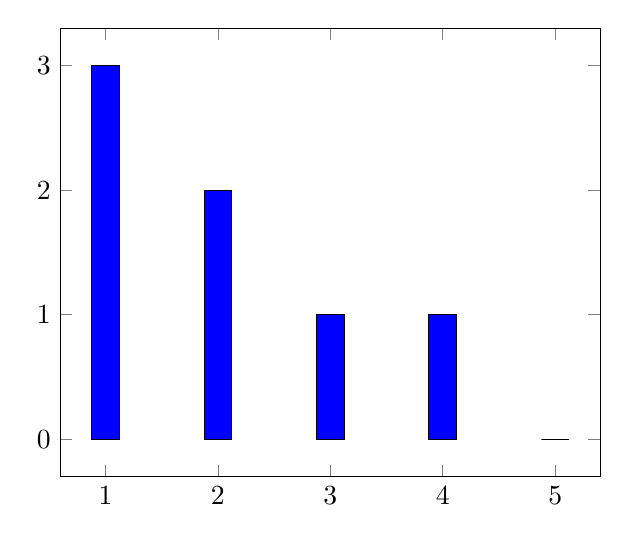
\begin{tikzpicture}
	%\label{bar:results_first}
		\begin{axis}[
			symbolic x coords={1, 2, 3, 4, 5},
			xtick=data
			]
			\addplot[ybar,fill=blue] coordinates {
				(1,  3)
				(2,  2)
				(3,  1)
				(4,  1)
				(5,  0)
			};
		\end{axis}
	\end{tikzpicture}
	\caption{Fråga 1.1: Hur väl stämmer hjälprutan version 1 överens med din prototyp?}
\end{figure}

\begin{figure}[H]
  \centering
  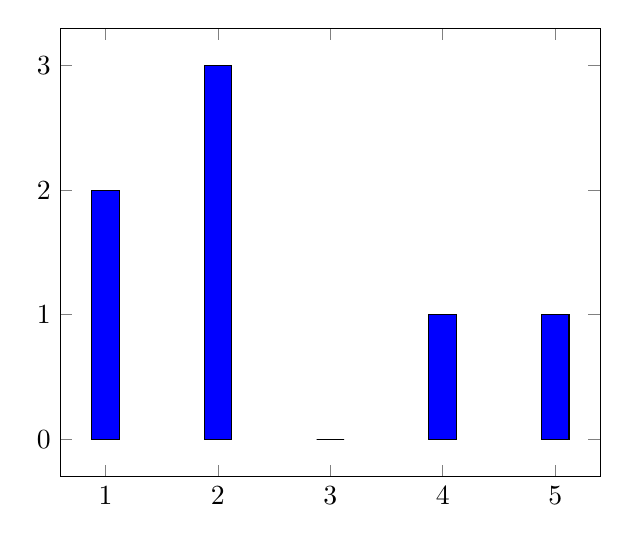
\begin{tikzpicture}
  %\label{bar:results_first}
    \begin{axis}[
      symbolic x coords={1, 2, 3, 4, 5},
      xtick=data
      ]
      \addplot[ybar,fill=blue] coordinates {
        (1,  2)
        (2,  3)
        (3,  0)
        (4,  1)
        (5,  1)
      };
    \end{axis}
  \end{tikzpicture}
  \caption{Fråga 1.2: Hur nöjd är du med resultatet i hjälprutan version 1?}
\end{figure}

\begin{figure}[H]
  \centering
  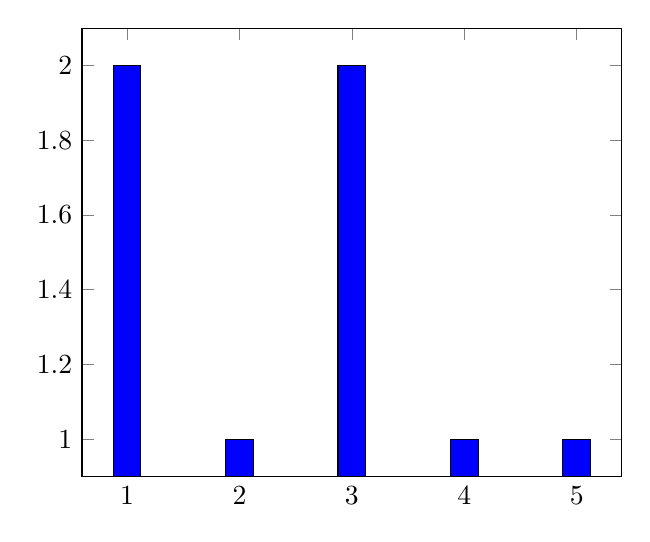
\begin{tikzpicture}
  %\label{bar:results_first}
    \begin{axis}[
      symbolic x coords={1, 2, 3, 4, 5},
      xtick=data
      ]
      \addplot[ybar,fill=blue] coordinates {
        (1,  2)
        (2,  1)
        (3,  2)
        (4,  1)
        (5,  1)
      };
    \end{axis}
  \end{tikzpicture}
  \caption{Fråga 2.1: Hur väl stämmer hjälprutan version 2 överens med din prototyp?}
\end{figure}

\begin{figure}[H]
  \centering
  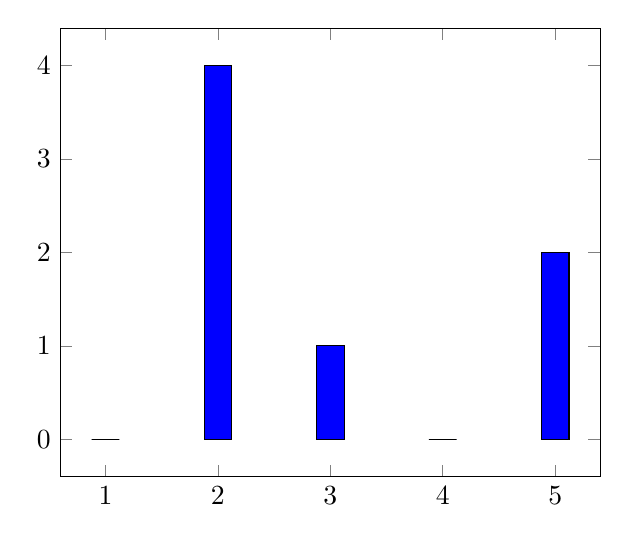
\begin{tikzpicture}
  %\label{bar:results_first}
    \begin{axis}[
      symbolic x coords={1, 2, 3, 4, 5},
      xtick=data
      ]
      \addplot[ybar,fill=blue] coordinates {
        (1,  0)
        (2,  4)
        (3,  1)
        (4,  0)
        (5,  2)
      };
    \end{axis}
  \end{tikzpicture}
  \caption{Fråga 2.2: Hur nöjd är du med resultatet i hjälprutan version 2?}
\end{figure}

\begin{figure}[H]
  \centering
  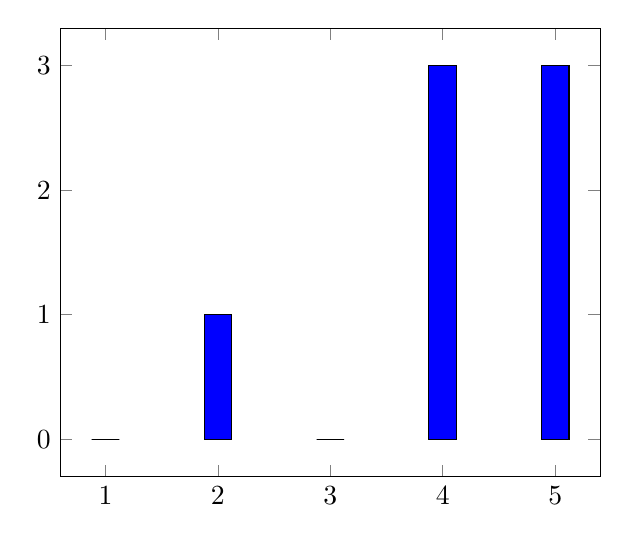
\begin{tikzpicture}
  %\label{bar:results_first}
    \begin{axis}[
      symbolic x coords={1, 2, 3, 4, 5},
      xtick=data
      ]
      \addplot[ybar,fill=blue] coordinates {
        (1,  0)
        (2,  1)
        (3,  0)
        (4,  3)
        (5,  3)
      };
    \end{axis}
  \end{tikzpicture}
  \caption{Fråga 3.1: Hur väl stämmer hjälprutan version 3 överens med din prototyp?}
\end{figure}

\begin{figure}[H]
  \centering
  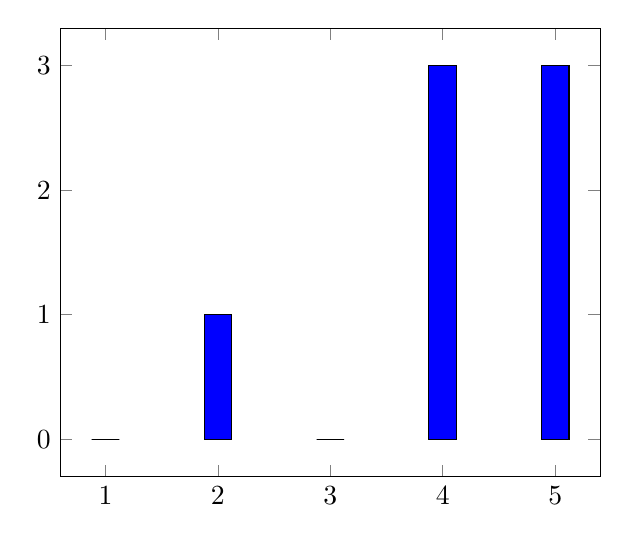
\begin{tikzpicture}
  %\label{bar:results_first}
    \begin{axis}[
      symbolic x coords={1, 2, 3, 4, 5},
      xtick=data
      ]
      \addplot[ybar,fill=blue] coordinates {
        (1,  0)
        (2,  1)
        (3,  0)
        (4,  3)
        (5,  3)
      };
    \end{axis}
  \end{tikzpicture}
  \caption{Fråga 3.2: Hur nöjd är du med resultatet i hjälprutan version 3?}
\end{figure}

\subsection{Tabellen i den detaljerade vyn}
\begin{figure}[H]
  \centering
  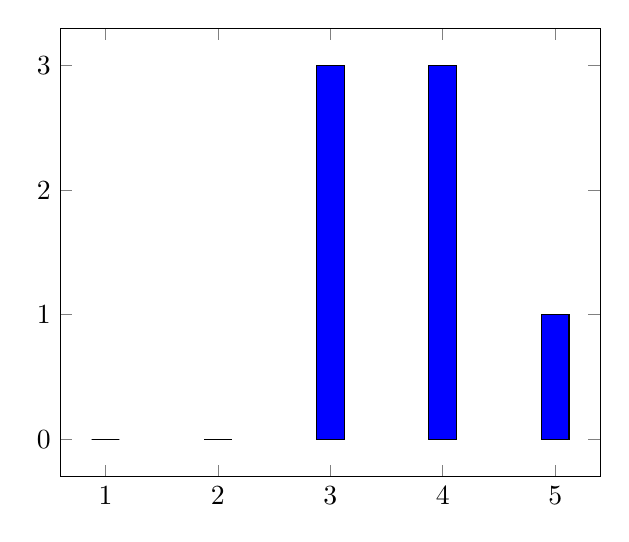
\begin{tikzpicture}
  %\label{bar:results_first}
    \begin{axis}[
      symbolic x coords={1, 2, 3, 4, 5},
      xtick=data
      ]
      \addplot[ybar,fill=blue] coordinates {
        (1,  0)
        (2,  0)
        (3,  3)
        (4,  3)
        (5,  1)
      };
    \end{axis}
  \end{tikzpicture}
  \caption{Fråga 4.1: Hur väl stämmer prototypen överens med din initiala bild av prototypens utseende?}
\end{figure}

\begin{figure}[H]
  \centering
  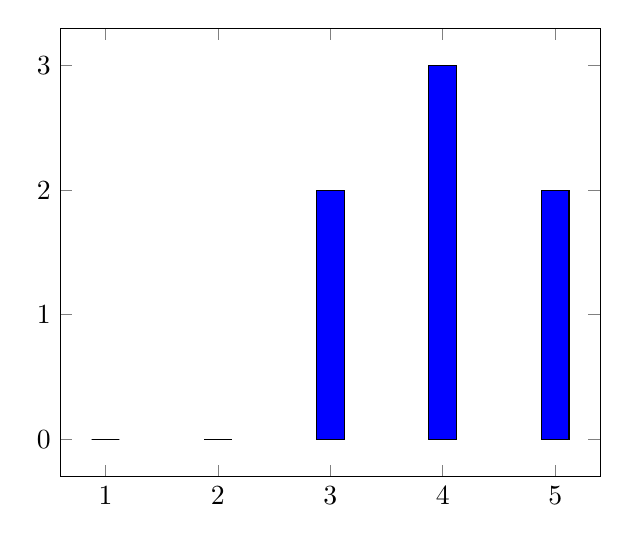
\begin{tikzpicture}
  %\label{bar:results_first}
    \begin{axis}[
      symbolic x coords={1, 2, 3, 4, 5},
      xtick=data
      ]
      \addplot[ybar,fill=blue] coordinates {
        (1,  0)
        (2,  0)
        (3,  2)
        (4,  3)
        (5,  2)
      };
    \end{axis}
  \end{tikzpicture}
  \caption{Fråga 4.2: Hur nöjd är du med tabellens utseende i denna prototyp?}
\end{figure}

\begin{figure}[H]
  \centering
  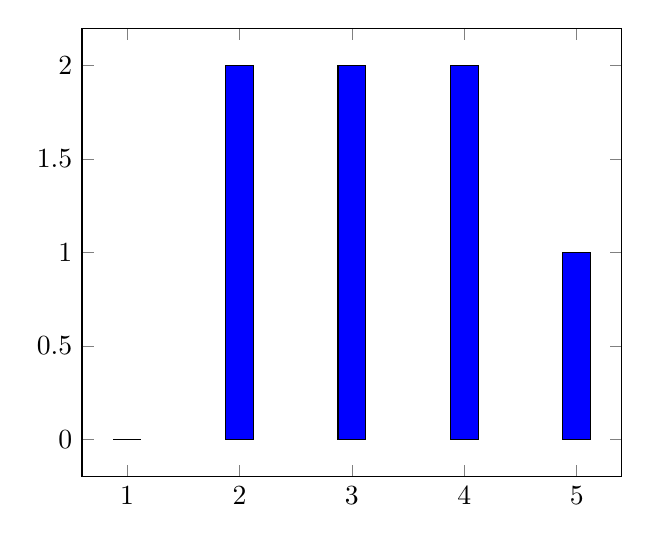
\begin{tikzpicture}
  %\label{bar:results_first}
    \begin{axis}[
      symbolic x coords={1, 2, 3, 4, 5},
      xtick=data
      ]
      \addplot[ybar,fill=blue] coordinates {
        (1,  0)
        (2,  2)
        (3,  2)
        (4,  2)
        (5,  1)
      };
    \end{axis}
  \end{tikzpicture}
  \caption{Fråga 5.1: Hur väl stämmer tabellen version 1 överens med gruppens prototyp?}
\end{figure}

\begin{figure}[H]
  \centering
  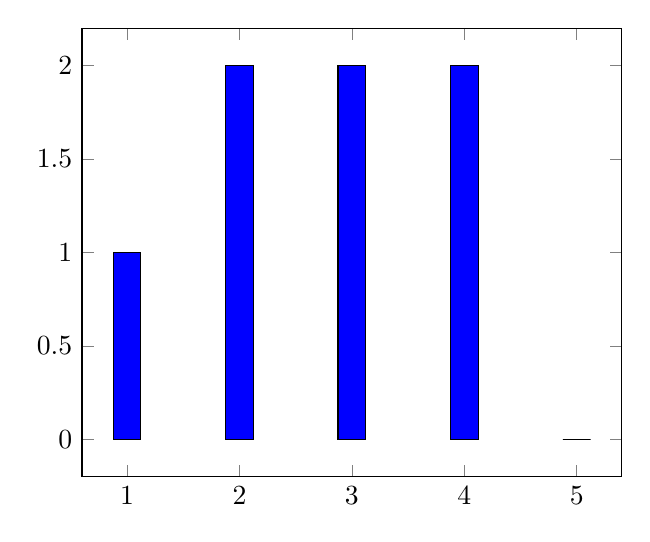
\begin{tikzpicture}
  %\label{bar:results_first}
    \begin{axis}[
      symbolic x coords={1, 2, 3, 4, 5},
      xtick=data
      ]
      \addplot[ybar,fill=blue] coordinates {
        (1,  1)
        (2,  2)
        (3,  2)
        (4,  2)
        (5,  0)
      };
    \end{axis}
  \end{tikzpicture}
  \caption{Fråga 5.2: Hur nöjd är du med resultatet i tabellen version 1?}
\end{figure}

\begin{figure}[H]
  \centering
  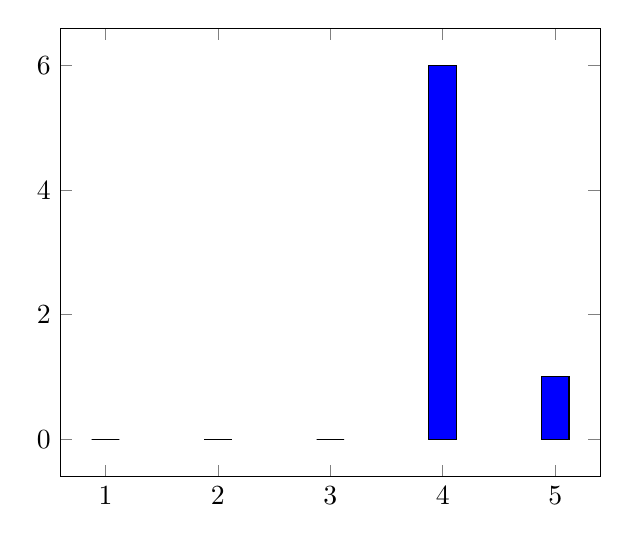
\begin{tikzpicture}
  %\label{bar:results_first}
    \begin{axis}[
      symbolic x coords={1, 2, 3, 4, 5},
      xtick=data
      ]
      \addplot[ybar,fill=blue] coordinates {
        (1,  0)
        (2,  0)
        (3,  0)
        (4,  6)
        (5,  1)
      };
    \end{axis}
  \end{tikzpicture}
  \caption{Fråga 6.1: Hur väl stämmer tabellen version 2 överens med gruppens prototyp?}
\end{figure}

\begin{figure}[H]
  \centering
  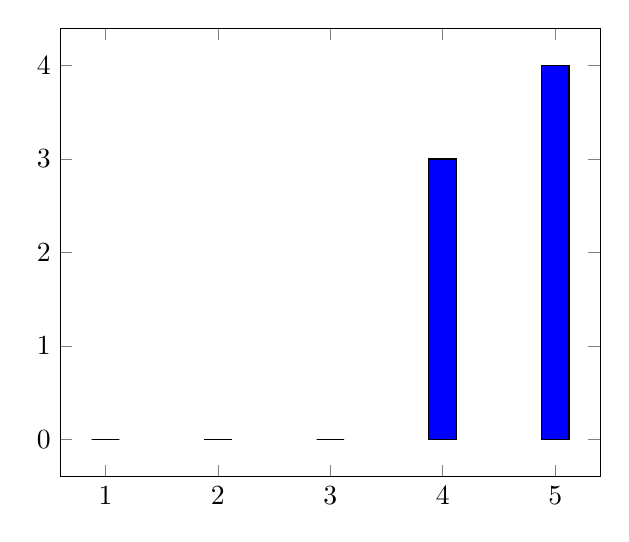
\begin{tikzpicture}
  %\label{bar:results_first}
    \begin{axis}[
      symbolic x coords={1, 2, 3, 4, 5},
      xtick=data
      ]
      \addplot[ybar,fill=blue] coordinates {
        (1,  0)
        (2,  0)
        (3,  0)
        (4,  3)
        (5,  4)
      };
    \end{axis}
  \end{tikzpicture}
  \caption{Fråga 6.2: Hur nöjd är du med resultatet i tabellen version 2?}
\end{figure}

\subsection{Avslutande frågor}
\begin{figure}[H]
  \centering
  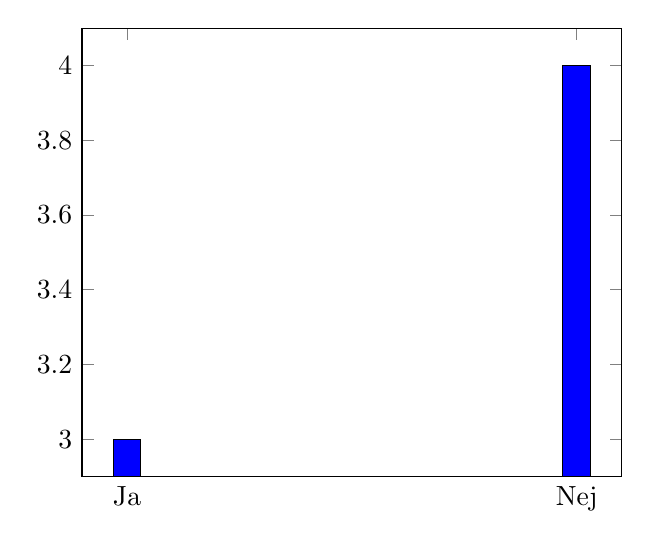
\begin{tikzpicture}
  %\label{bar:results_first}
    \begin{axis}[
      symbolic x coords={Ja, Nej},
      xtick=data
      ]
      \addplot[ybar,fill=blue] coordinates {
        (Ja,   3)
        (Nej,  4)
      };
    \end{axis}
  \end{tikzpicture}
  \caption{Fråga 7.1: Upplever du att du har fått göra om features för att resultatets utseende inte stämde överens med andra gruppmedlemmars bild av det?}
\end{figure}

\begin{figure}[H]
  \centering
  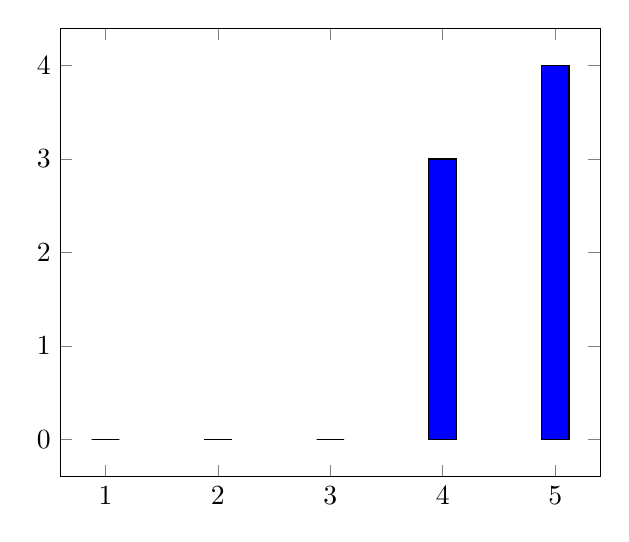
\begin{tikzpicture}
  %\label{bar:results_first}
    \begin{axis}[
      symbolic x coords={1, 2, 3, 4, 5},
      xtick=data
      ]
      \addplot[ybar,fill=blue] coordinates {
        (1,  0)
        (2,  0)
        (3,  0)
        (4,  3)
        (5,  4)
      };
    \end{axis}
  \end{tikzpicture}
  \caption{Fråga 7.2: Tycker du att det har underlättat utvecklingen att jobba med prototyper?}
\end{figure}

\begin{table}[h!]
  \caption{Fråga 7.3: På vilket/vilka sätt har det underlättat/inte underlättat?}
  \def\arraystretch{1.5}
  \begin{adjustbox}{max width=\textwidth}
    \begin{tabularx}{\textwidth}{ | X |}
      \hline
      \textbf{Svar} \\
      \hline
      Man får mindre iterationer om man följer en specad standard då personer får vara nöjda när den är uppnådd. \\
      \hline
      Det ger en målbild att jobba mot och något som kan användas som diskussionsunderlag för hur resten av prototypandet ska fortsätta \\
      \hline
      Man får en tydlig bild av hur slutresultat förväntas se ut. \\
      \hline 
      Som en tydlig kravspec att följa \\
      \hline 
      Många designbeslut finns tydligt visualiserade och det behövdes för att man skulle veta hur feature'n skulle anpassas. \\
      \hline 
      Lättare att ha gemensam bild av vad som ska göras. \\
      \hline 
      En bra startbild \\
      \hline  
    \end{tabularx}
  \end{adjustbox}
  \label{tab:prototyp_enkat_ease}
\end{table}

\begin{figure}[H]
  \centering
  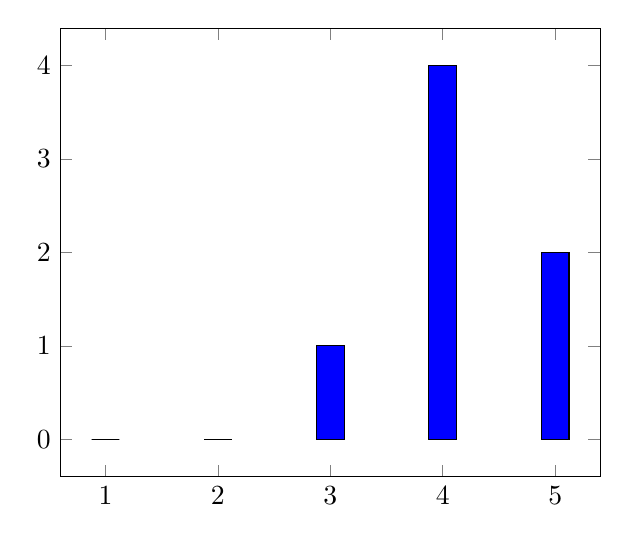
\begin{tikzpicture}
  %\label{bar:results_first}
    \begin{axis}[
      symbolic x coords={1, 2, 3, 4, 5},
      xtick=data
      ]
      \addplot[ybar,fill=blue] coordinates {
        (1,  0)
        (2,  0)
        (3,  1)
        (4,  4)
        (5,  2)
      };
    \end{axis}
  \end{tikzpicture}
  \caption{Fråga 7.4: Tycker du att tiden som spenderats på att ta fram prototyper har varit väl spenderad tid?}
\end{figure}

\begin{figure}[H]
  \centering
  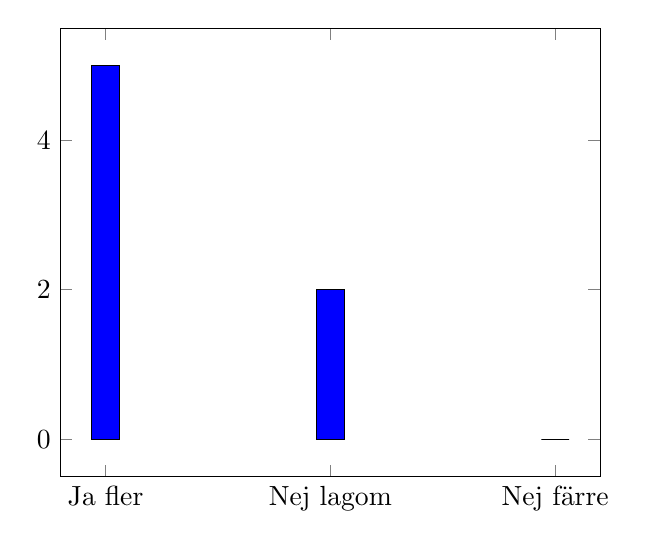
\begin{tikzpicture}
  %\label{bar:results_first}
    \begin{axis}[
      symbolic x coords={Ja fler, Nej lagom, Nej färre},
      xtick=data
      ]
      \addplot[ybar,fill=blue] coordinates {
        (Ja fler,    5)
        (Nej lagom,  2)
        (Nej färre,  0)
      };
    \end{axis}
  \end{tikzpicture}
  \caption{Fråga 7.5: Hade du velat att gruppen hade tagit fram prototyper för fler features?}
\end{figure}

\begin{figure}[H]
  \centering
  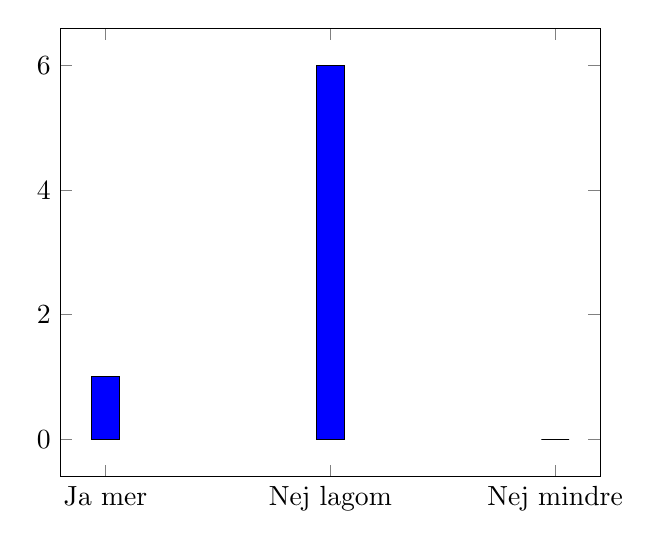
\begin{tikzpicture}
  %\label{bar:results_first}
    \begin{axis}[
      symbolic x coords={Ja mer, Nej lagom, Nej mindre},
      xtick=data
      ]
      \addplot[ybar,fill=blue] coordinates {
        (Ja mer,     1)
        (Nej lagom,  6)
        (Nej mindre, 0)
      };
    \end{axis}
  \end{tikzpicture}
  \caption{Fråga 7.6: Hade du velat att gruppen hade utvecklat de existerande prototyperna mer?}
\end{figure}

\begin{table}[h!]
  \caption{Fråga 7.7: Kommentarer (frivillig)}
  \def\arraystretch{1.5}
  \begin{adjustbox}{max width=\textwidth}
    \begin{tabularx}{\textwidth}{ | X |}
      \hline
      \textbf{Svar} \\
      \hline
      Prototyper är ett bra verktyg så att gruppen kan få en enhetlig bild av vad målet ska bli \\
      \hline
      Skönt att andra säger hur de vill ha det så man får flera perspektiv \\
      \hline  
    \end{tabularx}
  \end{adjustbox}
  \label{tab:prototyp_enkat_comments
}
\end{table}
\chapter{\hspace{2.6em} Frågeformulär för utvärdering av hur verktyg har använts för utveckling av mjukvara}
\label{cha:verktyg_enkat_fragor}

\begin{table}[h!]
  \centering
  \caption{En tabell över frågorna i frågeformuläret om hur verktyg har använts för utveckling av mjukvara.}
  \def\arraystretch{1.5}
  \begin{adjustbox}{max width=\textwidth}
    \begin{tabularx}{\textwidth}{ | l | X | l |}
      \hline
      \textbf{Nummer} & \textbf{Fråga} & \textbf{Svarstyp} \\
      \hline
      1 & Hur mycket av din projekttid har du lagt på att utveckla mjukvara? (utöver obligatoriska möten och seminarium och så) & Skala 1-10 \\
      \hline
      2 & Vilken editor har du främst använt för att koda i appen? & Alternativ \\
      \hline 
      3 & Varför valde du denna editor? & Alternativ \\
      \hline
      4 & Hur tycker du att ditt val av editor har påverkat utvecklingen av mjukvara? & Skala 1-5 \\
      \hline
      5 & Hur tycker du att Git har påverkat utvecklingen av mjukvara? & Skala 1-5 \\
      \hline
      6 & Har du fått hjälp med Git när du behövt? & Skala 1-5 \\
      \hline
      7 & Hur tycker du att Trello har påverkat utvecklingen av mjukvara? & Skala 1-5 \\
      \hline
      8 & Hur tycker du att Slack har påverkat utvecklingen av mjukvara? & Skala 1-5 \\
      \hline
      9 & Vilka problem ser du med de verktyg vi använt för att utveckla mjukvara? & Text \\
      \hline
      10 & Vilka problem ser du med hur verktygen har använts av gruppmedlemmarna? & Text \\
      \hline
      11 & Om du skulle vilja ändra något med verktygen eller hur de används, vad skulle det vara? & Text \\
      \hline
      12 & Om du kan, hitta på ett verktyg som vi skulle kunna använda för att ytterligare underlätta för utvecklingen av mjukvara i vår grupp. & Text \\
      \hline
    \end{tabularx}
  \end{adjustbox}
\end{table}

\pagebreak

\chapter{\hspace{2.6em} Resultat från utvärdering av hur verktyg har använts för utveckling av mjukvara}
\label{cha:verktyg_enkat_resultat}

\begin{figure}[!h]
	\centering
	\caption{Fråga 1: Hur mycket av din projekttid har du lagt på att utveckla mjukvara? (utöver obligatoriska möten och seminarium och så). Från ``Har ej rört någon kod`` till ``Har spenderat all min tid bara programmera``.}
	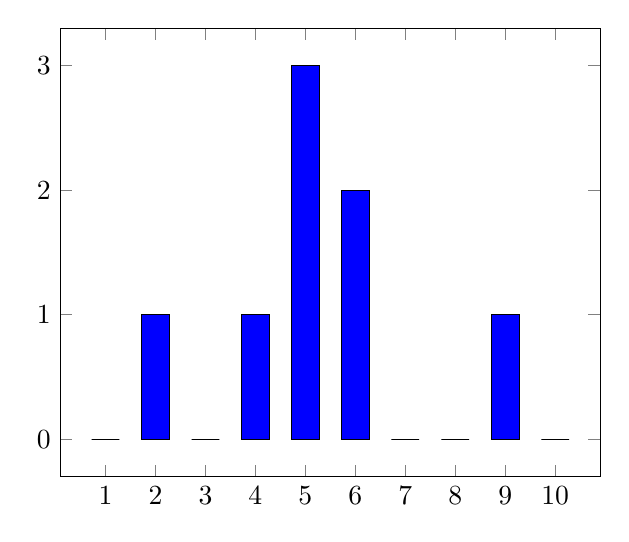
\begin{tikzpicture}
	%\label{bar:results_first}
		\begin{axis}[
			symbolic x coords={1, 2, 3, 4, 5, 6, 7, 8, 9, 10},
			xtick=data
			]
			\addplot[ybar,fill=blue] coordinates {
				(1,  0)
				(2,  1)
				(3,  0)
				(4,  1)
				(5,  3)
				(6,  2)
				(7,  0)
				(8,  0)
				(9,  1)
				(10,  0)
			};
		\end{axis}
	\end{tikzpicture}
\end{figure}

\begin{figure}[!h]
	\centering
	\caption{Fråga 2: Vilken editor har du främst använt för att koda i appen?}
	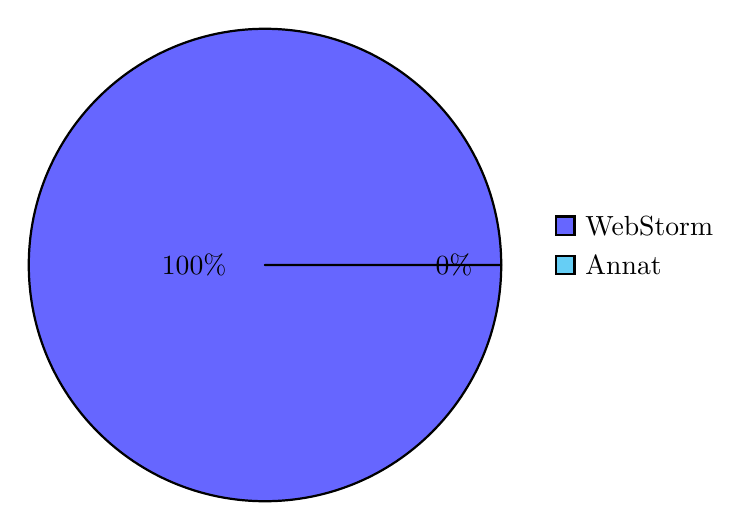
\begin{tikzpicture}
\pie [text=legend]{100/WebStorm, 0/Annat}
\end{tikzpicture}
\end{figure}

\begin{figure}[!h]
	\centering
	\caption{Fråga 3: Varför valde du denna editor?}
	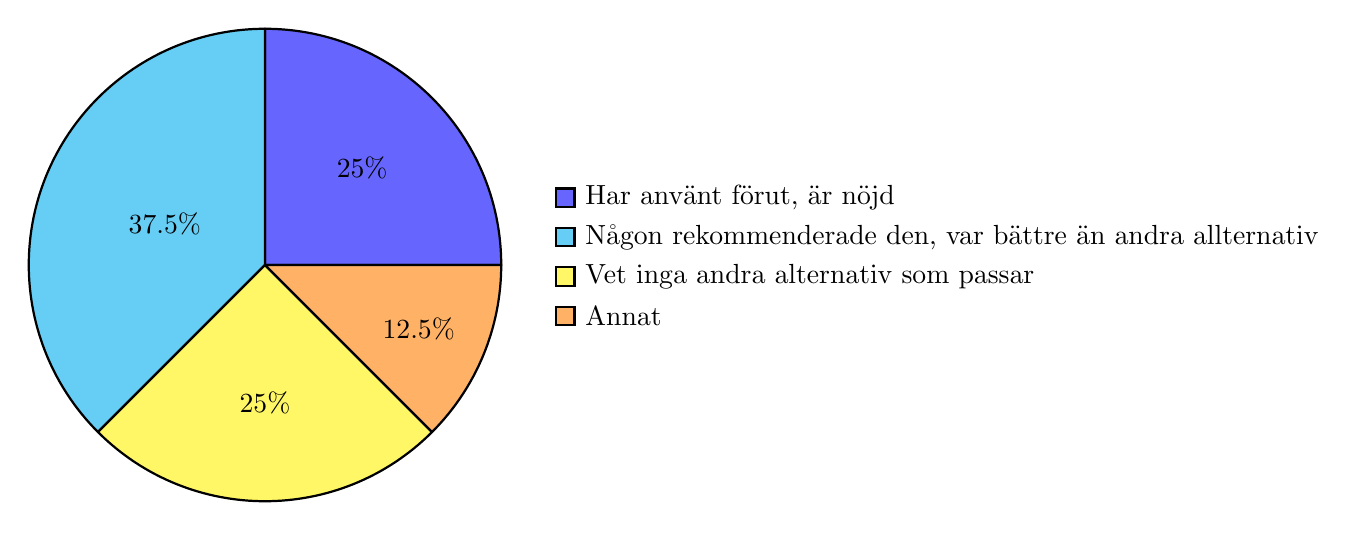
\begin{tikzpicture}
\pie [text=legend]{25/{Har använt förut, är nöjd}, 37.5/{Någon rekommenderade den, var
bättre än andra allternativ}, 25/{Vet inga andra alternativ som passar}, 12.5/{Annat}}
\end{tikzpicture}
\end{figure}

\begin{figure}[!h]
	\centering
	\caption{Fråga 4: Hur tycker du att ditt val av editor har påverkat utvecklingen av mjukvara? Från ``Försämrat utvecklingen`` till ``Underlättat utvecklingen väldigt mycket``.}
	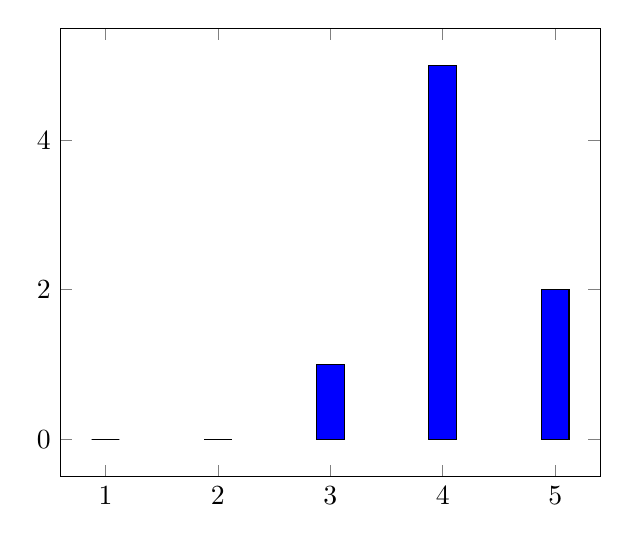
\begin{tikzpicture}
	%\label{bar:results_first}
		\begin{axis}[
			symbolic x coords={1, 2, 3, 4, 5},
			xtick=data
			]
			\addplot[ybar,fill=blue] coordinates {
				(1,  0)
				(2,  0)
				(3,  1)
				(4,  5)
				(5,  2)
			};
		\end{axis}
	\end{tikzpicture}
\end{figure}

\begin{figure}[!h]
	\centering
	\caption{Fråga 5: Hur tycker du att Git har påverkat utvecklingen av mjukvara? Från ``Försämrat utvecklingen`` till ``Underlättat utvecklingen väldigt mycket``.}
	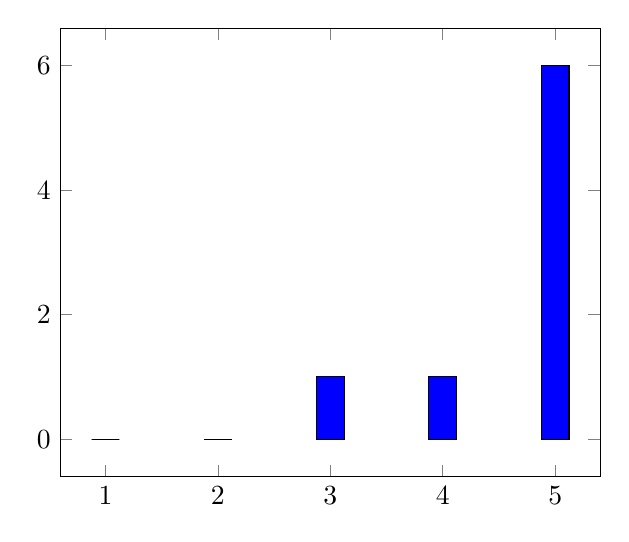
\begin{tikzpicture}
	%\label{bar:results_first}
		\begin{axis}[
			symbolic x coords={1, 2, 3, 4, 5},
			xtick=data
			]
			\addplot[ybar,fill=blue] coordinates {
				(1,  0)
				(2,  0)
				(3,  1)
				(4,  1)
				(5,  6)
			};
		\end{axis}
	\end{tikzpicture}
\end{figure}

\begin{figure}[!h]
	\centering
	\caption{Fråga 6: Har du fått hjälp med Git när du behövt? Från ``Nej`` till ``Alltid``.}
	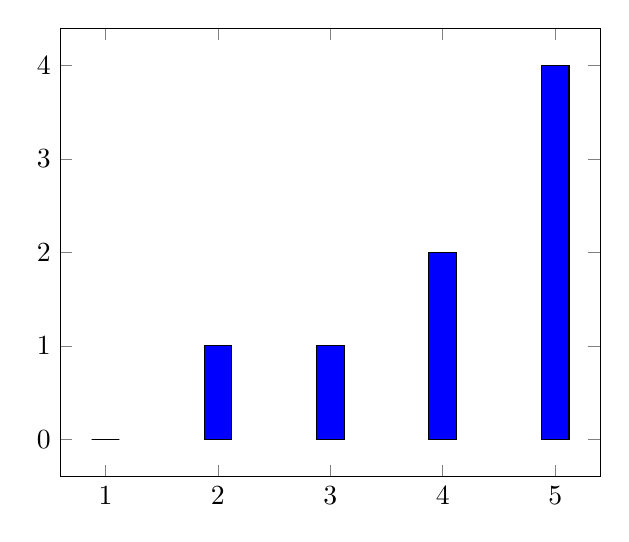
\begin{tikzpicture}
	%\label{bar:results_first}
		\begin{axis}[
			symbolic x coords={1, 2, 3, 4, 5},
			xtick=data
			]
			\addplot[ybar,fill=blue] coordinates {
				(1,  0)
				(2,  1)
				(3,  1)
				(4,  2)
				(5,  4)
			};
		\end{axis}
	\end{tikzpicture}
\end{figure}

\begin{figure}[!h]
	\centering
	\caption{Fråga 7: Hur tycker du att Trello har påverkat utvecklingen av mjukvara? Från ``Försämrat utvecklingen`` till ``Underlättat utvecklingen väldigt mycket``.}
	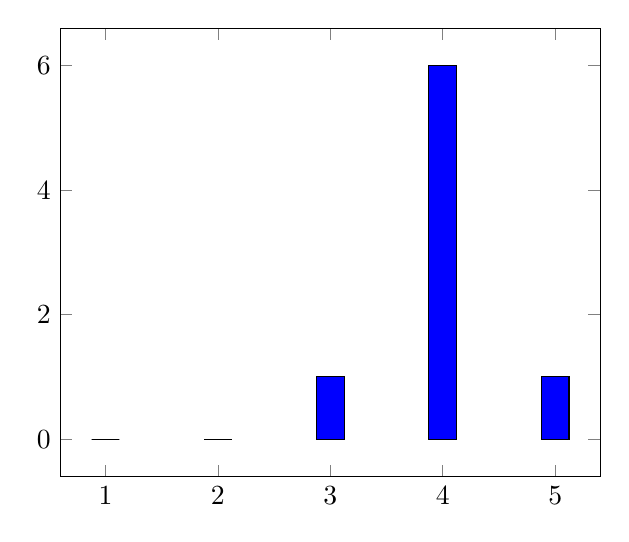
\begin{tikzpicture}
	%\label{bar:results_first}
		\begin{axis}[
			symbolic x coords={1, 2, 3, 4, 5},
			xtick=data
			]
			\addplot[ybar,fill=blue] coordinates {
				(1,  0)
				(2,  0)
				(3,  1)
				(4,  6)
				(5,  1)
			};
		\end{axis}
	\end{tikzpicture}
\end{figure}

\begin{figure}[!h]
	\centering
	\caption{Fråga 8: Hur tycker du att Slack har påverkat utvecklingen av mjukvara? Från ``Försämrat utvecklingen`` till ``Underlättat utvecklingen väldigt mycket``.}
	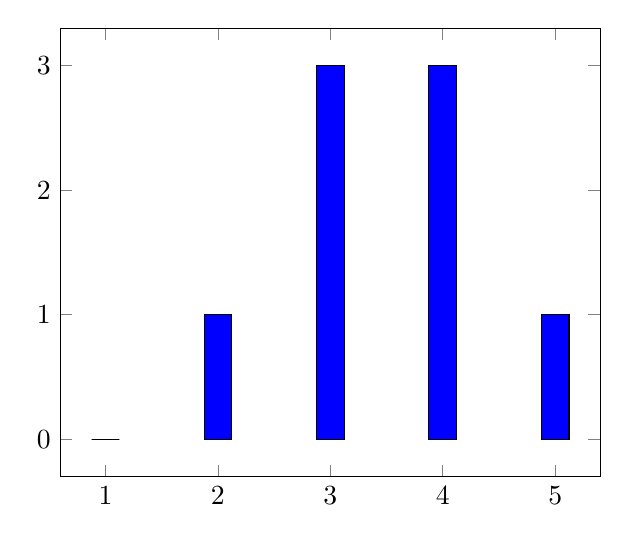
\begin{tikzpicture}
	%\label{bar:results_first}
		\begin{axis}[
			symbolic x coords={1, 2, 3, 4, 5},
			xtick=data
			]
			\addplot[ybar,fill=blue] coordinates {
				(1,  0)
				(2,  1)
				(3,  3)
				(4,  3)
				(5,  1)
			};
		\end{axis}
	\end{tikzpicture}
\end{figure}

\begin{table}[h!]
\centering
  \caption{Fråga 9: Vilka problem ser du med de verktyg vi använt för att utveckla mjukvara?}
  \def\arraystretch{1.5}
  \begin{adjustbox}{max width=\textwidth}
    \begin{tabularx}{\textwidth}{| X |}
      \hline
      \textbf{Svar} \\
      \hline
      Ibland saknas det kompetens för att utnyttja verktyget till fullo \\
      \hline
      Inga direkta problem. \\
      \hline
      Har svårt att se problem då jag inte har bra koll på många andra alternativ. Förutom det så har jag inte upplevt några problem.\\
      \hline 
      Ser inga problem med dem\\
      \hline 
      Dålig disciplin/konventioner i Slack och Trello leder till oordning \\
      \hline 
      Git: Viss inlärningströskel. Webstorm: aningen resurskrävande på laptop. Slack: Mycket meddelanden, som man inte alltid läser och därför kanske missar något viktigt. Trello: Inga problem.\\
      \hline 
      Verkar vara en stabil editor\\
      \hline  
      Inga, är bekväm med allt.\\
      \hline
    \end{tabularx}
  \end{adjustbox}
\end{table}

\begin{table}[h!]
\centering
  \caption{Fråga 10: Vilka problem ser du med hur verktygen har använts av gruppmedlemmarna?}
  \def\arraystretch{1.5}
  \begin{adjustbox}{max width=\textwidth}
    \begin{tabularx}{\textwidth}{| X |}
      \hline
      \textbf{Svar} \\
      \hline
      Man har använd verktygen olika och detta kan ha lätt till förvirring, tillexempel kommentarer på trellokort \\
      \hline
      Alla har inte varit på samma nivå med tex Git och vissa har inte brytt sig om att följa de regler vi satt upp. \\
      \hline
      Varierande kunskap har definitivt påverkat hur folk använder verktygen, det kan ibland ha satt käppar i hjulen men inget allvarligt så det är svårt att specificera.\\
      \hline 
      Vissa har inte lärt sig git tillräckligt bra\\
      \hline 
      Gruppmedlemmar skulle behöva mer kompetens inom verktygen så att ingen skriver t.ex. "git rm .". \\
      \hline 
      Inget egentligen\\
      \hline 
      Inget man reflekterat över, man bara kör på\\
      \hline  
      Git add . Skulle kunna ha haft nån kort genomgång hur man gör.\\
      \hline
    \end{tabularx}
  \end{adjustbox}
\end{table}

\begin{table}[h!]
\centering
  \caption{Fråga 11: Om du skulle vilja ändra något med verktygen eller hur de används, vad skulle det vara?}
  \def\arraystretch{1.5}
  \begin{adjustbox}{max width=\textwidth}
    \begin{tabularx}{\textwidth}{| X |}
      \hline
      \textbf{Svar} \\
      \hline
      Inbyggda videokonferenser i Slack. Prioriteringsbara kort i Trello. \\
      \hline
      Att hålla mer fokuserade diskussioner i Trello-kort istället för en Slack-chatt hade gjort problem i utvecklingen lättare att följa. \\
      \hline
      Ingenting\\
      \hline 
      Svårt att veta när man inte har jobbat i en annan editor för webbprogrammering tidigare så man kan inte jämnföra.\\
      \hline 
    \end{tabularx}
  \end{adjustbox}
\end{table}

\begin{table}[h!]
\centering
  \caption{Fråga 12: Om du kan, hitta på ett verktyg som vi skulle kunna använda för att ytterligare underlätta för utvecklingen av mjukvara i vår grupp.}
  \def\arraystretch{1.5}
  \begin{adjustbox}{max width=\textwidth}
    \begin{tabularx}{\textwidth}{| X |}
      \hline
      \textbf{Svar} \\
      \hline
      Ett övergripande planeringsverktyg för att tydligt se flödesschema på vilka uppgifter som bygger på varandra och i vilken ordning saker behöver göras. Trello saknar den biten. \\
      \hline
      Ett system där en process som kräver validering och testning innan kod kan pushas hade varit användbart för att säkerställa kvalitet. Gärna integrerat (eller med tillhörande) Trello-funktionalitet för att spåra arbetet \\
      \hline
      en voice-to-text så man slipper använda händerna.\\
      \hline 
    \end{tabularx}
  \end{adjustbox}
\end{table}
\chapter{\hspace{2.6em} Frågeformulär för utvärdering av sprint}
\label{cha:team_utvardering}
På nästa sida visas utvärderingsformuläret som användes under retrospektiven.
\includepdf[scale=0.9]{Teamutvardering2017}

\chapter{\hspace{2.6em} Formulär för utvärdering av retrospektiv}
\label{cha:retrospektiv_eval_form}

\begin{figure}[h]
  \centering
  \includegraphics[scale=0.7]{retro_eval_form_1}
  \caption{Formulär för utvärdering av retrospektiv del 1}
\end{figure}

\begin{figure}[h]
  \centering
  \includegraphics[scale=0.7]{retro_eval_form_2}
  \caption{Formulär för utvärdering av retrospektiv del 2}
\end{figure}

\chapter{\hspace{2.6em} Sammanställning av data från retrospektiv}
\label{cha:sammanstallning_av_data}
På nästa sida redovisas en sammanställning av data från retrospektiven i tabellform.
\includepdf{retro_data_sammanstallning}

\section{Bra och Bättre}
\label{sec:bra_och_battre}
\begin{figure}[h]
  \centering
  \includegraphics[scale=0.65]{retro_data_bra_och_battre}
\end{figure}

\clearpage
\printbibliography

\end{document}


